\documentclass{report}

\usepackage[screen,nopanel,sectionbreak]{pdfscreen}
\margins{0.5 cm}{0.5 cm}{0.5 cm}{1.0 cm}
%\screensize{15 cm}{20 cm} % Raz'on 3:4
%\screensize{12 cm}{16 cm}
\screensize{9 cm}{16 cm}
\overlayempty
%\overlay{overlay}
%\definecolor{mybg}{rgb}{1,0.9,0.7}
\definecolor{mybg}{rgb}{1.0,1.0,1.0}
\backgroundcolor{mybg}

\let\st\relax % Avoid -> LaTeX Error: Command \st already defined.
\usepackage{pdfcomment}
\usepackage{xcolor}
\newcommand{\popup}[2]{\pdftooltip{\textcolor{blue}{#1}}{#2}}

\usepackage{lastpage}
\usepackage{fancyhdr}
\renewcommand{\headrulewidth}{0pt}
\pagestyle{fancy} % for fancydr package
%\fancyhf{}
\pagenumbering{arabic} % Reseteamos las p'aginas
% Cabeceras no todo en may'usculas
%\renewcommand{\sectionmark}[1]{\markright{\thesection\ #1}}
% Definici'on de las cabeceras
\lhead{} \rhead{} \chead{}
%\lfoot[\fancyplain{}{\sf\thepage}]{\color{blue}\fancyplain{}{\sf\rightmark}}
%\lfoot[]{}
%\rfoot[\fancyplain{}{\sf\leftmark}]{\color{red}\fancyplain{}{\sf\thepage}}
%\rfoot[]{}
\cfoot[]{}
\rfoot{\colorbox{mybg}{\footnotesize\color{red}\thepage/\pageref{LastPage}}}
\setlength{\footskip}{12.0pt}

\usepackage{graphicx}
\graphicspath{{imgs}{figs}{notebooks}{.}{gnuplot}{modules}}

\usepackage{caption}
\captionsetup[figure]{skip=1pt}
\captionsetup[table]{skip=1pt}
\setlength{\textfloatsep}{0pt}
\setlength{\floatsep}{0pt}
\setlength{\intextsep}{0pt}
\setlength{\abovecaptionskip}{0pt}
\setlength{\belowcaptionskip}{0pt}

\usepackage[acronym]{glossaries}
\makeglossaries
\newacronym{TFT}{TFT}{{Thin-Film Transistor}}
\newacronym{GI}{GI}{{GastroIntestinal}}
\newacronym{SNR}{SNR}{{Signal-to-Noise Ratio}}
\newacronym{PNI}{PNI}{{Planar Nuclear Imaging}}
\newacronym{CT}{CT}{{Computed Tomography}}
\newacronym{LAC}{LAC}{{Linear Attenuacion Coefficient}}
\newacronym{PET}{PET}{{Positron Emission Tomography}}
\newacronym{SPECT}{SPECT}{{Single Photon Emission Computed Tomography}}
\newacronym{MRI}{MRI}{{Magnetic Resonance Imaging}}
\newacronym{RF}{RF}{{Radio Frequency}}
\newacronym{EM}{EM}{{Electro Magnetic}}
%\newacronym{CSF}{CSF}{CerebroSpinal Fluid}
\newacronym{PD}{PD}{{Proton Density}}
\newacronym{FOV}{FOV}{{Field Of View}}

\newacronym{KB}{KB}{{KiloByte}}
\newacronym{MB}{MB}{{MegaByte}}
\newacronym{GB}{GB}{{GigaByte}}
\newacronym{TB}{TB}{TeraByte}
\newacronym{PB}{PB}{PetaByte}

\newacronym{RAM}{RAM}{{Random Access Memory}}
\newacronym{ROM}{ROM}{{Read Only Memory}}
\newacronym{WORM}{WORM}{{Write Once, Read Many}}
\newacronym{CD}{CD}{{Compact Disk}}
\newacronym{DVD}{DVD}{{Digital Versatile Disk}}
\newacronym{CD-ROM}{CD-ROM}{{Compact Disc - Read-Only Memory}}
\newacronym{DVD-ROM}{DVD-ROM}{Digital Versatile Disk - Read-Only Memory (see \gls{DVD})}
\newacronym{CD-R}{CD-R}{{Compact Disc - Recordable}}
\newacronym{CD-RW}{CD-RW}{{Compact Disc - ReWritable}}
\newacronym{RAID}{RAID}{{Redundant Array of Independent Disks}}
\newacronym{LAN}{LAN}{{Local Area Network}}
\newacronym{NAS}{{NAS}}{Network-Attached Storage}
\newacronym{HDD}{HDD}{{Hard Disk Drive}}
\newacronym{SSD}{SSD}{{Solid State Drive}}
\newacronym{PACS}{PACS}{{Picture Archiving and Communication System}}

\newacronym{PNG}{PNG}{{Portable Network Graphics}}
\newacronym{W3C}{W3C}{{World Wide Web Consortium}}
\newacronym{RGBA}{RGBA}{{Red, Green, Blue, Alpha}}
\newacronym{APNG}{APNG}{{Animated PNG}}

\newacronym{JPEG}{JPEG}{{Joint Photographic Expert Group}}
\newacronym{ITU}{ITU}{{International Telecommunication Union}}
\newacronym{RGB}{RGB}{{Red, Green, Blue}}
\newacronym{YCbCr}{YCbCr}{{Y-luminance, blue-Crominance, red-Crominance}}
\newacronym{DCT}{DCT}{{Discrete Cosine Transform}}

\newacronym{ISO}{ISO}{{International Organization for Standardization}}
\newacronym{IEC}{IEC}{{International Electrotechnical Commission}}
\newacronym{CIE}{CIE}{{Commission Internationale de l´Éclairage}}
\newacronym{CIELAB}{CIELAB}{{CIE L*a*b*: L*-luminance, a*-chrominance, b*-crominance}}
\newacronym{sRGB}{sRGB}{{standard Red, Green, Blue}xs}
\newacronym{DWT}{DWT}{{Discrete Wavelet Transform}}
\newacronym{ROI}{ROI}{{Region Of Interest}}
\newacronym{EBCOT}{EBCOT}{{Embedded Block Coding with Optimal Truncation}}
\newacronym{JPIP}{JPIP}{{JPeg2000 Interactive Protocol}}
\newacronym{SPIHT}{SPIHT}{{Set Partitioning In Hierarchical Trees}}

\newacronym{MPEG}{MPEG}{{Moving Picture Experts Group}}
\newacronym{DVB}{DVB}{{Digital Video Broadcasting}}
\newacronym{VCD}{VCD}{{Video CD}}
\newacronym{RDO}{RDO}{{Rate/Distortion Optimization}}

\newacronym{VCEG}{VCEG}{{Video Coding Experts Group}}
\newacronym{LPC}{LPC}{{Linear Predictive Coding}}
\newacronym{CABAC}{CABAC}{{Context-Adaptive Binary Arithmetic Coding}}

\newacronym{BER}{BER}{{Bit Error Rate}} 
\newacronym{HTTP}{HTTP}{{Hypertext Transfer Protocol}}
\newacronym{HTTPS}{HTTPS}{{Hypertext Transfer Protocol Secure}}
\newacronym{WWW}{WWW}{{World Wide Web}} 
\newacronym{TCP}{TCP}{{Transmission Control Protocol}}
\newacronym{UDP}{UDP}{{User Datagram Protocol}}
\newacronym{IP}{IP}{{Internet Protocol}}
\newacronym{NAT}{NAT}{{Network Address Translation}}
\newacronym{SSL}{SSL}{{Secure Sockets Layer}}
\newacronym{TLS}{TLS}{{Transport Layer Security}}

\newacronym{CERN}{CERN}{{Conseil Européen pour la Recherche Nucléaire}}
\newacronym{URL}{URL}{Uniform Resource Locator}
\newacronym{HTML}{HTML}{{Hypertext Markup Language}}
\newacronym{GIF}{GIF}{{Graphics Interchange Format}}
\newacronym{PDF}{PDF}{{Portable Document Format}}
\newacronym{SVG}{SVG}{{Scalable Vector Graphics}}
\newacronym{WebP}{WebP}{{Web Picture}}
\newacronym{CSS}{CSS}{{Cascading Style Sheets}}
\newacronym{AAC}{AAC}{{Advanced Audio Coding}}
\newacronym{MP3}{MP3}{{MPEG-1 Audio Layer-3}}
\newacronym{MP4}{MP4}{MPEG-4 (video container)}
\newacronym{AVC}{AVC}{{Advanced Video Coding}}
\newacronym{HEVC}{HEVC}{{High Efficiency Video Coding}}
\newacronym{CTU}{CTU}{{Coding Tree Unit}}
\newacronym{VVC}{VVC}{{Versatile Video Coding}}
\newacronym{VC-1}{VC-1}{{Video Codec 1}}
\newacronym{AV1}{AV1}{{AOMedia Video 1}}
\newacronym{VP9}{VP9}{{VP9}}

\newacronym{DICOM}{DICOM}{{Digital Imaging and Communications in Medicine}}
\newacronym{NEMA}{NEMA}{{National Electrical Manufacturers Association}}
\newacronym{ECG}{ECG}{{ElectroCardioGram}}
\newacronym{PCG}{PCG}{{PhonoCardioGram}}
\newacronym{ACR}{ACR}{{American College of Radiology}}
\newacronym{GSDF}{GSDF}{{Grayscale Standard Display Function}}
\newacronym{PCM}{PCM}{{Pulse-code modulation}}
\newacronym{RLE}{RLE}{{Run-Length Encoding}}
\newacronym{ULP}{ULP}{{Upper Layer Protocol}}
\newacronym{JND}{JND}{{Just-Noticeable Difference}}

\newacronym{CSF}{CSF}{{Contrast Sensitivity Function}}

\newacronym{AND}{AND}{{Anisotropic (Non-linear) Diffusion}}
\newacronym{NLM}{NLM}{{Non-Local Means}}
\newacronym{AI}{AI}{{Artificial Intelligence}}
\newacronym{CNN}{CNN}{{Convolutional Neural Network}}
\newacronym{ANN}{ANN}{{Artificial Neural Network}}
\newacronym{MNIST}{MNIST}{{Modified National Institute of Standards and Technology}}
\newacronym{GAN}{GAN}{{Generative Adversarial Network}}
\newacronym{ESRGAN}{ESRGAN}{{Enhanced Super-Resolution Generative Adversarial Network}}
\newacronym{MSE}{MSE}{{Mean Squared Error}}

\usepackage{float}

\title{\vspace{-5ex}Medical Imaging\\\href{https://www.ual.es/estudios/grados/presentacion/plandeestudios/asignatura/3321/33214301}{Informática Médica} $\star$ \href{https://www.ual.es/estudios/grados/presentacion/3321}{Grado en Medicina}}
\author{\href{https://www.ual.es/persona/515256515553484875}{Vicente González Ruiz}\\Departamento de Informática $\star$ Universidad de Almería}

\begin{document}
\maketitle
\tableofcontents
\listoffigures
\listoftables

\section*{Resources}
\begin{enumerate}
\item \textbf{Slides}:
  \href{https://aulavirtual.ual.es/ultra/courses/_21609_1/outline/file/_1570053_1}{PDF}
  with \popup{these slides}{The slides you are reading right now!}.
\item \textbf{Chatbot}: A Google
  \href{https://notebooklm.google/}{NotebookLM} only for the contents
  of medical imaging.
\item \textbf{Notebooks}: To \popup{run}{The links for the different
  notebooks are inside of the slides. So, to run one of them, you have
  to click on the corresponding link.} on Google Colab the
  \href{https://en.wikipedia.org/wiki/Notebook_interface}{notebook}s
  used in medical imaging.
\end{enumerate}

\part{Acquisition of medical images}
%% Medical Image Acquisition

With the exception of nuclear medicine\footnote{In nuclear medicine
  imaging, radioactive substances are injected or ingested, and it is
  the physiological interactions of the agent that give rise to the
  information in the images \cite{bushberg2011essential}.}, all
medical imaging techniques require that the energy used to penetrate
the body’s tissues also interacts with those tissues.\footnote{If
  energy were to pass through the body and not experience some type of
  interaction (e.g., absorption or scattering), then the detected
  energy would not contain any useful information regarding the
  internal anatomy, and thus it would not be possible to construct an
  image of the anatomy using that information
  \cite{bushberg2011essential}.}

The power, energy and time required to acquiring medical images
require a compromise between patient safety and image
quality.\footnote{Better x-ray images can be made when the radiation
  dose to the patient is high, better magnetic resonance images can be
  made when the image acquisition time is long, and better ultrasound
  images result when the ultrasound power levels are large
  \cite{bushberg2011essential}.}


%\chapter{Ultrasound}
\vspace{-40ex}\hspace{35ex}
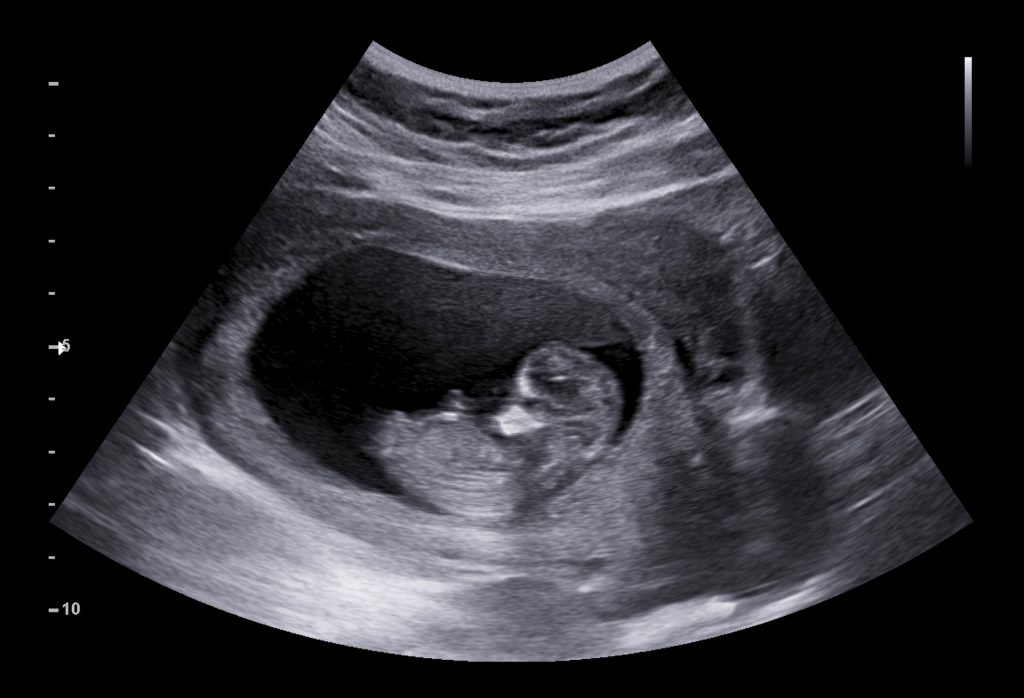
\includegraphics[width=10cm]{fetus_2D}

\section{Properties of sound}

\begin{itemize}
\item Mechanical energy in the form of \popup{high-frequency}{The
    higher the frequency the better resolution and image detail, but
    lower penetration.} (usually in the range of 2 to 18 MHz
  \cite{abdulla2025sound}) \popup{sound waves}{Sound waves are
    longitudinal preasure mechanical waves. They need a medium to
    propagate at a speed that depends on the rigidity and density of
    the medium. The typical speed in the tissue is 1540 m/s.} can be
  used to generate images of the anatomy of a patient (see Figure
  \ref{fig:sound}).
\end{itemize}
%\vspace{-2ex}
\begin{figure}[!h]
  \centering
  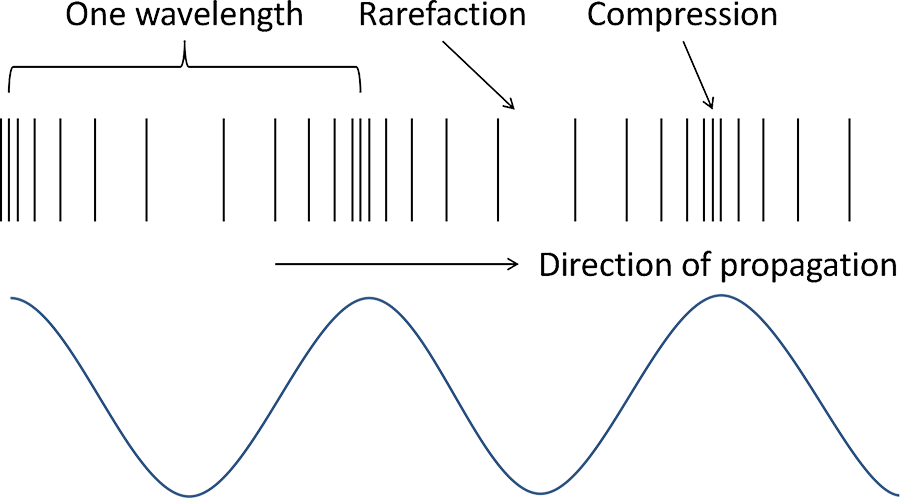
\includegraphics[width=8cm]{sound}
  \caption{Mechanical movement of the particles with the sound
    \cite{abdulla2025properties_sound}.\label{fig:sound}}
\end{figure}

\section{Echoes}
\begin{itemize}
\item \popup{(Ultra)Sound waves}{In form of decaying pulses.} pass
  through tissues, get reflected, and the returning wave (echo) is
  detected and forms the
  image\cite{bushberg2011essential,abdulla2025ultrasound_machine}. In
  \popup{B-mode}{B for Brightness (the most common ultrasound imaging
    used in medicine). There is A-Mode (A for Amplitude) that is
    mainly used in ophthalmology to investigate retinal detachment.}
  imaging, the intensity of the returning wave (echo) is represented
  as a level of brightness on the monitor to give a 2D cross-sectional
  image on the monitor \cite{abdulla2025ultrasound} (see Figure
  \ref{fig:interactions}).
\end{itemize}
%\vspace{-3ex}
\begin{figure}[!h]
  \centering
  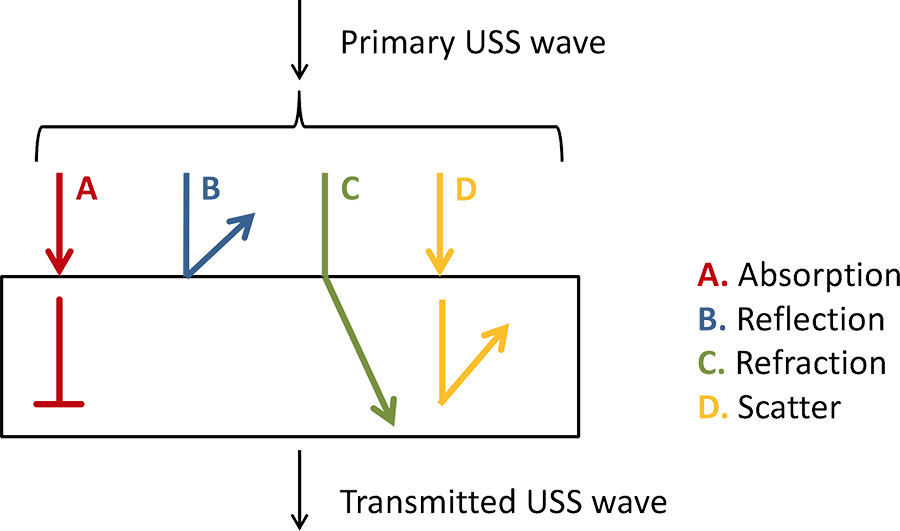
\includegraphics[width=7cm]{sound_interactions}
  \caption{Interactions of the ultrasound scan (USS) with tissue
    \cite{abdulla2025properties_sound}.\label{fig:interactions}}
\end{figure}

\section{Ultrasound imaging with flow detection}
\begin{itemize}
\item It is possible to use the \popup{M-Mode}{M for Motion.} (based
  on the Doppler effect) to detect the motion of fluids and mobile
  structures
  \cite{bushberg2011essential,abdulla2025ultrasound_machine}. Thus,
  for example, we can \popup{measure the blood flow}{Both the speed
    and direction of blood flow can be measured, and within a subarea
    of the grayscale image, a color flow display typically shows blood
    flow in one direction as red, and in the other direction as
    blue.}, displayed as color channels \cite{bushberg2011essential}
  (see Figure~\ref{fig:doppler}).
\end{itemize}
%\vspace{-4ex}
\begin{figure}[!h]
  \centering
  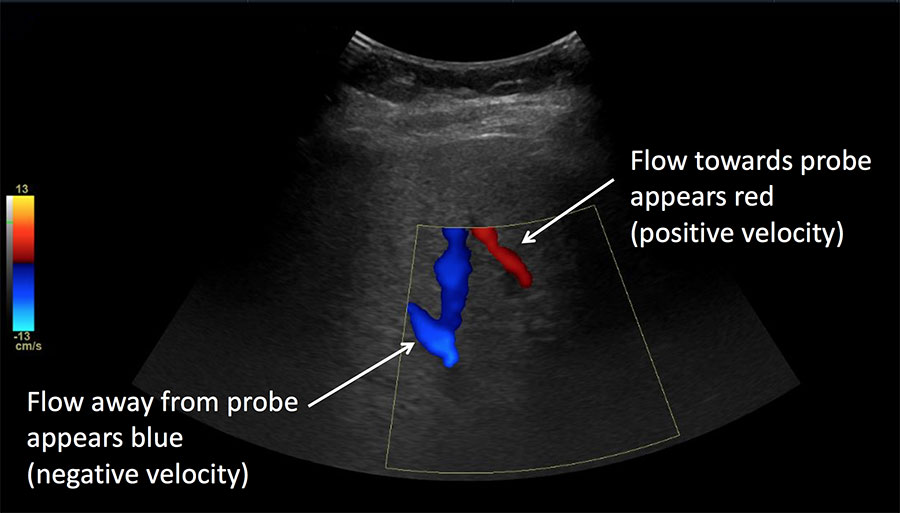
\includegraphics[width=8.0cm]{doppler}
  \caption{Ultrasound image showing flood motion
    \cite{abdulla2025ultrasound_imaging_doppler}.\label{fig:doppler}}
\end{figure}

\section{3D rendering}
\begin{itemize}
\item Ultrasound imaging is basically a \popup{2D technique}{By
    default, an ultrasound machine shows a deformed slice of the
    structure to analyze.}. However, 3D images can be generated by
  placing the known voxels in a
  \href{https://stackoverflow.com/questions/51907238/how-to-draw-a-2d-3d-grid-from-buffergeometry-in-three-js}{3D
    grid},
  \href{https://en.wikipedia.org/wiki/Trilinear_interpolation}{interpolating}
  the unknown voxels, and then,
  \href{https://en.wikipedia.org/wiki/Image_segmentation}{segmenting}
  (see Figure~\ref{fig:fetus_3D}).
\end{itemize}
%\vspace{-4ex}
\begin{figure}[!h]
  \centering
  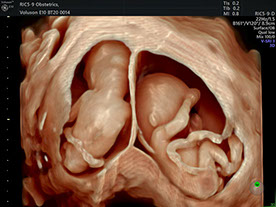
\includegraphics[width=6.0cm]{fetus_3D}
  \caption{3D ultrasound reconstruction
    \cite{fetal_diagnostic_centers}.\label{fig:fetus_3D}}
\end{figure}

\section{Artifacts}
\begin{itemize}
\item Image formation assumes that sound travels in straight lines, at
  a constant velocity, with uniform attenuation, and reflected only
  once from each interface \cite{abdulla2025ultrasound_artefacts}.
\item \popup{Artefacts}{Or artifacts, depending where you live!}
  result when the echo does not behave in this way and the system
  misinterprets it.
\end{itemize}

\section*{}
\subsection{Enhancement}
\begin{itemize}
\item Fluid filled structures are weakly
  \popup{attenuated}{Consequently, a larger proportion and greater
    amplitude beam passes through to structures in the region behind},
  and the image reconstruction algorithm interprets this as an
  \popup{increase in acoustic reflection}{The structures below show up
    brighter on the image.} (see
  Figure~\ref{fig:acoustic_enhancement}).
\end{itemize}
%\vspace{-3ex}
\begin{figure}[!h]
  \centering
  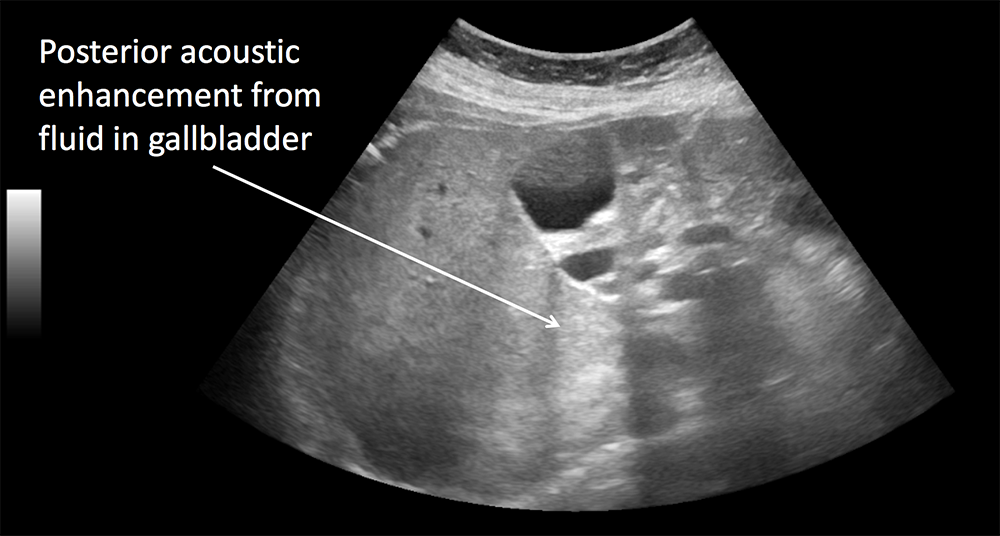
\includegraphics[width=8cm]{acoustic_enhancement}
  \caption{Acoustic enhancement artefact in ultrasound
    \cite{abdulla2025ultrasound_artefacts}.\label{fig:acoustic_enhancement}}
\end{figure}

\section*{}
\subsection{Shadowing}
\begin{itemize}
\item Hard calcific substances and soft tissue-air interfaces reflect almost all of the soundwaves. Therefore, no information is received from the area behind the structure (see
  Figure~\ref{fig:acoustic_shadowing}).
\end{itemize}
\vspace{-1ex}
\begin{figure}[!h]
  \centering
  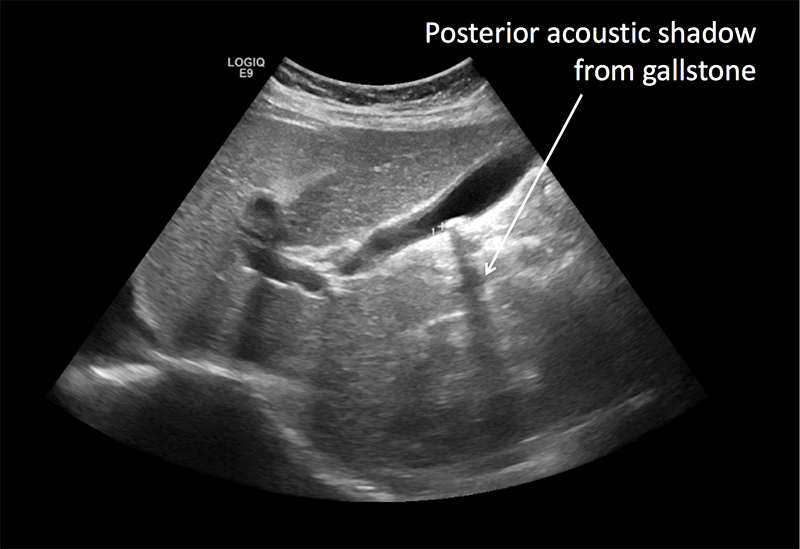
\includegraphics[width=6.5cm]{acoustic_shadowing}
  \caption{Acoustic shadowing artefact in ultrasound
    \cite{abdulla2025ultrasound_artefacts}.\label{fig:acoustic_shadowing}}
\end{figure}

\section*{}
\subsection{Reverberation}
\begin{itemize}
\item Reverberation artifacts occur when sound waves bounce back and
  forth between two surfaces, creating \popup{multiple echoes}{These
    echoes appear as parallel lines on the image, giving the
    appearance of multiple objects or structures.}. (see
  Figure~\ref{fig:acoustic_reverberation}) \cite{NysoraArtifacts}.
\end{itemize}
\vspace{-1ex}
\begin{figure}[!h]
  \centering
  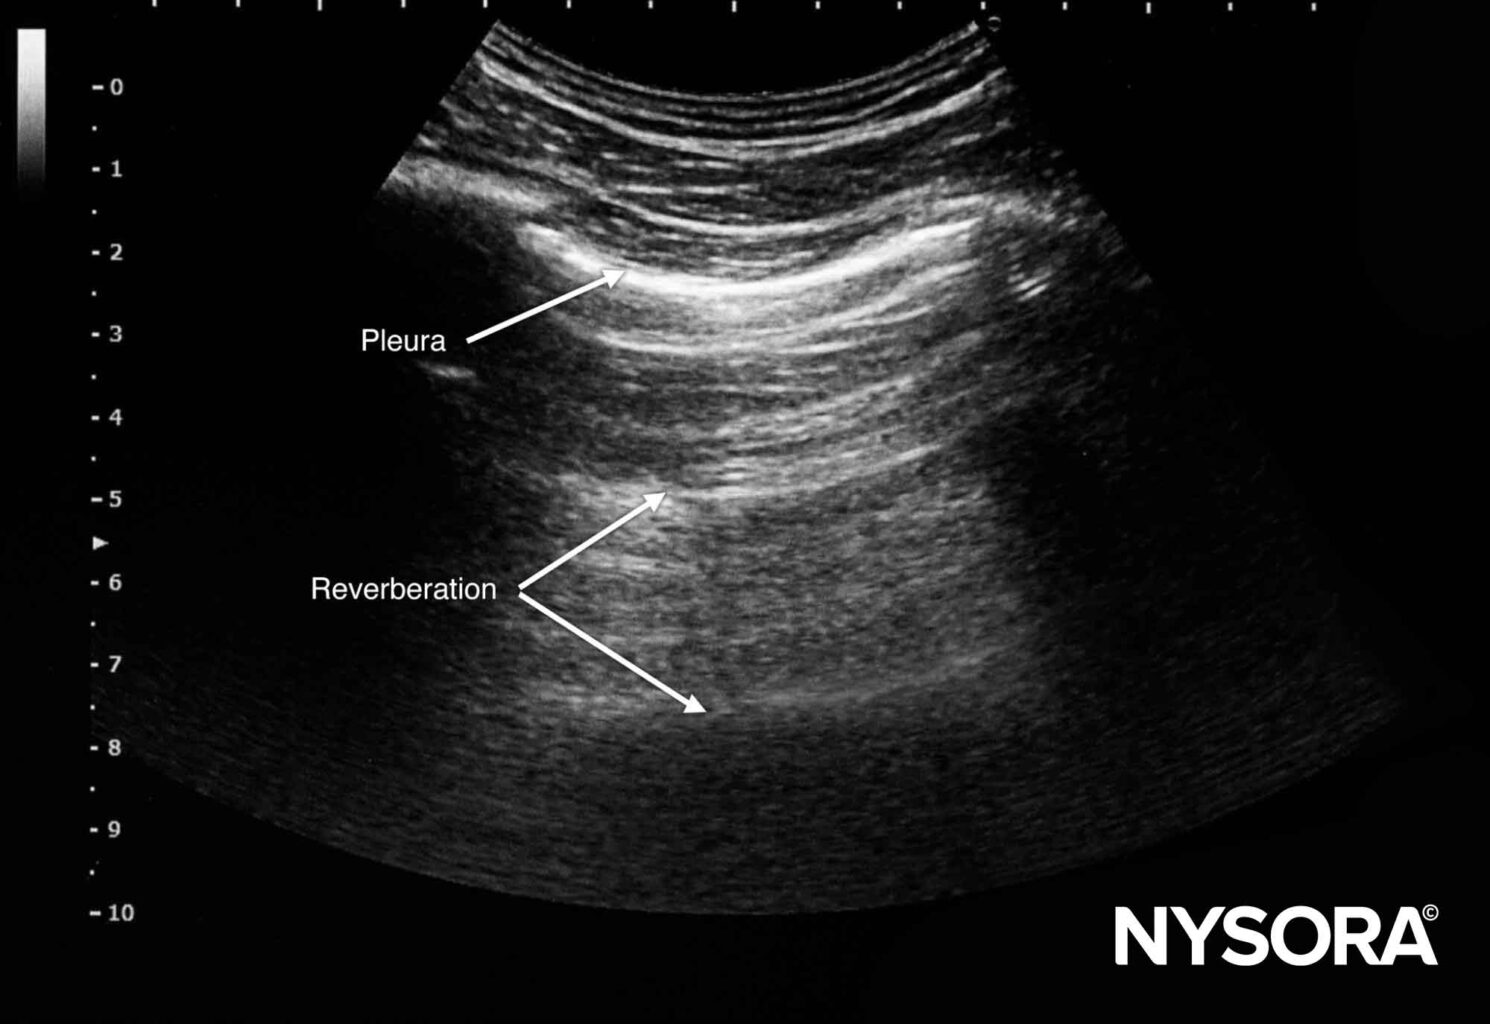
\includegraphics[width=6.5cm]{acoustic_reverberation}
  \caption{Acoustic reverberation artefact in ultrasound
    \cite{NysoraArtifacts}.\label{fig:acoustic_reverberation}}
\end{figure}

\section*{}
\subsection{Speckle}
\begin{itemize}
\item \popup{Speckle artifacts}{Also known by speckle noise.} are
  caused by the interference of sound waves with the echoes, resulting
  in a granular or \popup{speckled appearance of the image}{These
    artifacts can make it difficult to distinguish between small
    structures, such as blood vessels.}  \cite{NysoraArtifacts} (see
  Figure~\ref{fig:acoustic_speckle}).
\end{itemize}
\vspace{-2ex}
\begin{figure}[!h]
  \centering
  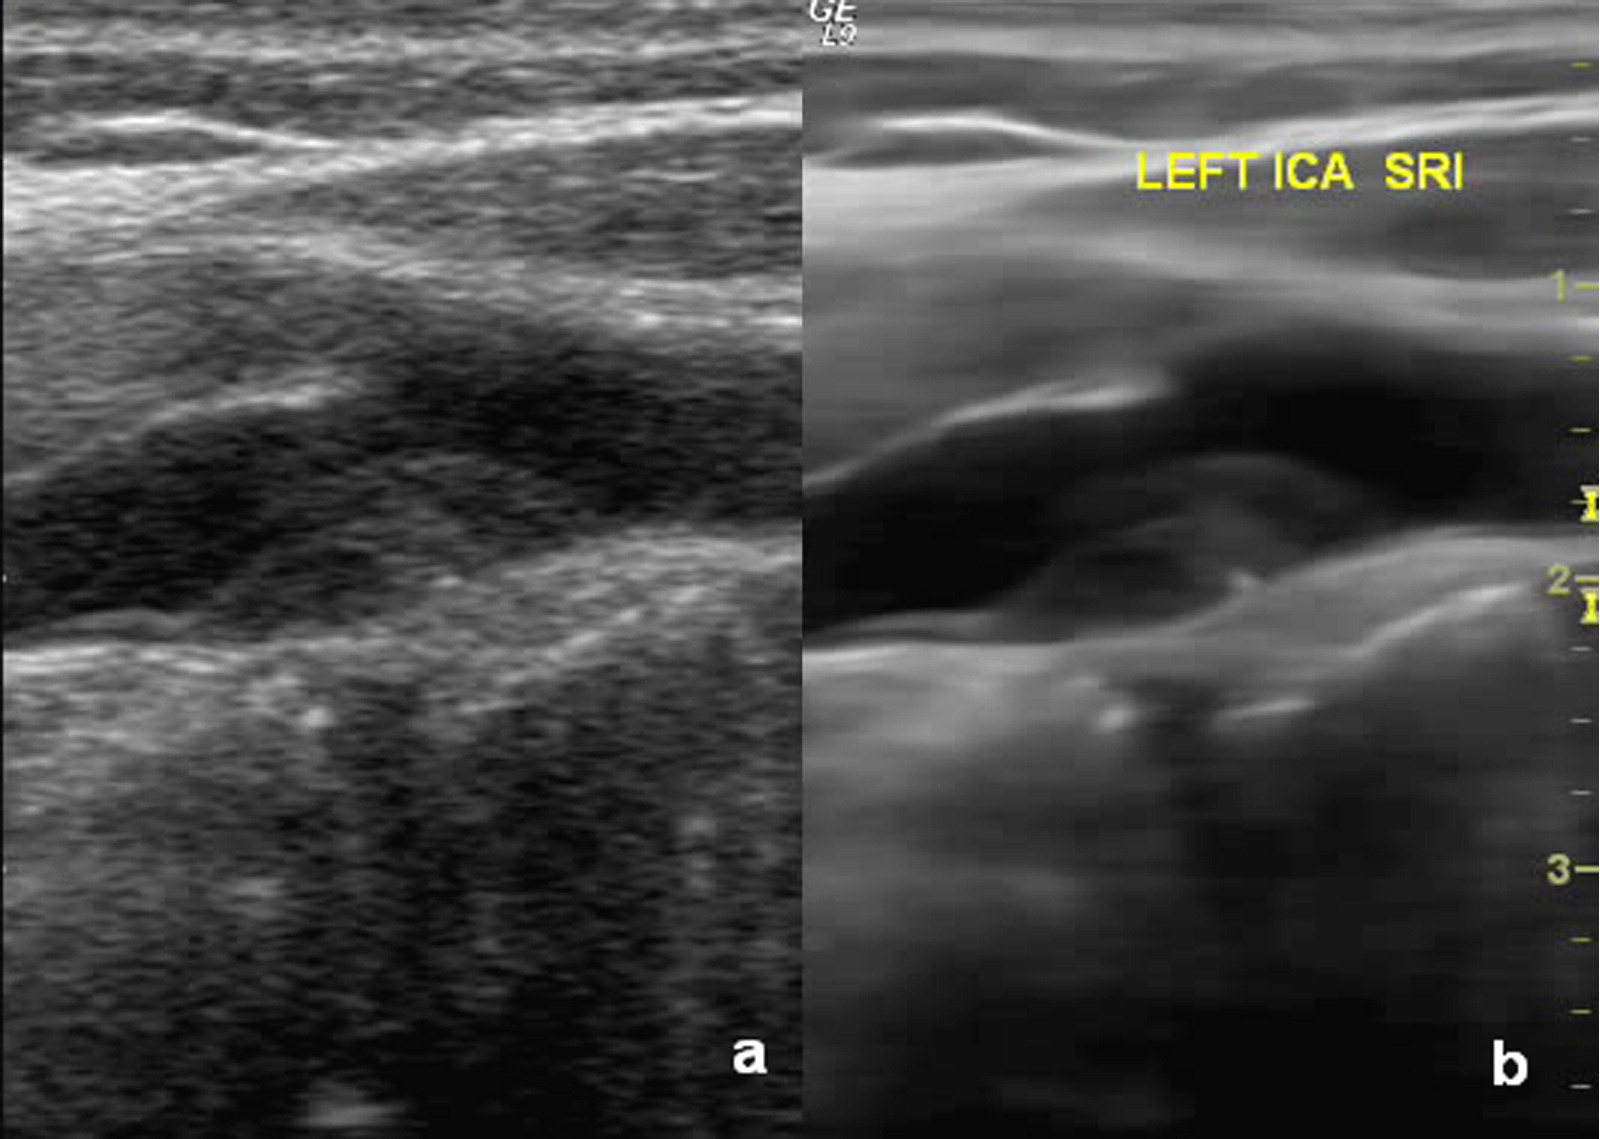
\includegraphics[width=6.5cm]{acoustic_speckle}
  \caption{Speckle noise in ultrasound
    \cite{LIASIS2008427}.\label{fig:acoustic_speckle}}
\end{figure}

\section*{}
\begin{itemize}
\item Speckle is usually modeled as \popup{multiplicative
    noise}{Multiplicative noise is proportional to the intensity of
    the clean signal.}. Its amplitude (which depends on the clean
  signal) follows a
  \href{https://en.wikipedia.org/wiki/Rayleigh_distribution}{Rayleigh
    distribution}, and its phase is
  \href{https://en.wikipedia.org/wiki/Discrete_uniform_distribution}{uniformly
    distributed}.

\item If multiple images are taken (changing the angle and
  orientation) and averaged \emph{spatial compounding}, speckle noise
  dimishes following a
  \href{https://en.wikipedia.org/wiki/Gamma_distribution}{Gamma
    distribution} \cite{bushberg2011essential}.
\end{itemize}

%\chapter{Radiography}
\vspace{-47ex}\hspace{38ex}
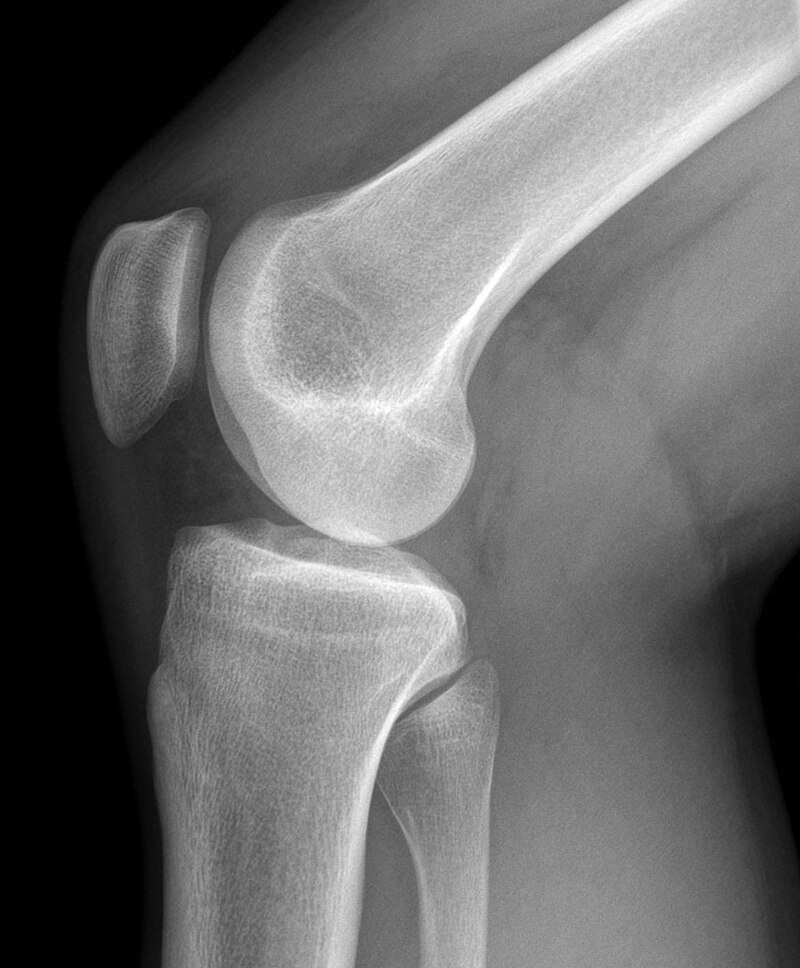
\includegraphics[width=10cm]{Knie-roentgen-r-seite} % https://upload.wikimedia.org/wikipedia/commons/thumb/8/89/Knie-roentgen-r-seite.jpg/800px-Knie-roentgen-r-seite.jpg

\section{X-ray and radiography}
\begin{itemize}
\item Radiography (X-ray 2D \popup{projection}{Radiography is also a
    projection imaging modality, meaning that each point on the image
    corresponds to information along a straight line through the
    patient}) is a transmission imaging modality where X-rays are
  emitted from a \popup{source}{An X-rays generator.}, pass through
  the patient, and are detected on the other side using a flat
  (usually \popup{digital TFT}{In digital X-ray detectors, a TFT array
    is used to read out electrical charges generated by the impact of
    the X-rays.}) detector (see
  Fig.~\ref{fig:projectional_radiography}).
\end{itemize}
\vspace{-4ex}
\begin{figure}[!h]
  \centering
  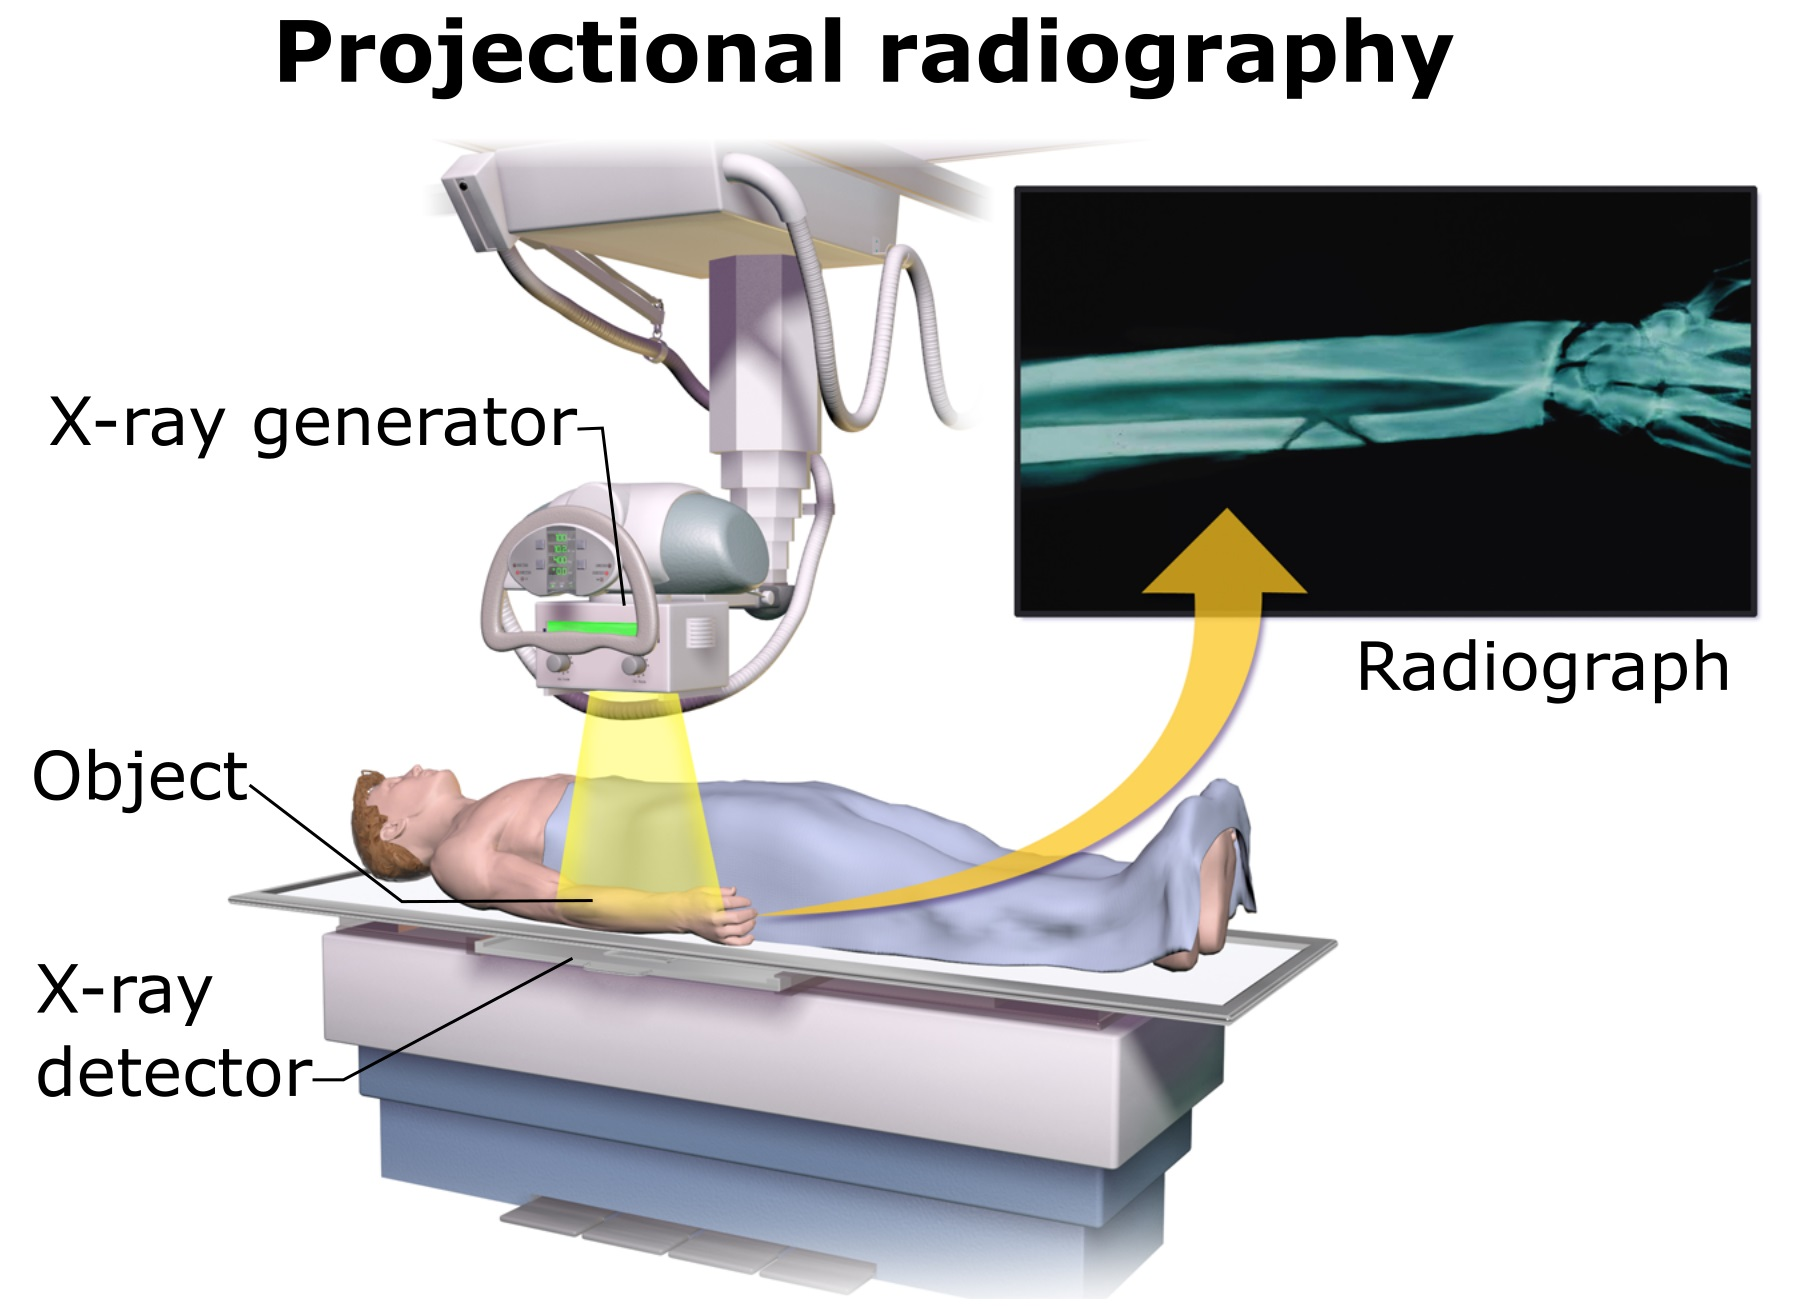
\includegraphics[width=6cm]{Projectional_radiography_components}
  \caption{Acquisition of projectional radiography, with an X-ray generator and a detector
    \cite{Wikipedia_X-ray_machine}.\label{fig:projectional_radiography}}
\end{figure}

\section{Transmission and attenuation}
\begin{itemize}
\item The X-ray attenuation of different tissues (e.g., bone, soft
  tissue, air) modify the homogeneous distribution of X-rays that
  enters the patient X-ray, forming the image in the detector
  \cite{bushberg2011essential} (see
  Fig.~\ref{fig:Attenuation-of-X-rays}).
\end{itemize}
\vspace{-3ex}
\begin{figure}[!h]
  \centering
  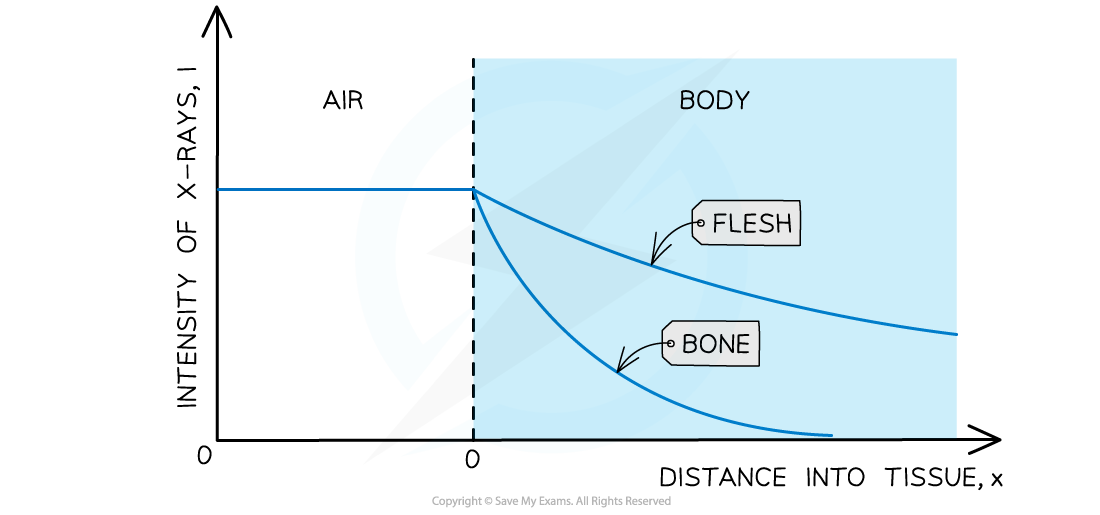
\includegraphics[width=9cm]{Attenuation-of-X-rays}
  \caption{Intensity-distance graph of X-rays for air and body
    \cite{Attenuation_X-rays}.\label{fig:Attenuation-of-X-rays}}
\end{figure}

\section{\glsentrylong{LAC} (\glsentryshort{LAC})}
\begin{itemize}
\item The X-rays are
  exponentially attenuated when they travel across the tissues \cite{wikipedia_LAC}.
\item To simplify numerical analysis and processing, we don't work
  directly with the attenuation coefficients but with the \glspl{LAC}, which
  are obtained applitying a logarithm operation.
\item For example, the numerical values used in
  Section~\ref{sec:FBP_example} are the result of computing the
  logarithm of the \popup{measured}{Returned by the detector.}
  attenuation coefficients.
\end{itemize}

\section{Why are we ``transparent''?}
\begin{itemize}
\item The \popup{fast ondulatory movement of X-ray-photons}{From 30
    petahertz (PHz)}{3x10$^{16}$ Hz.} to \popup{30 exahertz
    (EHz)}{3x10$^{19}$ Hz} makes them capable of \popup{penetrating
    soft tissues}{The higher the frequency of the X-rays photons, the
    higher their energy and the higher their penetration capability.}.
\end{itemize}
\vspace{-4ex}
\begin{figure}[!h]
  \centering
  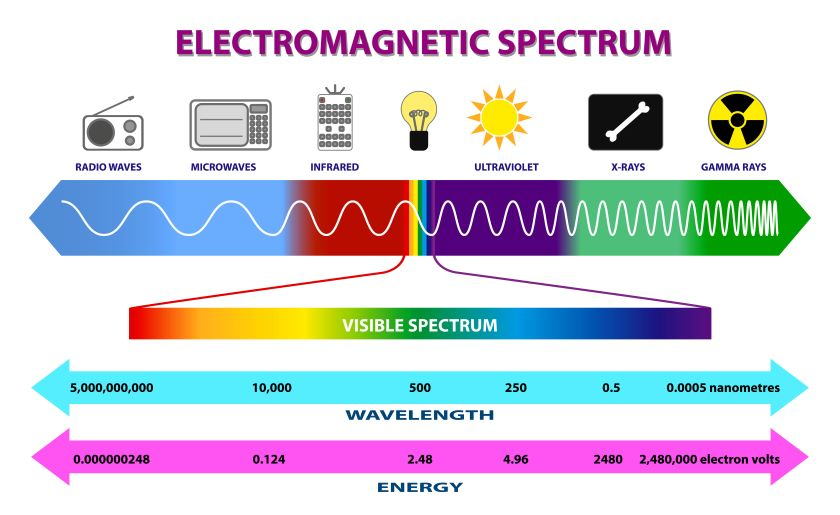
\includegraphics[width=8cm]{electromagnetic-spectrum}
  \caption{The electromagnetic spectrum
    \cite{X-rays_in_spectrum}.\label{fig:X-rays_in_spectrum}}
\end{figure}

\section{Ionization and biologic damage}
\begin{itemize}
\item X-rays are a form of \popup{ionizing radiation}{An ionizing
    radiation is capable of removing electrons from atoms or
    molecules, a process known as ionization (when an atom or molecule
    loses or gains electrons, it acquires a net electrical charge and
    becomes an ion).} (see Fig.~\ref{fig:ionization}), creating
  \popup{free radicals}{A free radical is an atom or molecule that has
    an unpaired electron in its outer shell. Because electrons prefer
    to exist in pairs, this unpaired electron makes the free radical
    highly unstable and very reactive.}.
\end{itemize}
\vspace{-3ex}
\begin{figure}[!h]
  \centering
  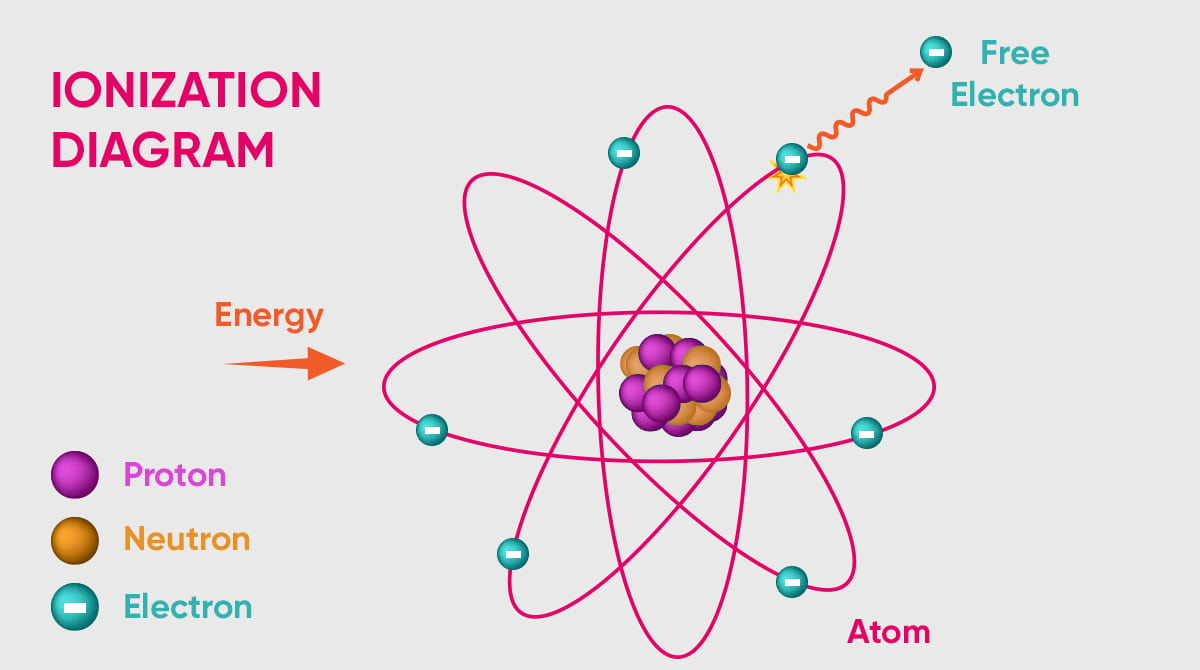
\includegraphics[width=8cm]{ionization-diagram}
  \caption{Ionization
    \cite{Perakende_ionization}.\label{fig:ionization}}
\end{figure}

\begin{itemize}
\item Free radicals are extremely reactive and can interact with
  biomolecules. This can produce a list of effects
  \cite{bushberg2011essential}:
  \begin{enumerate}
  \item \textbf{Short-term effects} (usually under high doses):
    \href{https://en.wikipedia.org/wiki/Radiation_burn}{burns},
    sickness.
  \item \textbf{Long-term effects}:Damage to DNA, could suffer
    \popup{mutations}{Although heavily irradiated cells often die
      during mitosis, preventing the propagation of seriously
      defective cells, damage to DNA at locations responsible for
      controlling cell division (e.g., oncogenes or tumour suppressor
      genes) could potentially lead to the formation of a tumour or
      cancer}, and \popup{tissue disfunction}{If there is ellular
      dysfunction, tissues can lose function and finally generate
      organ failure.}.
  \end{enumerate}
\end{itemize}

\section{Artifacts}
\begin{itemize}
\item In radiology, artifacts come from hardware failure, operator
  error (including the interaction/control with/of the patient) and
  software (post-processing) artifacts.
\item Only in digital radiology.
\end{itemize}

\section*{}
\subsection{Motion blur}
\vspace{-4ex}
\begin{figure}[!h]
  \centering
  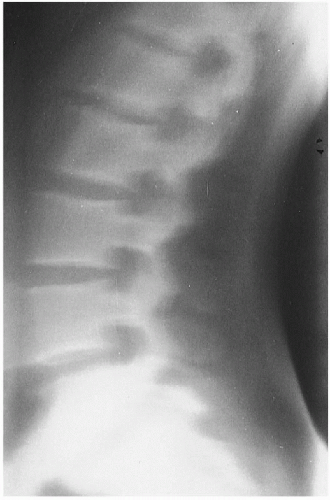
\includegraphics[width=3.5cm]{motion_blur_2}
  \caption{The image unsharpness was caused by patient movement
    \cite{radiology_key}.\label{fig:motion_blur}}
\end{figure}

\section*{}
\subsection{Static electricity}
\vspace{-3ex}
\begin{figure}[!h]
  \centering
  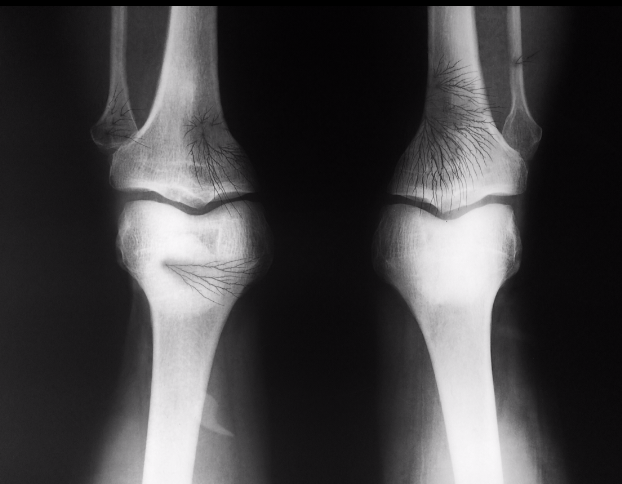
\includegraphics[width=7cm]{static-electricity}
  \caption{\cite{radiopaedia}.\label{fig:static_electricity}}
\end{figure}

\section*{}
\subsection{Dead pixel}
\vspace{-3ex}
\begin{figure}[!h]
  \centering
  \begin{tabular}{cc}
    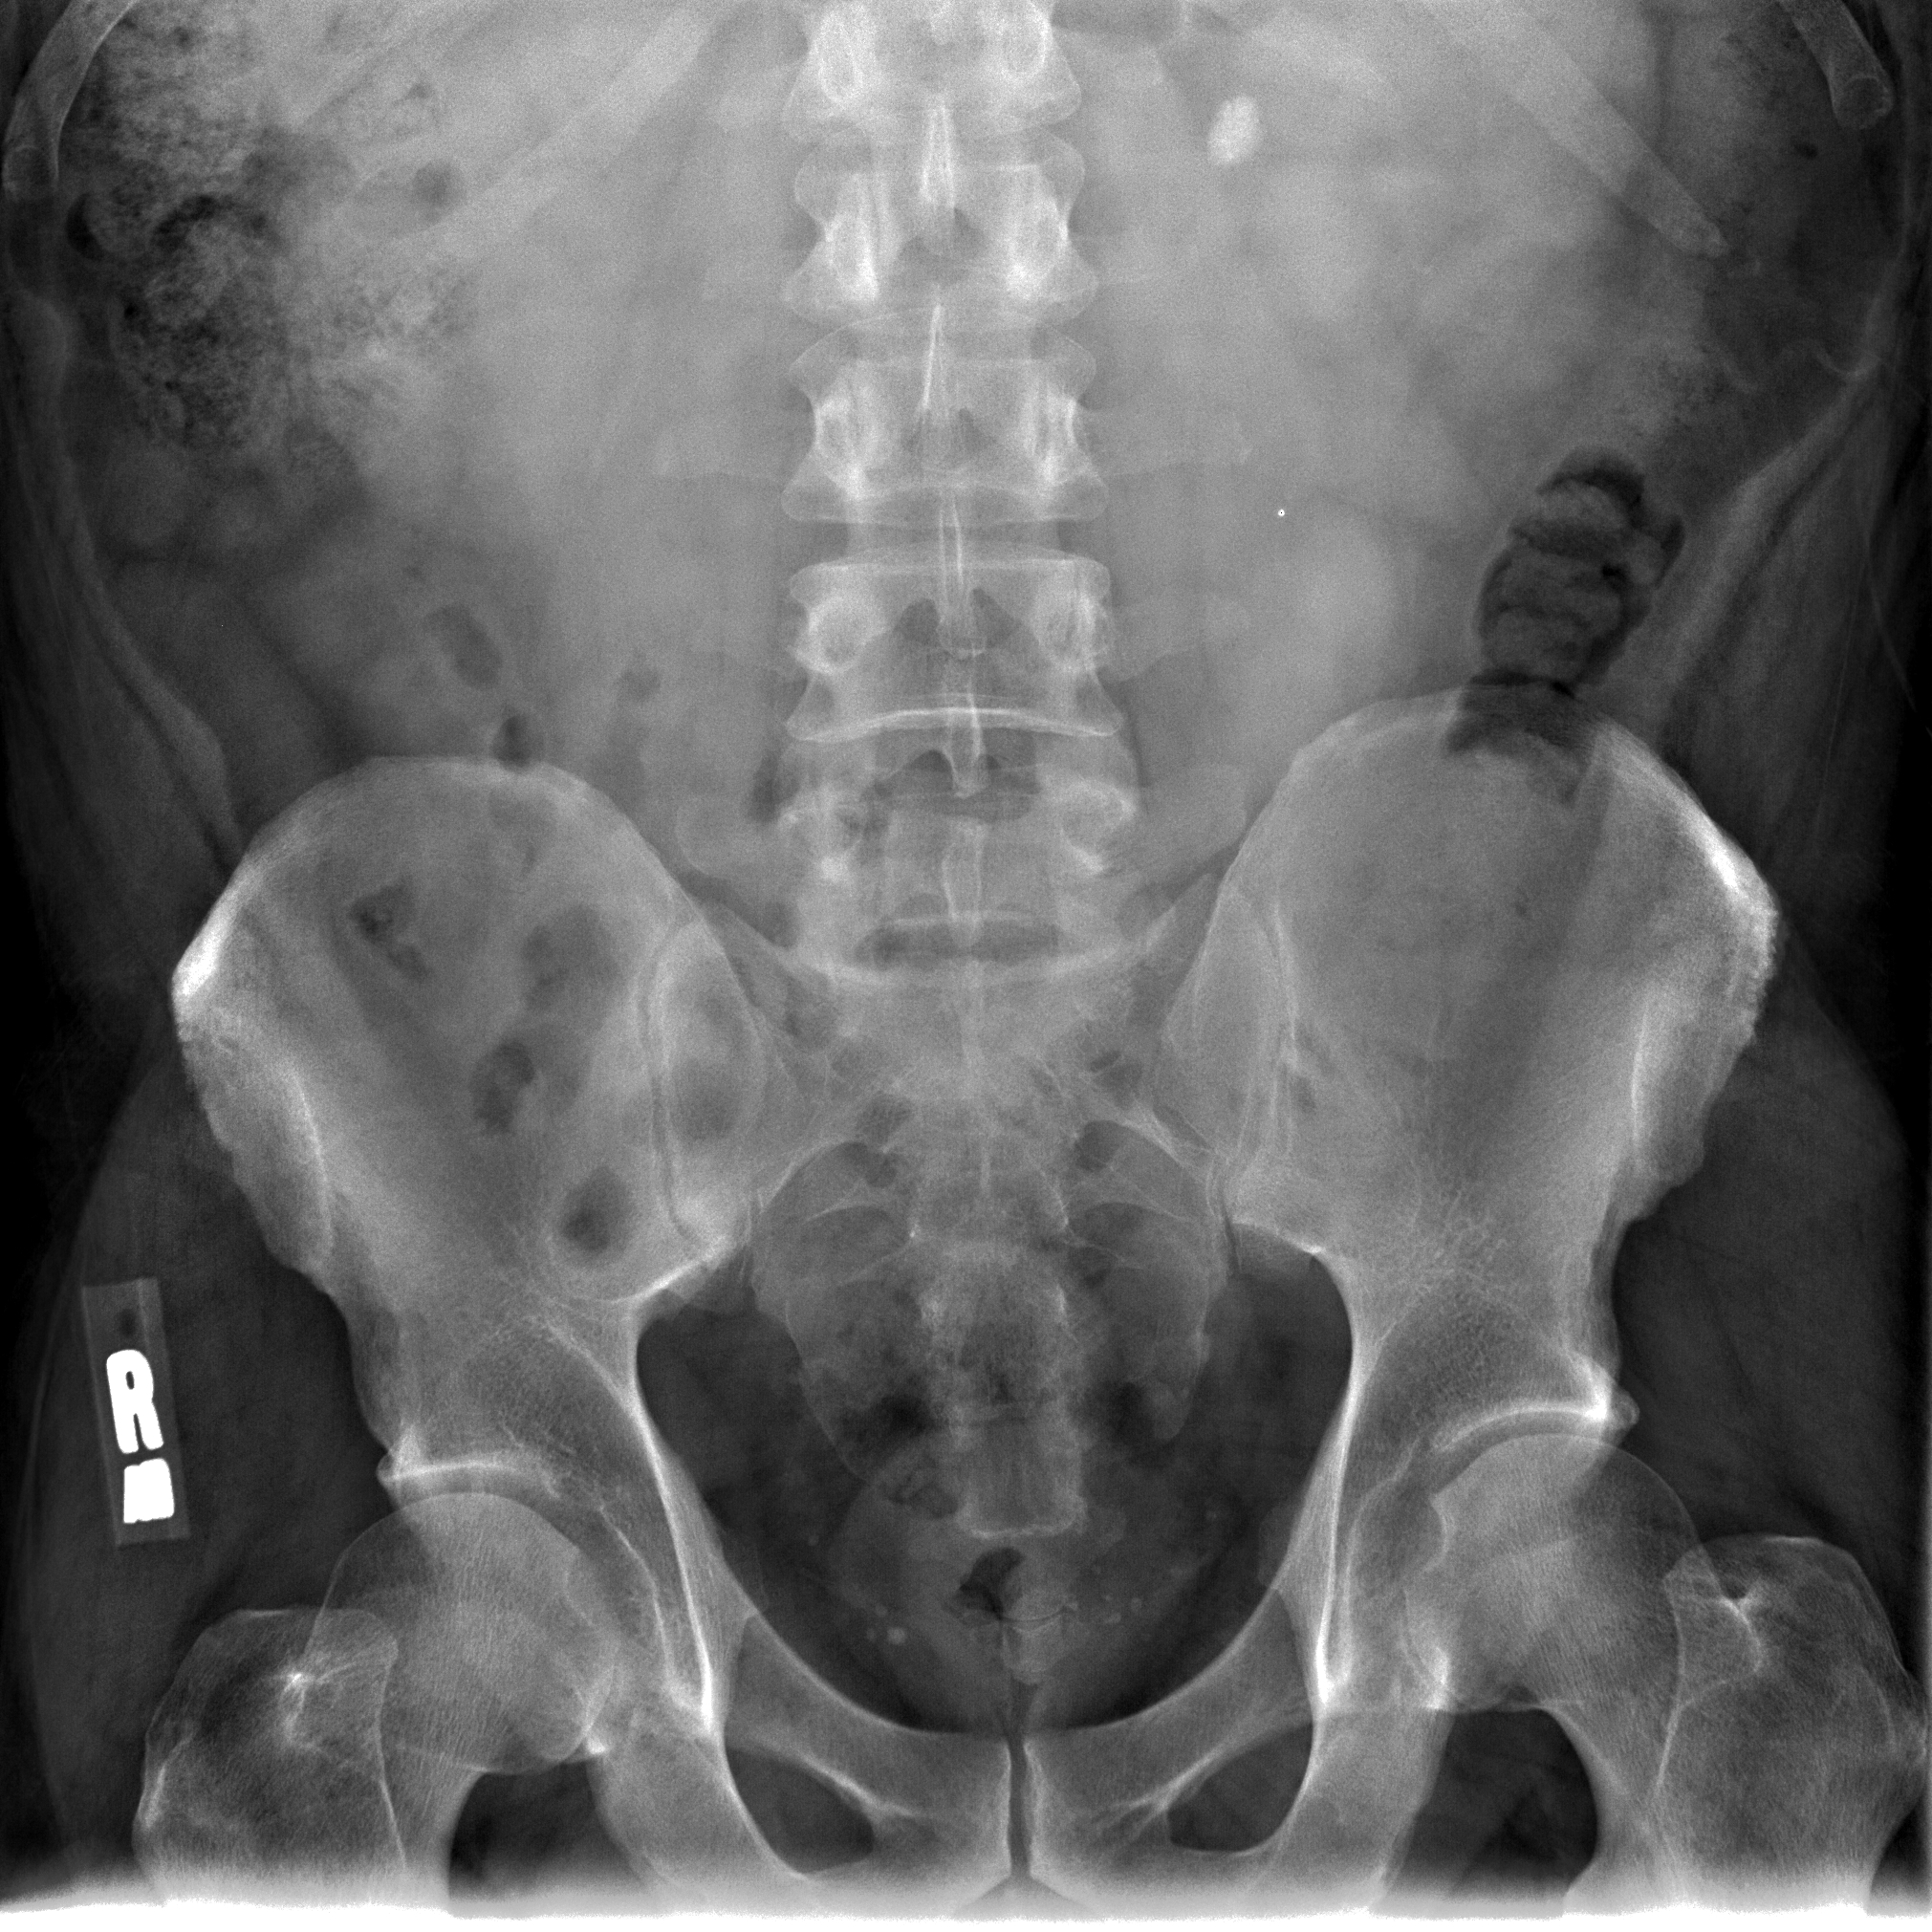
\includegraphics[width=5cm]{dead-pixel-artifact_frontal} &
                                                               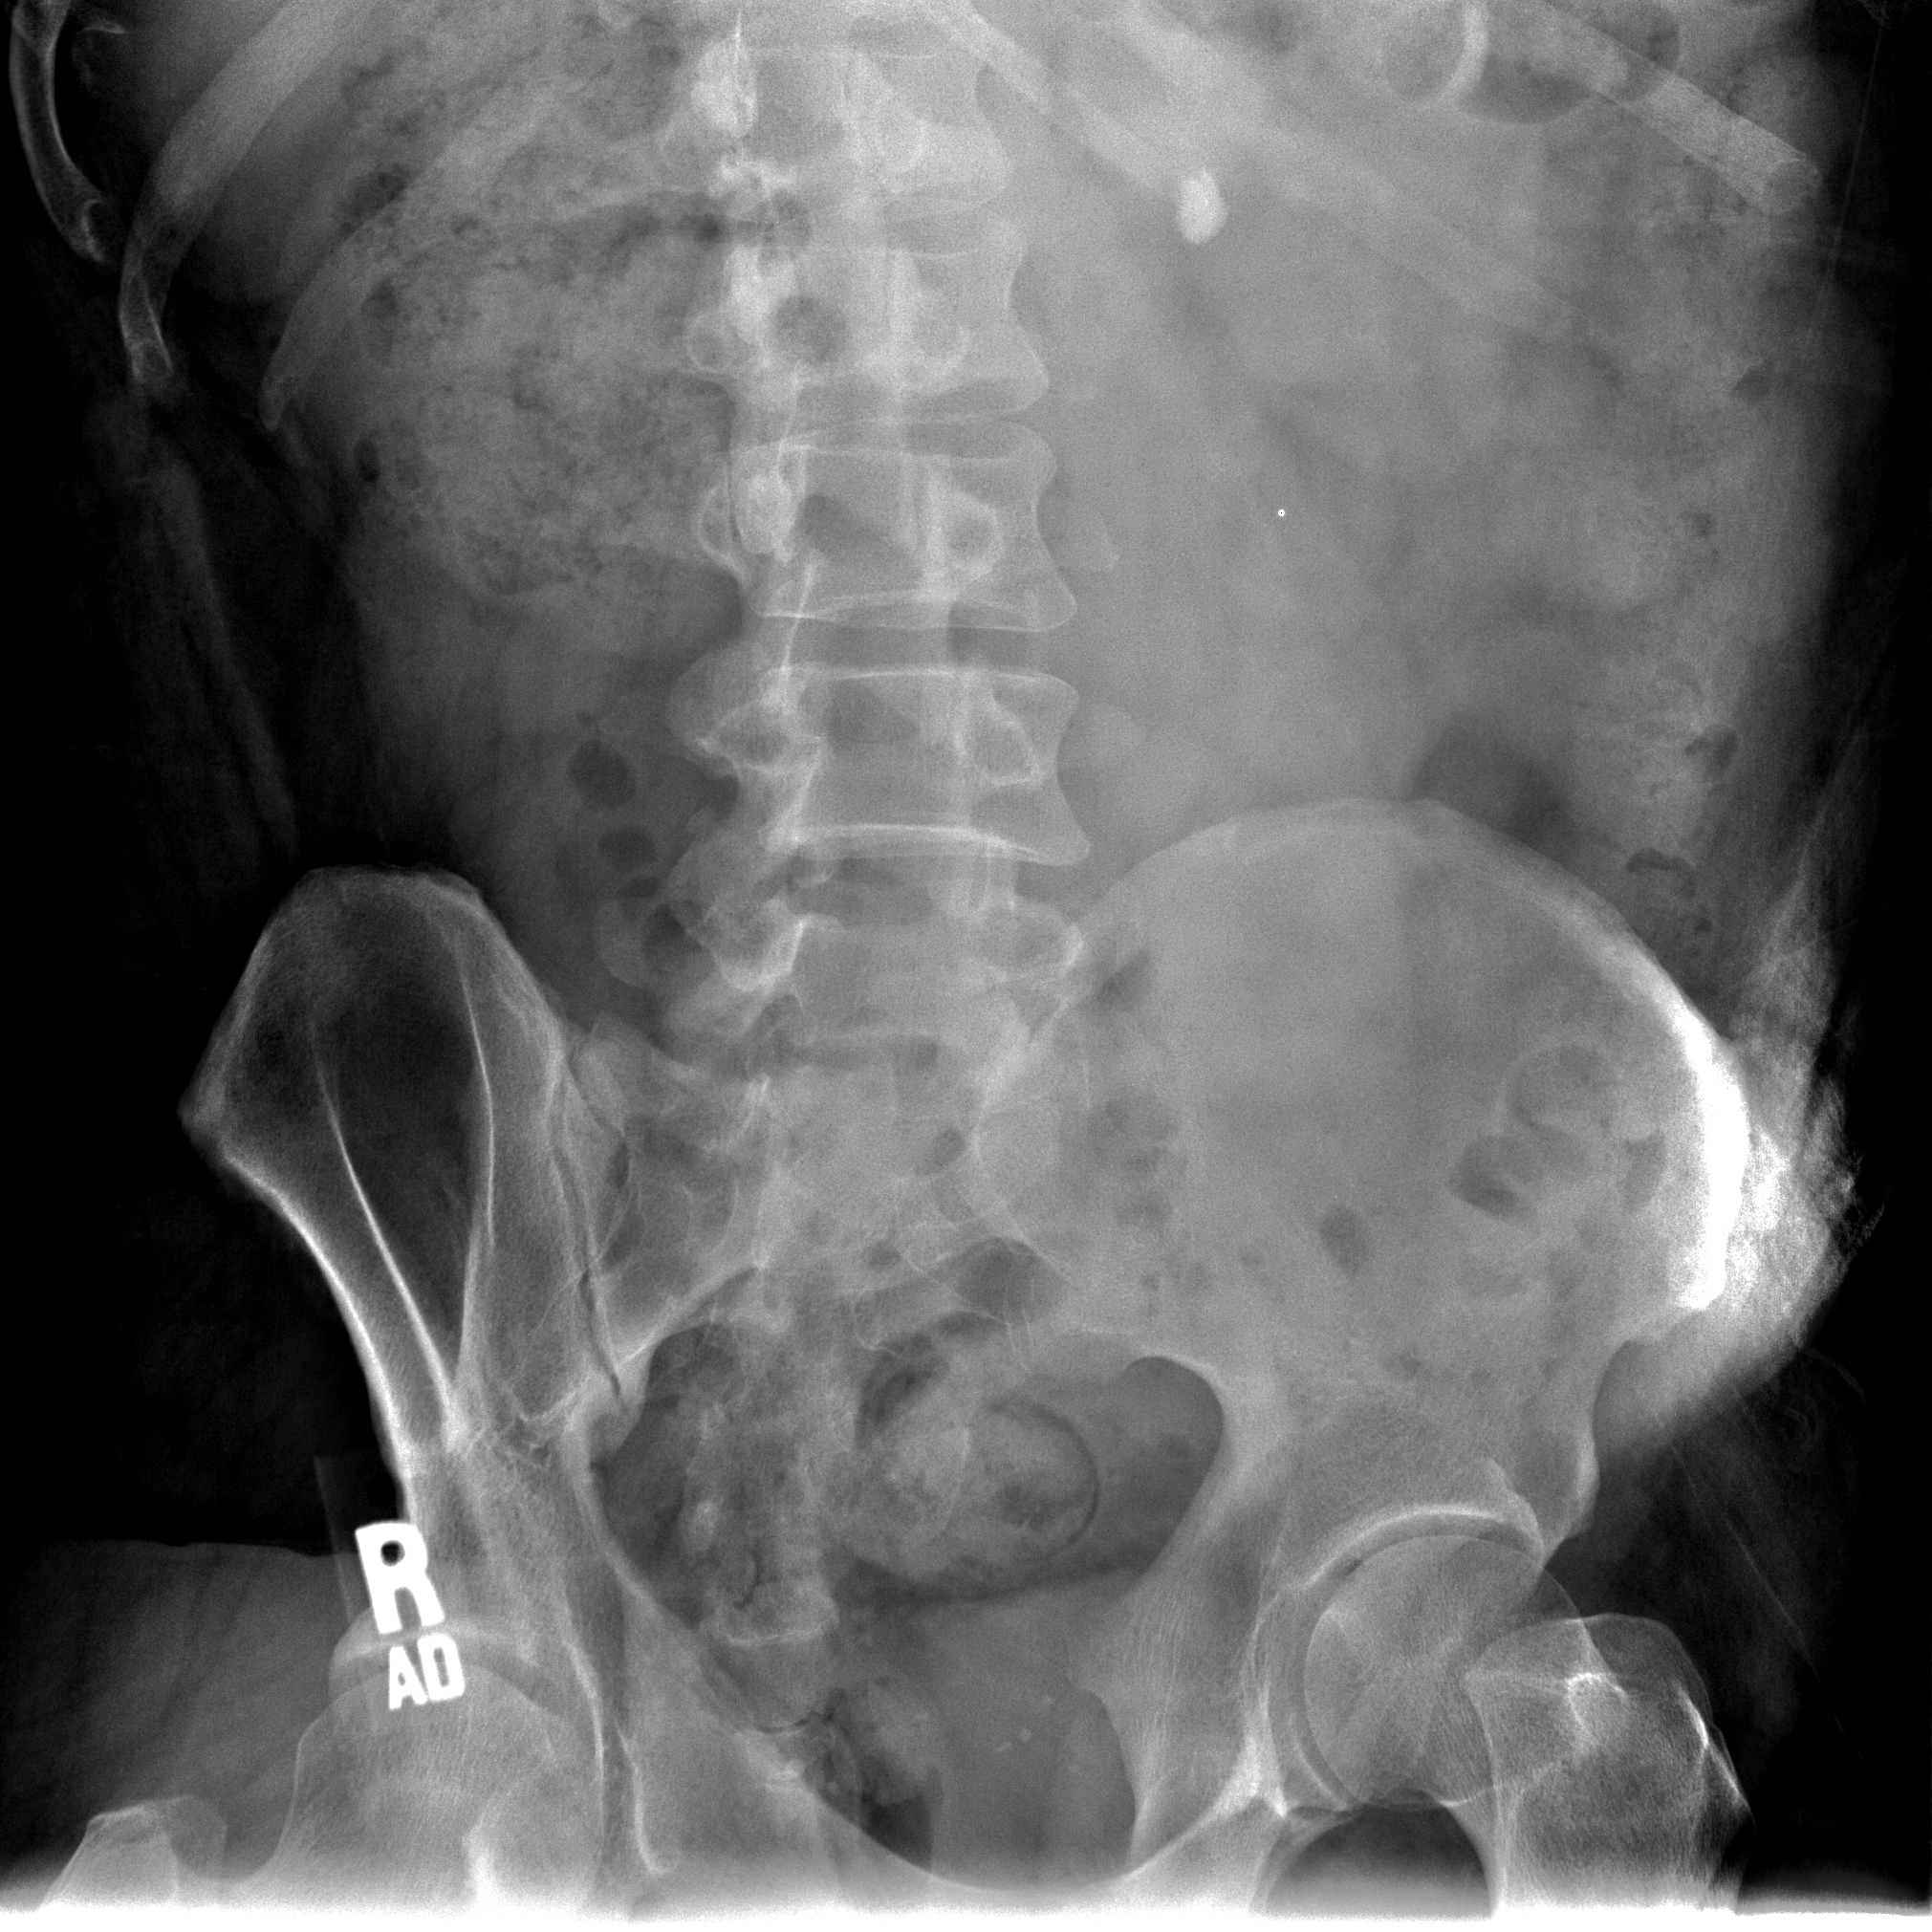
\includegraphics[width=5cm]{dead-pixel-artifact_oblique}
  \end{tabular}                                                
  \caption{Dead pixels are always white. \cite{radiopaedia}.\label{fig:dead_pixel}}
\end{figure}

\section*{}
\subsection{Under- and over-exposure}
\begin{itemize}
\item In digital radiology (down), the detector always generates a good contrast.
\item The main drawback is that, under-exposure usually have more noise.
\end{itemize}
\vspace{-4ex}
\begin{figure}[!h]
  \centering
    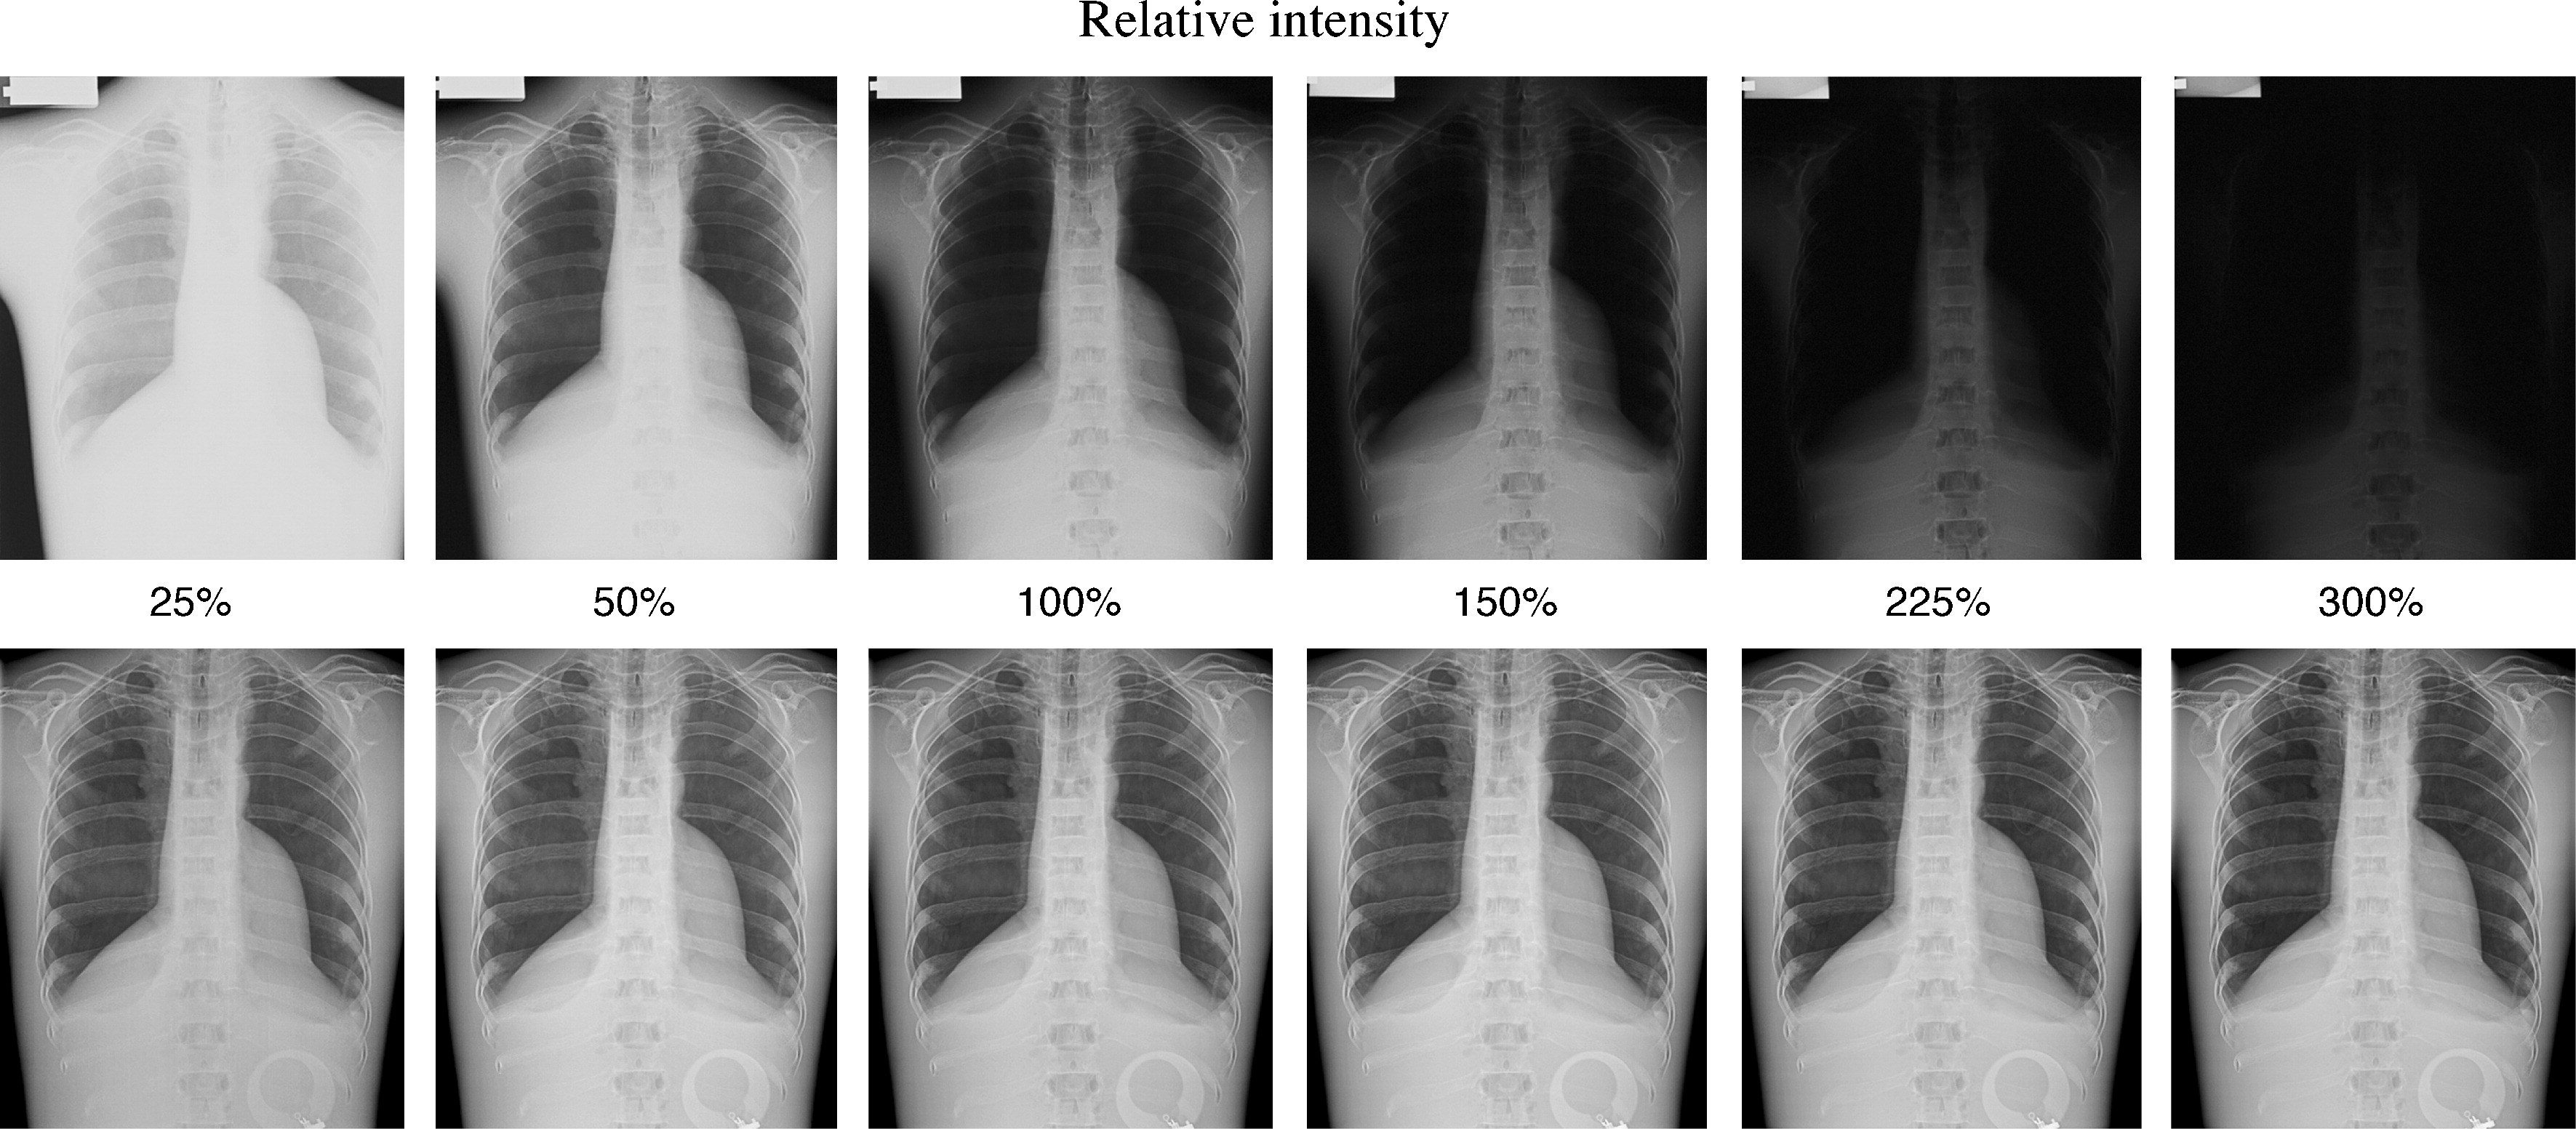
\includegraphics[width=9cm]{X-ray_exposure}
    \caption{Exposure impact (up: analog, down: digital)
      \cite{VELDKAMP2009209}.\label{fig:exposure}}
\end{figure}

\section{Mammography}
\begin{itemize}
\item Mammography is the 2D X-rays projection\\ of the breast
  \cite{bushberg2011essential}.
\item Makes use of much lower x-ray energies\\ than general purpose
  radiography.
\end{itemize}
\vspace{-20ex}
\begin{figure}[!h]
  \begin{flushright}
    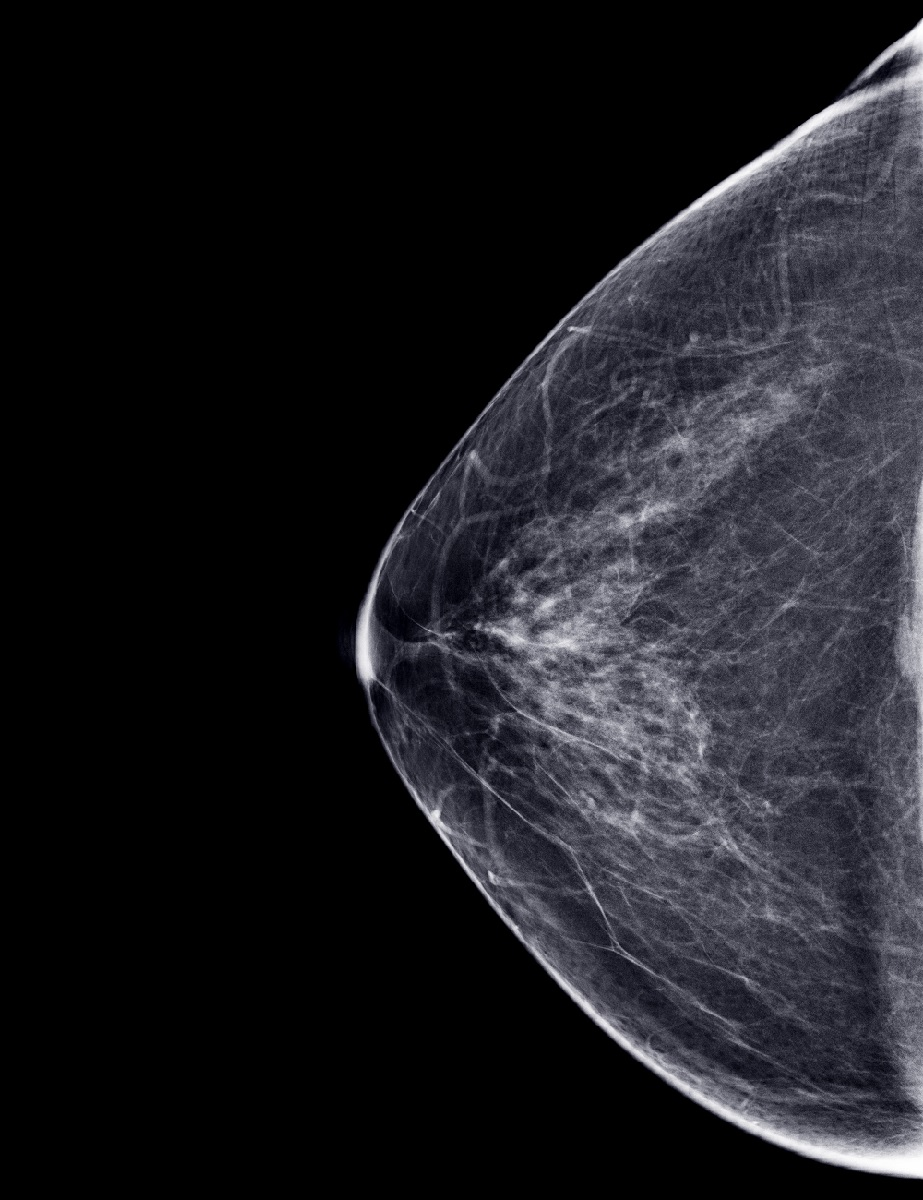
\includegraphics[width=4.5cm]{normal_mammogram}
    \end{flushright}
    \caption{Mamogram \cite{CDC_mammograms}.\label{fig:mamogram}}
\end{figure}

\section{Fluoroscopy}
\begin{itemize}
\item A fluoroscope produces real-time X-ray images with high temporal
  resolution (e.g., 30 frames per second), allowing continuous motion
  viewing, useful for \popup{interventional procedures}{Fluoroscopy is
    used for positioning catheters in arteries, visualizing contrast
    agents in the \gls{GI} tract, and for other medical applications
    such as invasive therapeutic proce- dures where real-time image
    feedback is necessary. It is also used to make x-ray movies of
    anatomic motion, such as of the heart or the esophagus.}
  \cite{bushberg2011essential}.
\item Compared to ``one-shot'' radiography, the images are more noisy.
\item
  \href{https://en.wikipedia.org/wiki/Fluoroscopy#/media/File:Normal_barium_swallow_animation.gif}{Swallowing
    of varium} \cite{Wikipedia_Fluoroscopy}.
\end{itemize}

\section{Quantum noise}
\begin{itemize}
\item Quantum noise is the most common noise in X-rays imaging.
\item It is directly related to photon counting (fewer photons
  $\rightarrow$ more noise).
\item More evident (lower \gls{SNR}) at low radiation doses.
\end{itemize}
\vspace{-4ex}
\begin{figure}[!h]
  \centering
    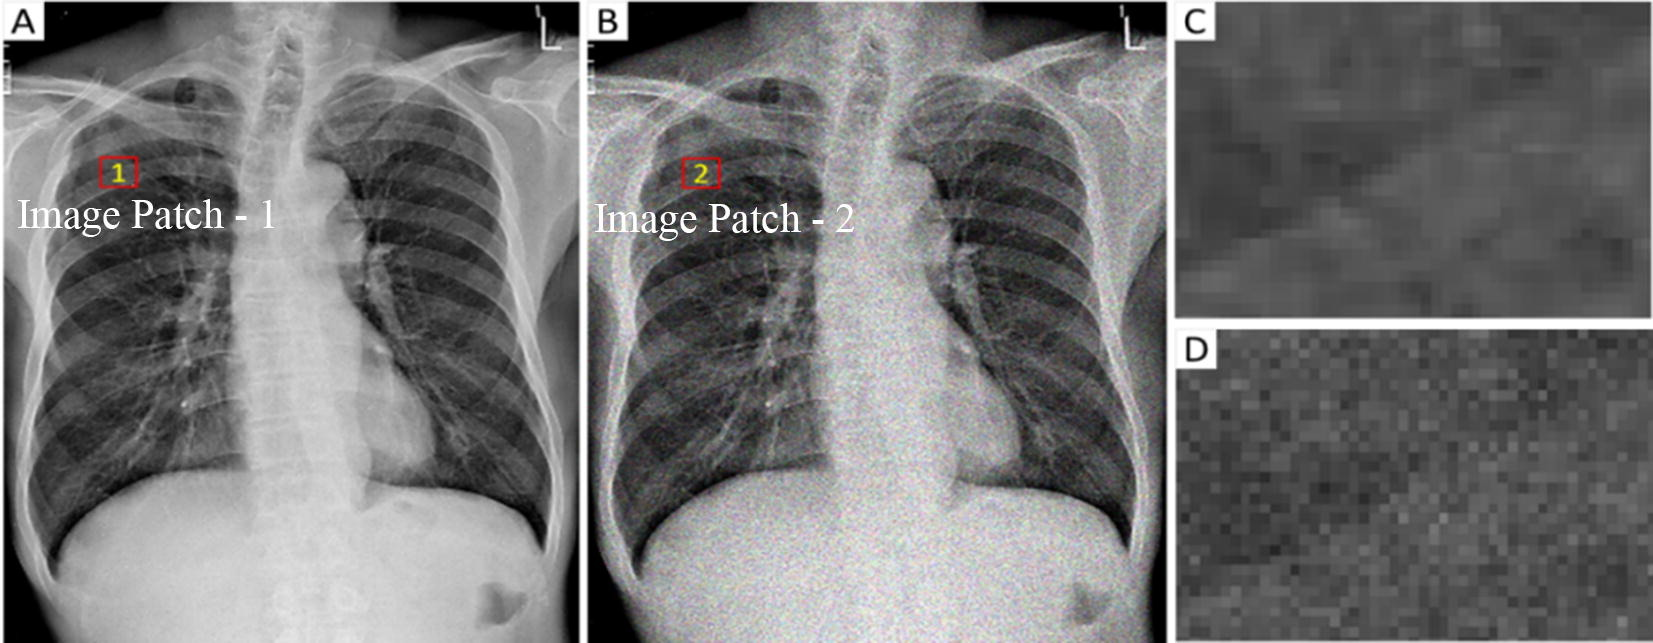
\includegraphics[width=10cm]{quantum_noise_X-rays}
    \caption{Quantum noise in radiology
      \cite{CHANDRA2020107426}.\label{fig:quantum_noise_X-rays}}
\end{figure}

\label{sec:radiography_quantum_noise}
\begin{itemize}
\item The amplitude of quantum noise depends on the (clean) signal amplitude.  
\item On average, quantum noise appears on all the frequencies and is typically \href{https://en.wikipedia.org/wiki/Colors_of_noise}{colored}.
\end{itemize}
\vspace{-4ex}
\begin{figure}[!b]
  \centering
    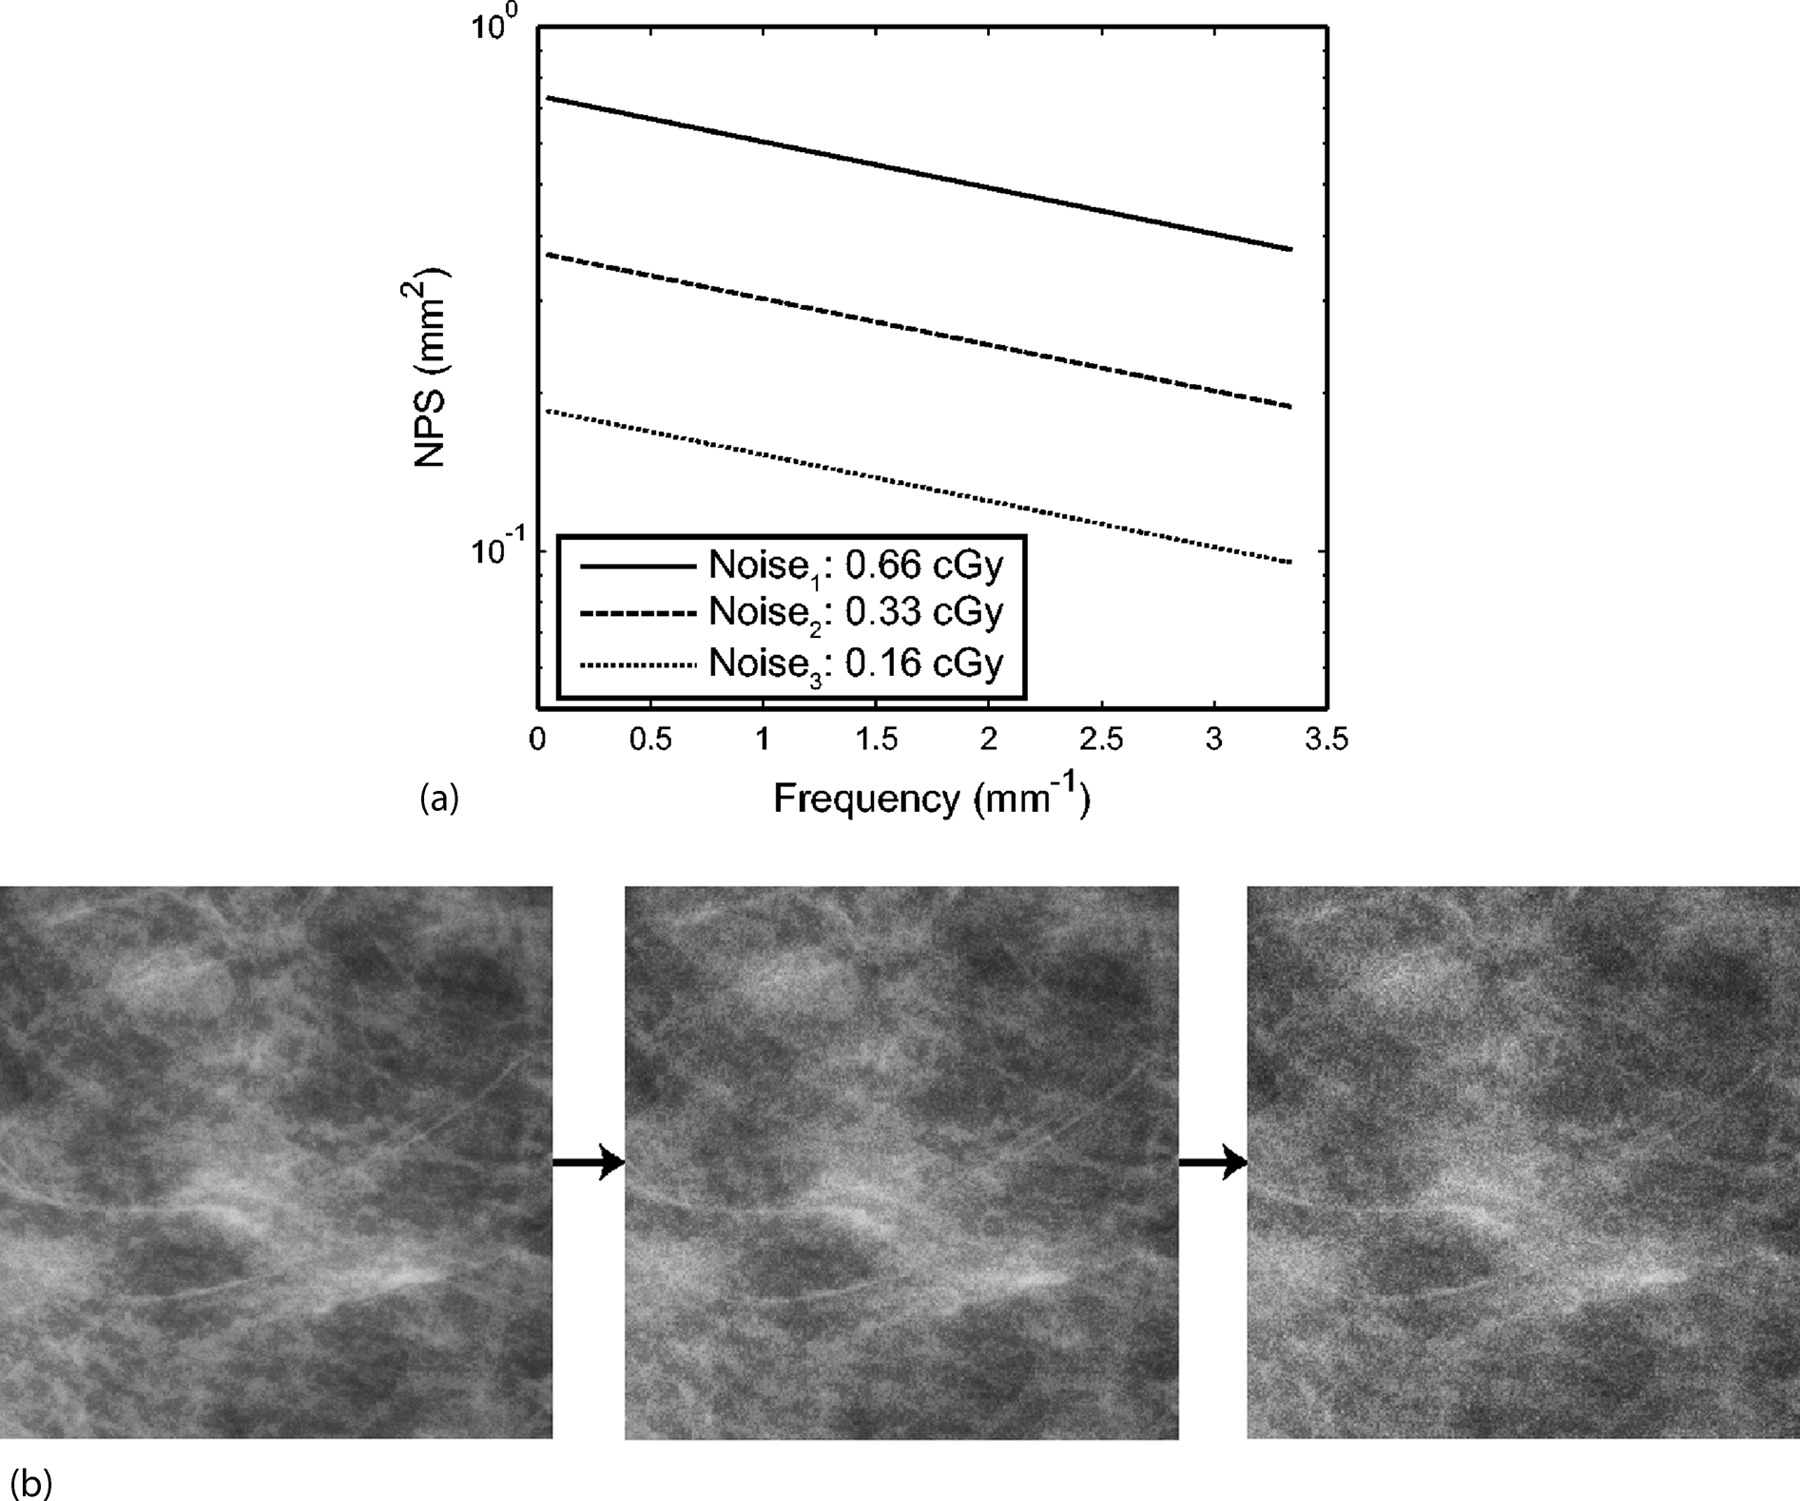
\includegraphics[width=6cm]{quantum_noise_mammography}
    \caption{Average quantum noise spectrum (up), some examples in mammograms (below) 
      \cite{saunders2007does}.\label{fig:quantum_noise_X-rays_spectrum}}
\end{figure}

%\chapter{Computed Tomography (CT)}

CT images are produced by passing x-rays through the body at a large
number of angles, by rotating the x-ray tube around the body. A
detector array, opposite the x-ray source, collects the transmission
projection data. The numerous data points collected in this manner are
synthesized by a computer into tomographic images of the patient. The
term tomography refers to a picture (graph) of a slice (tomo). The
advantage of CT over radiography is its ability to display
three-dimensional (3D) slices of the anatomy of interest, eliminating
the superposition of anatomical structures and thereby presenting an
unobstructed view of detailed anatomy to the physician
\cite{bushberg2011essential}.

The CT volume data set is essentially isotropic, which has led to
the increased use of coronal and sagittal CT images, in addition to
traditional axial images in CT. There are a number of different
acquisition modes available on modern CT scanners, including
dual-energy imaging, organ perfusion imaging, and prospectively gated
cardiac CT. While CT is usually used for anatomic imaging, the use of
iodinated contrast injected intravenously allows the functional
assessment of various organs as well \cite{bushberg2011essential}.

Radon transform


\section{Resources}

\bibliography{tomography}

%\chapter[\gls{PNI}]{Planar Nuclear\\Imaging (PNI)}
\vspace{-51ex}
\begin{flushright}
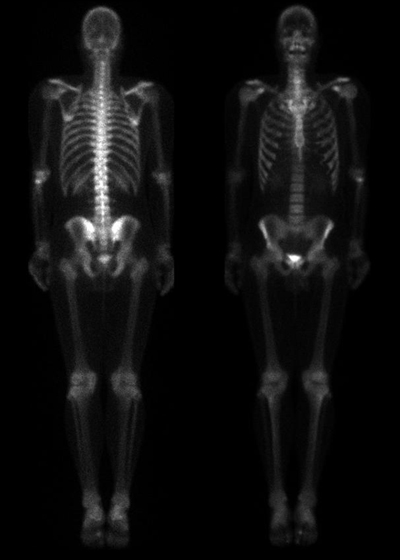
\includegraphics[width=5.5cm]{nuclearMedicineBoneScan} % https://www.hey.nhs.uk/nuclearmedicine/scanners-cameras-and-images/
\end{flushright}


\section{Acquisition}
\begin{itemize}
\item \gls{PNI} is a medical imaging technique that
  creates two-dimensional (2D) projection images of the
  three-dimensional (3D) distribution of radioactive materials within
  a patient \cite{bushberg2011essential}.
\item A radioactive isotope, incorporated into a chemical substance
  called a radiopharmaceutical, is administered to the patient
  (orally, by injection, or inhalation).
\item Once distributed according to the patient's physiological
  status, these radioisotopes \popup{emit}{For example, Technetium-99m
    (Tc-99m) emits 140-keV gamma rays, which are commonly imaged.}
  gamma rays, X-rays, or \popup{annihilation photons}{An annihilation
    photon is a type of high-energy photon produced during a unique
    interaction called annihilation, where a positron (a positively
    charged electron) combines with an electron.}.
\item Since X-rays and gamma rays are emitted isotropically (equally
  in all directions) from the radionuclide within the patient,
  \popup{collimators}{In general, an Anger scintillation camera is
    used for this.} are necessary to define the trajectory of photons
  reaching the detector and create a projection image.
\end{itemize}

\section{Clinical applications}
\begin{itemize}
\item PNI is used for functional imaging, providing insight into the
  physiological conditions (such as hyperthyroidism
  \cite{abdulla2025molecular_imaging}) rather than just the anatomy
  \cite{bushberg2011essential}.
\item Images can reveal ``hot spots'' (areas of increased
  radiopharmaceutical concentration, e.g., stress fractures or
  metastases) or ``cold spots'' (areas where normal concentration is
  altered, e.g., \popup{perfusion defects}{A perfusion defect refers
    to an area within an organ or tissue where the normal blood flow
    or distribution of a diagnostic agent is impaired or reduced. In
    medical imaging, particularly nuclear medicine, it indicates a
    functional or physiological abnormality, such as infarction
    (tissue death due to lack of blood supply) or ischemia (reduced
    blood flow), rather than a purely anatomical one.}).
\end{itemize}
\vspace{-4ex}
\begin{figure}[!b]
  \centering
  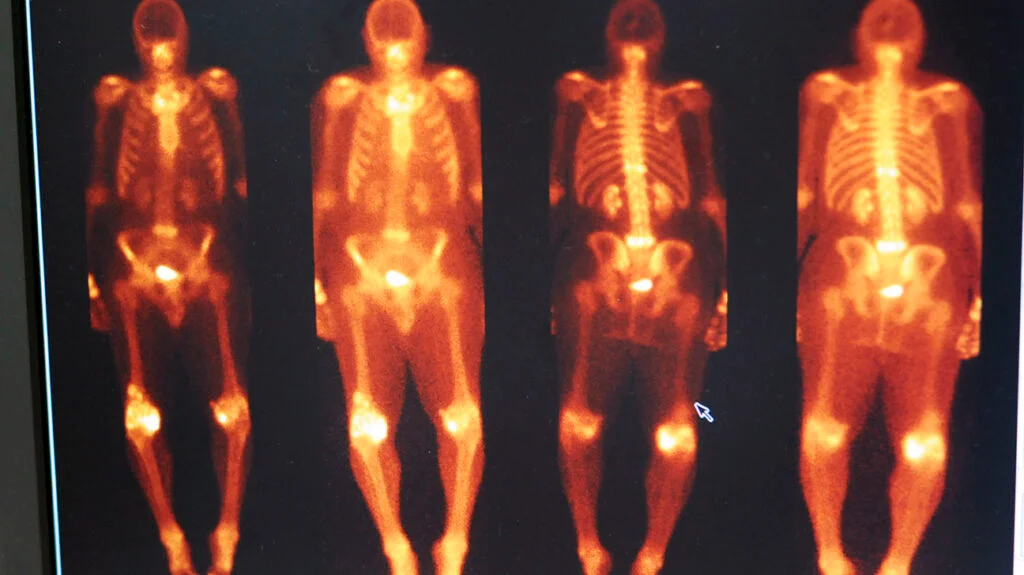
\includegraphics[width=6.5cm]{cardiac_amyloidosis}
  \caption{Hot spots showing the effects of \popup{Cardiac
      amyloidosis}{Amyloidosis occurs when the body produces amyloid
      proteins. Unlike other proteins, amyloid does not have a
      supportive role in the body. Instead, the buildup of amyloid
      protein leads to organ damage. Cardiac amyloidosis (CA) causes
      the heart to thicken and become inflexible due to abnormal
      deposits of protein in place of healthy heart tissue.}
    \cite{MNT_effects_cardiac_amyloidosis}.\label{fig:hot_spots}}
\end{figure}

\section{Quantum mottle}
\begin{itemize}
\item Due to patient safety reasons and the \popup{statistical
    nature}{Usually modeled by a Poisson distribution.} of the
  acquisition process, PNI usually generates images with a grainy
  appearance because the number of photons detected is, in most cases,
  very small.
\end{itemize}
\vspace{-4ex}
\begin{figure}[!b]
  \centering
  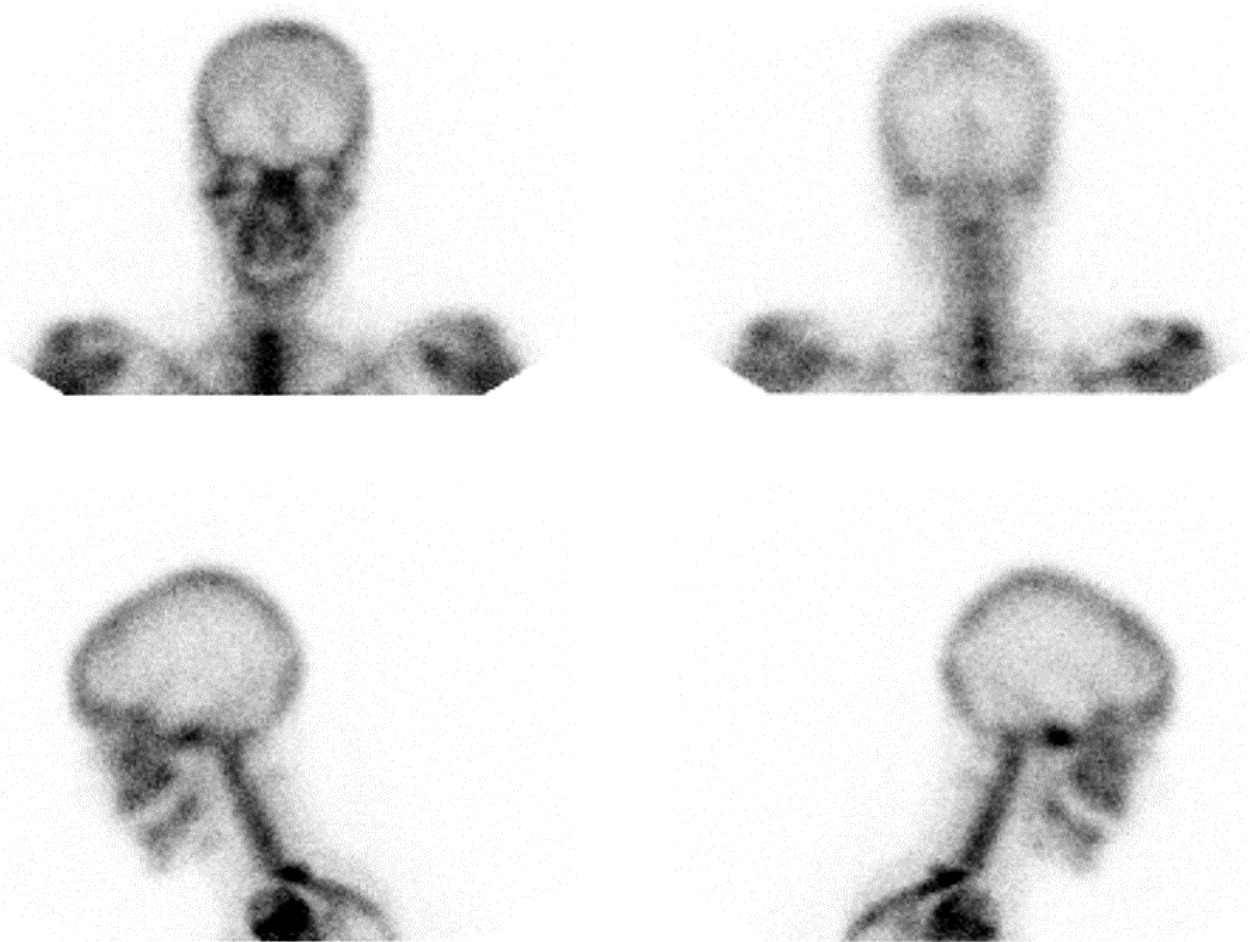
\includegraphics[width=6.5cm]{PNI_noise}
  \caption{Examples of quantum noise in \gls{PNI}.
    \cite{saridin2007quantitative}.}
  \label{PNI_noise}
\end{figure}

\section{Motion blur}
\begin{itemize}
\item As a consequence of images are acquired over \popup{many seconds
    or minutes}{Basically, to gain SNR.}, it is frequent to obtain
  moved images generated by \popup{patient motion}{For example,
    respiratory motion can not be avoided.}.
\end{itemize}
\vspace{-4ex}
\begin{figure}[!b]
  \centering
  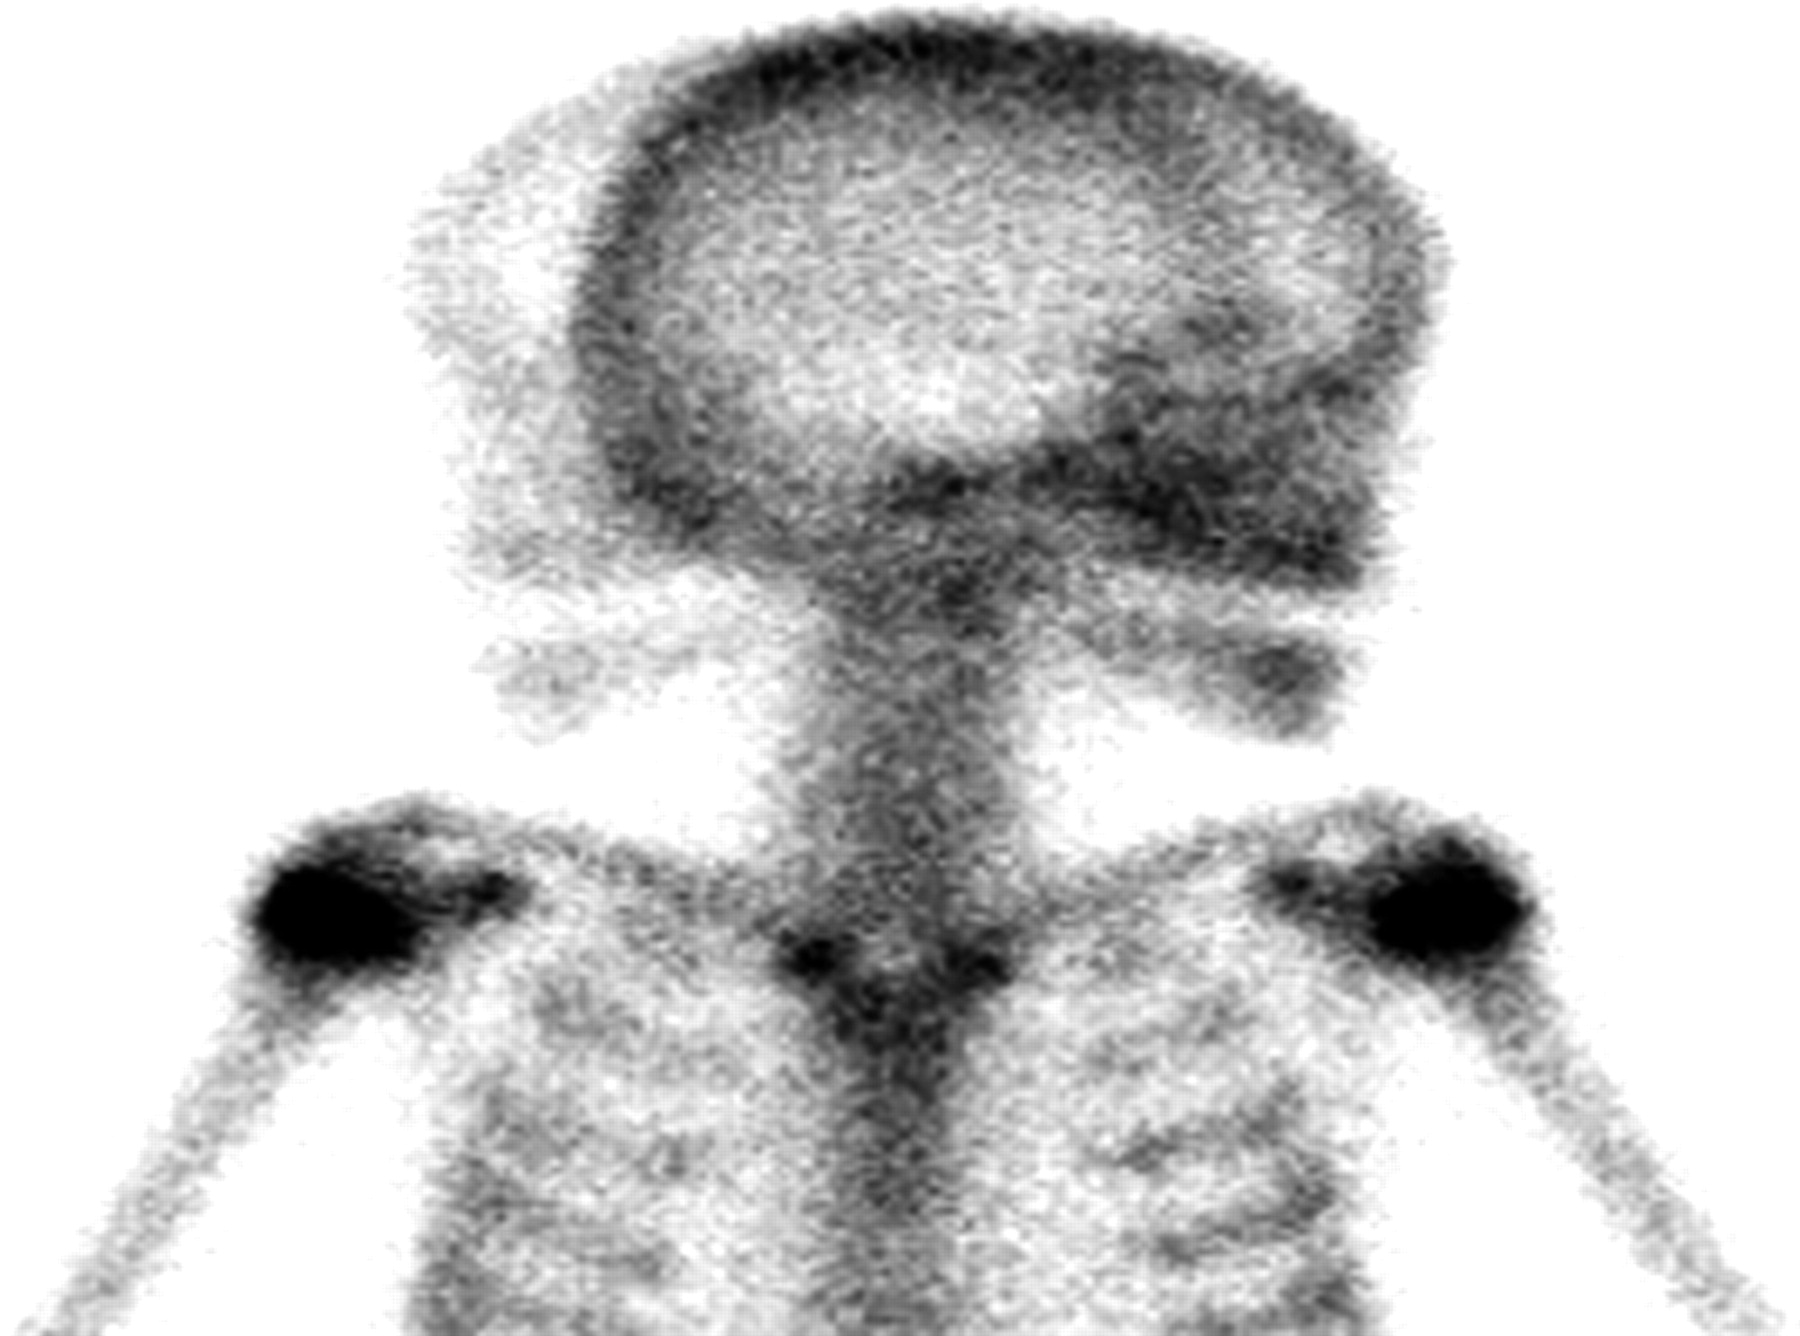
\includegraphics[width=6.5cm]{PNI_motion}
  \caption{Example of motion blur in \gls{PNI}.
    \cite{naddaf2004technical}.}
  \label{PNI_motion}
\end{figure}

%\chapter[\glsentrylong{SPECT} (\glsentryshort{SPECT})]{Single Photon Emission\\Computed Tomography (SPECT)}
\vspace{-45ex}
\begin{flushright}
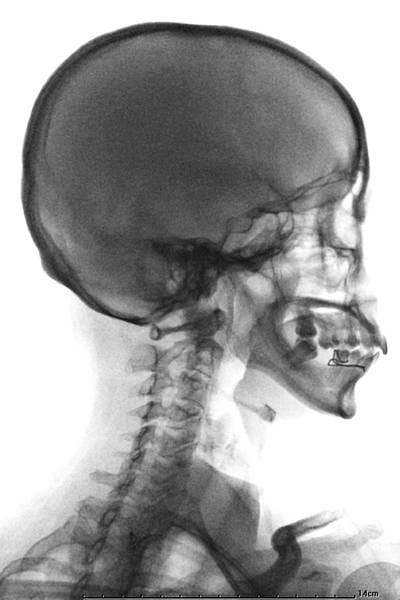
\includegraphics[width=4.5cm]{SPECT_example} % https://www.cidrad.com/wp-content/uploads/2024/06/testicular-ultrasound-riverside-county-ca-usa-near-me-400-600.jpg
\end{flushright}

\section{Acquisition}
\begin{itemize}
\item \gls{SPECT} is the tomographic counterpart of nuclear medicine
  planar imaging, just like CT is the tomographic counterpart of
  radiography \cite{bushberg2011essential,wikipedia_SPECT}.
  
\item In SPECT, a nuclear camera records X- or Gamma-ray emissions
  from the patient from a series of different angles around the
  patient.
  
\item  These projection data are used to reconstruct a series of
  tomographic emission images.

\item The spatial resolution of the images is inversely proportional
  to the distance between the patient and of the \popup{camera}{The
    camera uses a collimator to determine the direction of the
    photons. This generates a low detection efficiency because the
    collimator filters out over 99.9\% of the emitted photons. The
    design of the collimator inherently compromises between spatial
    resolution and detection efficiency}.
\end{itemize}

\section{Clinical applications}
\begin{itemize}
\item SPECT images provide diagnostic functional information similar
  to nuclear planar examinations (functional information about organ
  physiology) ; however, their tomographic nature allows physicians to
  better understand the precise distribution of the radioactive agent,
  and to make a better assessment of the function of specific organs
  or tissues within the body.
\item The same radioactive isotopes are used in both planar nuclear
  imaging and SPECT \cite{bushberg2011essential}.
\end{itemize}

\section{Image quality}
\begin{itemize}
\item The resolution is limited (hundres of pixels in each dimension)
  by two reasons:
  \begin{enumerate}
  \item The detection efficiency (which is very low) depends on the
    pixel-size.
  \item Each projection requires dozens of seconds
    \cite{abdulla2025SPECT}.
  \end{enumerate}
\item Althought it is based on the same imaging technology than PNI,
  it usually provided improved contrast and reduced structural noise
  by averaging counts from overlapping structures
\end{itemize}
%\chapter[\glsentrylong{PET} (\glsentryshort{PET})]{Positron Emission\\Tomography (PET)}
\vspace{-40ex}
\begin{flushright}
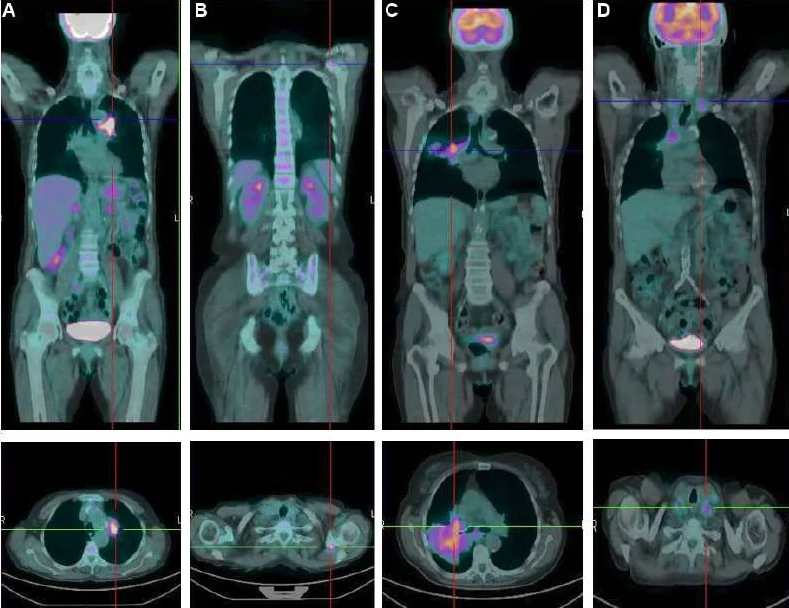
\includegraphics[width=6.5cm]{PET} % https://ksimg.com/wordpress/wp-content/uploads/2022/02/pet-ct.jpg
\end{flushright}

\section{Acquisition}
\begin{itemize}
\item Such as SPECT, PET is a tomographic nuclear imaging system
  \cite{abdulla2025PET,wikipedia_PET}.
\item Employs \popup{annihilation coincidence detection
    (ACD)}{Positron-emitting radioisotopes decay and release a
    positron. This positron travels a short distance, then annihilates
    with an electron from the surrounding tissue, converting their
    mass into two 511-keV photons. These two photons are emitted
    simultaneously and in nearly opposite directions (approximately
    180 degrees apart). PET scanners detect these coincident photon
    pairs using rings of detectors and specialised circuitry. ACD is
    significantly more efficient than collimation and avoids the
    degradation of spatial resolution with increasing distance from
    the detector.} instead of collimation to determine the procedence
  of the radiation that reach the detector.
\item Only uses \popup{positron-emitting radionuclides}{F-18
    fluorodeoxyglucose (FDG) is the most widely used PET
    radiopharmaceutical. Due to their generally short half-lives, PET
    radionuclides often require a cyclotron to be located nearby or
    on-site}.
\item PET scanners are more ``open'' than SPECT scanners because the
  resolution of the images is not so dependent on the distance of the
  camera to the patiend.
\item PET is \popup{more expensive}{A PET/CT system can cost
    approximately twice that of a SPECT/CT system} than SPECT.
\end{itemize}

\section{Clinical applications}
\begin{itemize}
\item As SPECT, it is mainly used to \popup{visualise physiological
    function}{The most common application of PET (especially with F-18
    FDG) is in oncology for differentiating malignant neoplasms,
    staging cancer, and monitoring treatment response.}
  \cite{bushberg2011essential}.
\end{itemize}

\section{Image quality}
\begin{itemize}
\item Compared to SPECT, PET has much higher count rate sensitivity
  and, generating less noise.
\item Therefore, PET images can be reconstructed with much higher
  spatial frequency \cite{abdulla2025NIQ}.
\end{itemize}

%\chapter{Magnetic Resonance Imaging (MRI)}

\section{Acquisition}
\gls{MRI}
\cite{westbrook2018mri,Wu2022MRI_Physics,thePIRL2018NMR_basics,thePIRL2018SpinEcho,thePIRL2018Fourier,thePIRL2018GRE}
is a technique (usually used in medicine) to obtain detailed views of
(usually living) samples (tissues, organs, and even a complete
organism). The sample is subjected to a magnetic field (in the order
of Teslas (T), called the B0 field) which is strong enough to align
the tiny magnetic fields generated by the hydrogen atoms (in reality,
the magnetic fields are a consequence of the magnetic activity of the
protons in the nuclei) that behave as small compasses. The scanner
(that basically is a tube) has also a tubular coil (forming another
concentric tube) to generate a gradient in the magnetic field which
encodes the 3D position of the hydrogen atoms.\footnote{The purpose of
  these gradients is to spatially encode the signal, allowing the MRI
  system to calculate how much signal is coming from each
  three-dimensional location (voxel) in the patient.}  Finally,
closest to the sample\footnote{The RF coil(s) is(are) typically placed
  as close to the anatomy under examination as possible to maximize
  signal reception.}, there is a third tubular concentric coil that
acts as a RF antenna, which emmit a signal to which the hydrogen atoms
are sensible\footnote{The RF excitation pulse (also known as B1
  field), which causes hydrogen nuclei to absorb energy and resonate
  if the pulse's frequency matches their Larmor frequency.}, and also
can receive the signal that the atoms emit when the RF signal
disapears (relaxation), until they recover their equilibrium state
(the alignment).\footnote{When the RF excitation pulse is switched
  off, the hydrogen nuclei lose the absorbed energy through a process
  called relaxation. This relaxation involves the recovery of
  longitudinal magnetization (the NMV (Net Magnetic Vector) realigns
  with B0) and the decay of coherent transverse magnetization.}

The signal received is an echo, which is a waveform representing
spatial frequencies from a selected slice (tomogram\footnote{A
  tomogram is an image that represents a slice or section of an 3D
  object,}). The contrast in this signal is determined by the
time-varying relaxation properties (T1 recovery and T2 decay) of the
tissues within that slice. This analog signal is digitized (converted
into binary numbers) via analog-to-digital conversion (ADC). These
digitized data points are then stored in a matrix called k-space. The
k-space data structure stores data about the frequency and phase
changes of magnetic moments over distance (spatial frequencies), i.e.,
each complex number of this matrix represents a Fourier
coefficient. In fact, the matrix if the Fourier transform of a 2D
image (a slice of the 3D MRI volume). Notice that each coefficients
``speaks'' about (the frecuencies and phases of) the complete
slice. Slice-selection is achieved by applying a slice-select gradient
simultaneously with an RF excitation pulse that has a specific center
frequency. The gradient creates a frequency slope, and only nuclei
whose precessional frequency matches the transmitted RF frequency (at
a specific location along the gradient) will resonate, thus defining
the slice \cite{westbrook2018mri}.

To reconstruct the 3D MRI volume we need to compute the inverse
Fourier transform of each slice, which is usually performed with the
inverse Fast Fourier Transform (FFT). The output of each transform is
a 2D image. The output 3D volume is the stack formed by all the 2D
images.

The signal received by the antenna is a 2D signal (with the
time-variying state of the relaxation of the hydrogen atoms of a slice
of the sample) that, when it is digitalized, generate a matrix of
complex numbers (the so called \emph{k-space}) with a magnitude and a
phase of the average oscillation (resonance) of the protons of the
hydrogen atoms in each small 3D cuve of the field of view (FOV) of
interest). These matrix represent the Fourier cofficients of a 2D
image (a slice), of the 3D MRI image. Modifiying the signal that
controls the gradient, we can select different FOVs (slices).

\section{Characteristics of the volumes}
\begin{enumerate}
\item \textbf{Signal-to-Noise Ratio (SNR)}: Defined as the ratio of
  the amplitude of signal received to the average amplitude of the
  background noise. In the case of MRI depends on the strength of the
  signal received by the antenna (precession of coherent
  magnetization), and the strength of noise signal (random frequencies
  existing in space and time, primarily from thermal motion of the
  molecules (in the patient) and background electrical noise of the
  electronics). The SNR increases with the \emph{strength of
    B0}\footnote{As the magnetic field strength increases, the Net
    Magnetic Vector (NMV) increases, leading to more available
    magnetization and consequently higher SNR. Doubling the field
    strength approximately doubles the SNR \cite{westbrook2018mri}.},
  the \emph{proton density}\footnote{Areas with a high concentration
    of MR-active protons (e.g., the pelvis) yield higher signal and
    thus higher SNR, whereas areas with low proton density (e.g., the
    lungs) result in lower signal and SNR \cite{westbrook2018mri}.},
  the \emph{coil(s) efficiency and distance to the
    sample}\footnote{Basically, the SNR is proportional to the inverse
    of the diameter of the tube. The power of the excitation RF
    signals is also proportional to the SNR.}, the \emph{signal
    scanning times}\footnote{Longer TR (Time-Repetition) allows for
    greater longitudinal magnetization recovery, making more signal
    available for conversion to transverse magnetization, which
    typically improves SNR. Shorter TE (Time-Echo) allows less
    coherent transverse magnetization to decay before the echo is
    collected, resulting in higher SNR \cite{westbrook2018mri}.}, the
  \emph{Number of Signal Averages (NSA)}\footnote{Increasing the NSA
    directly increases SNR, as correctly encoded signal is reinforced
    while random noise averages out \cite{westbrook2018mri}.}, and the
  \emph{size of the voxels}\footnote{Larger voxels contain more spins,
    which contribute to a higher signal and consequently increased SNR
    \cite{westbrook2018mri}.}.
\item \textbf{Spatial resolution}: Defined as the ability to
  distinguish between two points as separate and distinct, is
  typically in the range of a fraction of milimeters (for example, 0.5
  mm). This characteristic depends fundamentally on the \emph{minimal
    slice-thickness} provided by the internal coil, the
  \emph{resolution of the k-space}, and on the \emph{magnetic field
    strength (B0)} to provide a high enought SNR.\footnote{The SNR
    increases with B0 and the voxel size, so, to increase the
    resolution (decrease the voxel size) we must keep high enough the
    SNR by increasing B0. Otherwise, the noise can make it difficult
    to recognize the pathology}
\item \textbf{Contrast}: In general, the contrast in an viewed image
  depends on the range of intensities displayed, that should be as
  large as possible.\footnote{In Magnetic Resonance Imaging (MRI),
    image contrast refers to the differences in signal intensity
    between various anatomical features, between anatomy and
    pathology, or between different tissues. This differentiation is
    crucial for identifying anatomical structures and detecting
    abnormalities within the body \cite{westbrook2018mri}.} However, a
  high contrast does not neccesaryly implies more perceived quality,
  because the number of different intensities should be also high
  enough (usually, at least different 64 intensities should be
  avaiable). In the case of MRI data, and considering that the quality
  is a subjective matter, an increase in the contrast (and therefore,
  a higher perceived quality that can help to improve the diagnostic)
  can be obtanied if we use \emph{image weighting} (for example,
  T2-weighted volumes usually enhances pathologies), \emph{contrast agents}
  (e.g., gadolinium) can selectively shorten relaxation times,
  increasing the contrast between pathology and normal anatomy, among
  \emph{other MRI contrast-enhancing techniques} (magnetization
  transfer contrast, phase-contrast MR angiography, or the use of
  presaturation pulses) \cite{westbrook2018mri}.
\end{enumerate}

\section{Resources}

\bibliography{MRI}


\part{Storage of medical Images}
%\part{Medical Images Storage}

\chapter{Basic concepts}

\section{Storage media charactaristics}
\begin{enumerate}
\item \textbf{Capacity}: This is the total amount of data that a
  storage medium can hold. It's typically measured in \popup{B}{byte}s
  (8 \popup{bits, where a bit represents a logical state with one of
    two possible values.}), \popup{KB}{kilobyte}s
  ($1\text{KB} = 2^{10}\text{B}$), \popup{MB}{megabytes}s
  ($1\text{MB} = 2^{10}\text{KB}$), \popup{GB}{gigabyte}s
  ($1\text{GB} = 2^{10}\text{MB}$), \popup{TB}{terabyte}s
  ($1\text{TB} = 2^{10}\text{GB}$), and \popup{PB}{petabyte}s
  ($1\text{PB} = 2^{10}\text{GB}$).
\item \textbf{Volatility}: If the media need to connected to a current supply (for example, the \gls{RAM} memory of a computer), the media is said \emph{volatile}.
\item \textbf{\gls{WORM}}: A \gls{CDROM}, for example.
\end{enumerate}
\begin{itemize}
\item There are many storage media capable of storing digital images (some allow
\begin{enumerate}
\item 
\item Common massive storage systems (not only used for medical images) are:
\begin{enumerate}
\item \textbf{Cloud Storage} (Google Drive, Microsoft One Drive,
etc.): data is stored in remote servers accessed over the Internet.
\item \textbf{NAS (Network-Attached Storage)}: data is stored in a
\popup{specialized computer}{The computer rarely has a keyboard or
monitor, and has many hard drive bays.} (connected to the
\popup{LAN}{Local Area Network.}) that usually mounts several disks
with some type of \popup{RAID}{Redundant Array of Independent Disks.}
configuration.
\end{enumerate}
\end{itemize}
\vspace{-4ex}
\begin{figure}[!b]
  \centering
  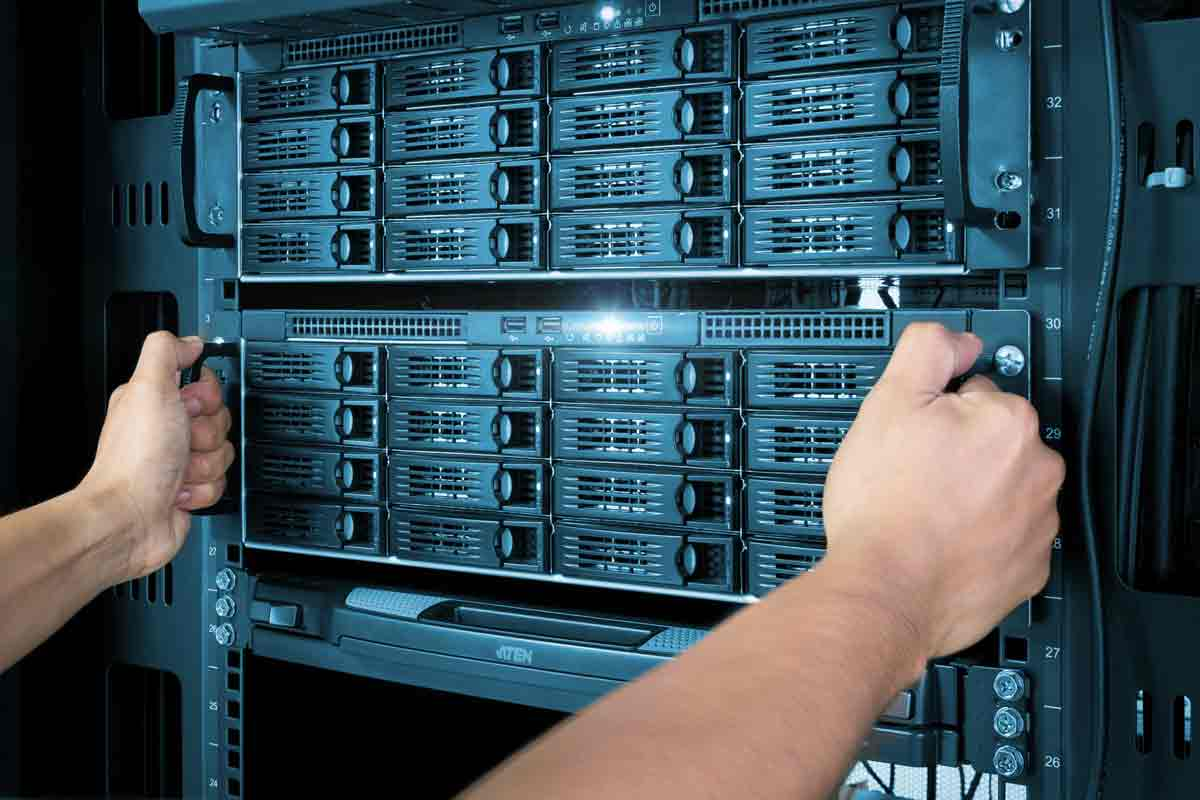
\includegraphics[height=3.5cm]{servidor-nas}
  \caption{A NAS \cite{AURUM_NAS}.\label{fig:NAS}}
\end{figure}

\section{Arrays of redundant disks}
\begin{itemize}
\item A \gls{RAID} is a logical disk that is able to work even when some of the \popup{physical disks}{That actually store the data.} fail. These are some of the existing configurations:
  \begin{enumerate}
  \item RAID-0 (Striping): \popup{No redundancy}{To maximize capacity,
      splits data across drives. This means that if a physical disk
      stops working, a loss of data will happen.}.
  \item RAID-1 (Mirroring): \popup{Maximum redundancy}{All physical
      disks contain the same data. To lost data all disks must fail at
      the same time.}.
  \item RAID-5 (Striping with Parity): \popup{One disk
      redundancy}{This configuration can only tolerate the failure of
      one disk.}. When the broken disk is replaced, the RAID must rebuild the parity information. During this time, no other disk can fail.
  \item RAID-6 (Double Parity): \popup{Two disks
      redundancy}{Tolerate the failure of
      two disks at the same time.}.
  \end{enumerate}
\end{itemize}

\section{Files and streams}
\begin{itemize}
\item A \popup{file}{Also known as ''archive''.} is a collection of data \popup{stored}{Files are
persistent: once written, they stay there until deleted.} on a storage
medium (for example, a NAS) with a defined structure and a
name. Example: a DICOM file.
\item A stream is a continuous flow of data that is transmitted and
processed in real-time, often without being stored
permanently. Example: a videcon between a patient and a doctor.
\item Files can be \popup{accesed randomly}{We can move over the file
to read or modify a part of it.}. Streams cannot (only are accesed
sequentially).
\end{itemize}

\section{Formats}
\begin{itemize}
\item Files and streams must follow some predefined structure and
encodings that indicate how to recover the information contained.
\item Most of the image formats used in medicine follow some standard
which define they, such as for example, the DICOM format.
\end{itemize}

\section{Data compression}
\begin{itemize}
\item Images requires large amounts of data to be represented. Data
compression define the objective of an efficient encoding system:
reduce the lendth of files and streams.
\item Data compressors can be:
\begin{enumerate}
\item \textbf{Lossless}: If after the decompression we recover all the
compressed information, to the point that the original file/stream can
be regenerated.
\item \textbf{Lossy}: when not. The advantage is that the compression
ratios are much higher, and sometimes the loss can be aceptable.
\end{enumerate}
\end{itemize}

\section{PACS (Picture Archiving and Communication System)}

The hospital system used to store, retrieve, and display medical images.

Replaces old physical films with digital archives.

Typically linked to the Electronic Health Record (EHR) so patient information and images are synchronized.

\section{long-term persistency, Data Sequrity and Privacy}
Patient images are protected health information (PHI).

Systems must follow laws like HIPAA (USA) or GDPR (Europe) for confidentiality.

Images should only be accessed by authorized healthcare professionals.
%\chapter{\glsentrylong{PNG}}

\section{\glsentrylong{W3C} international standard}
\begin{itemize}
\item Developed by the \href{https://www.w3.org/}{W3C}, \gls{PNG} \cite{roelofs1999png} is
  supported by all Web browsers, and most image viewers.
\end{itemize}
%\vspace{-4ex}
\begin{center}
  \href{https://upload.wikimedia.org/wikipedia/commons/0/05/CT_of_a_normal_abdomen_and_pelvis%2C_coronal_plane_79.png}{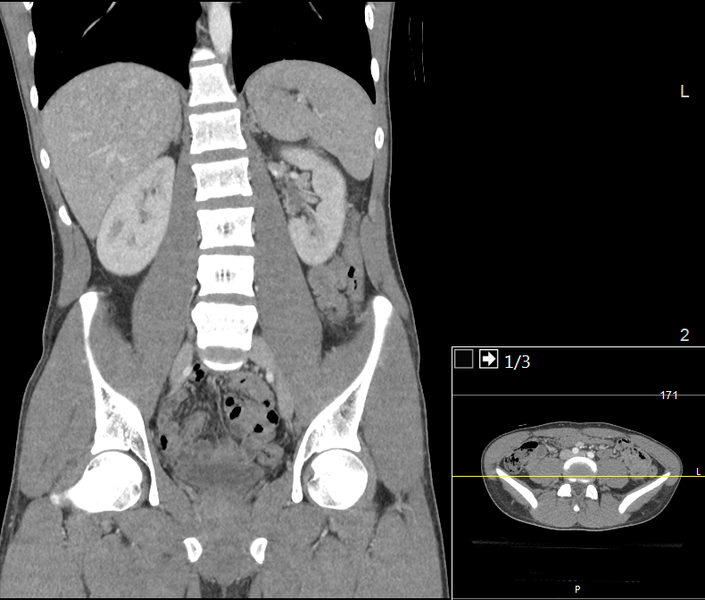
\includegraphics[width=6cm]{CT_example}}\\
     (click on the image)
\end{center}

\section{Raster graphics file format}
\begin{itemize}
\item Up to ($2^{32}-1$)x($2^{32}-1$) pixels, efficiently represented (lossless compression).
\item Pixels can be gray-scale (1 channel) or color
  \popup{\gls{RGBA}}{Red, Green, Blue, and Alpha (transparency)
    channels. The alpha-channel is optional.} (4 channels).
\end{itemize}
\vspace{-4ex}
\begin{center}
  \href{https://en.wikipedia.org/wiki/Raster_graphics}{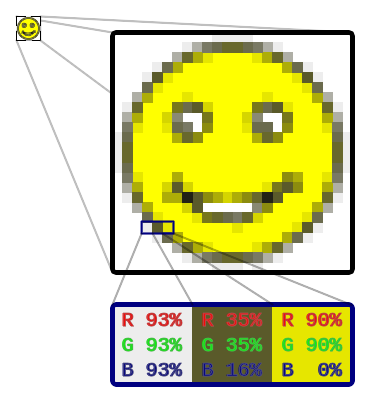
\includegraphics[width=5cm]{RGB-raster-image}}
\end{center}

\section{8 and 16 bits/channel}
\begin{itemize}
\item In gray-scale image:
  \begin{center}
    \begin{tabular}{c|c}
      & Number of \\
      Bits/channel & gray-scale values \\
      \hline
      8 & $2^8=256$ \\
      16 & $2^{16}=65536$
    \end{tabular}
  \end{center}
\item These pixel ``depth'' should be fine for most medical images.
\end{itemize}

\section{\popup{Animated}{Also called ``motion''.} PNG}
\begin{itemize}
\item A \gls{APNG} is sequence of images in a \gls{PNG} file.
\end{itemize}
\begin{center}
  \href{https://commons.wikimedia.org/wiki/Category:Animated_PNG_files#/media/File:201805_human_skeleton_anim.png}{\includegraphics[width=5cm]{human_skeleton_anim}} \\
  (Click in the image)
\end{center}

\section{Image metadata (1/2)}
\begin{itemize}
\item PNG images can store metadata:
  \begin{center}
    \begin{tabular}{l|l}
      Keyword & Explain\\
      \hline
      Title & Short (one line) title or caption for image \\
      Author & Name of image's creator \\
      Description & Description of image (possibly long) \\
      Copyright & Copyright notice \\
      Creation Time & Time of original image creation \\
      Software & Software used to create the image \\
      Disclaimer & Legal disclaimer \\
      Warning & Warning of nature of content \\
      Source & Device used to create the image \\
      Comment & Miscellaneous comment; conversion from GIF comment
    \end{tabular}
  \end{center}
\end{itemize}

\section*{Image metadata (2/2)}
\begin{itemize}
\item
  \href{https://github.com/vicente-gonzalez-ruiz/medical_imaging/blob/main/notebooks/PNG_add_metadata.ipynb}{Here}
  there is an example that shows and modifies the metadata in a PNG
  image.
\end{itemize}
%\chapter{\gls{JPEG}}

\section{\gls{ITU} standard}
\begin{itemize}
\item Supported by all Web browsers, and most image viewers, define
  how to compress raster images \cite{ccitt.t81}.
\item Developed by the \gls{JPEG} (\href{https://www.itu.int}{ITU}),
  in 1992.
\end{itemize}
\vspace{-2ex}
\begin{center}
  \href{https://en.wikipedia.org/wiki/Magnetic_resonance_imaging_of_the_brain#/media/File:MRI_of_Human_Brain.jpg}{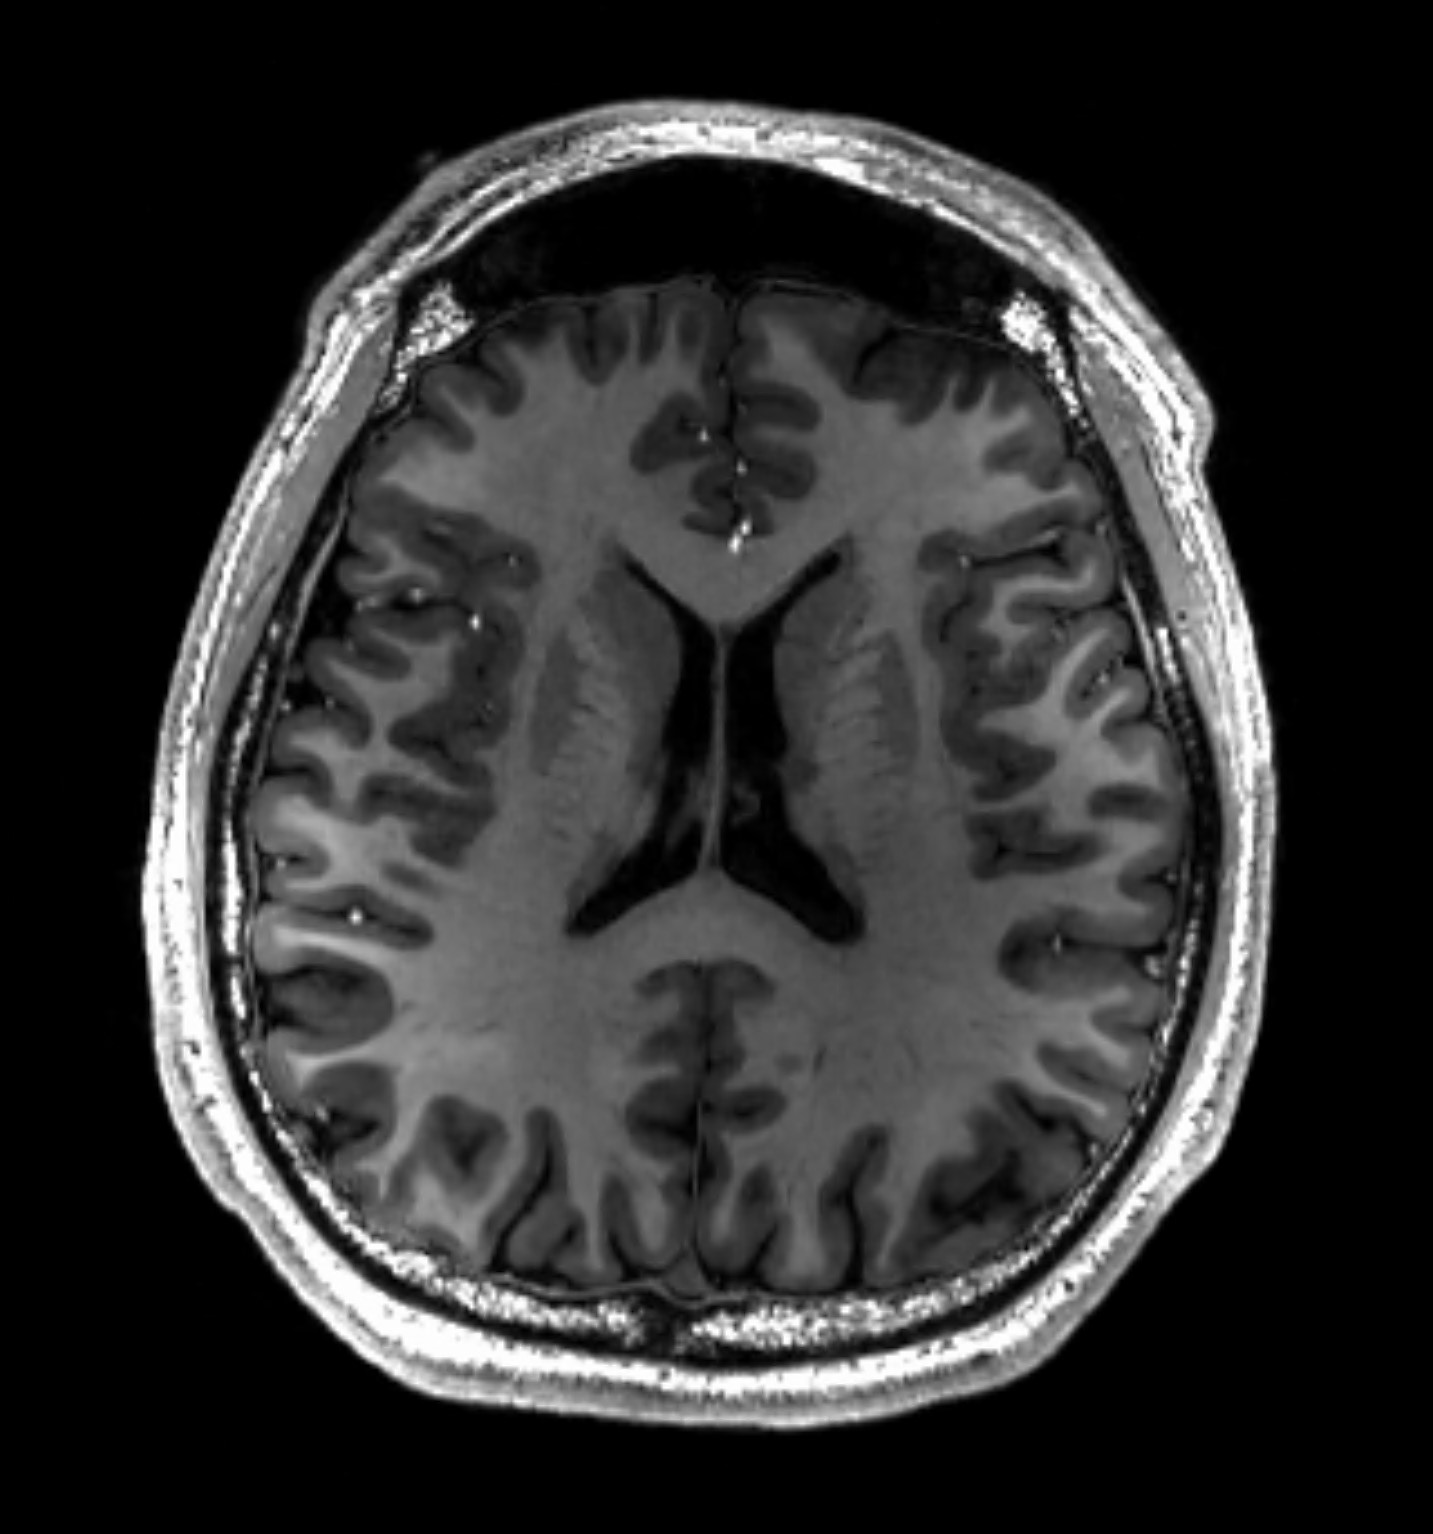
\includegraphics[width=4.0cm]{MRI_of_Human_Brain}}\\
  (click on the image)
\end{center}

\section{Lossy compression of color natural images}
\begin{itemize}
\item Designed for achieve high compression ratios, but at the expense of reducing quality.
  \item Raster images with up to ($2^{16}-1$)x($2^{16}-1$) pixels.
  \item Pixels must be gray-scale or \gls{RGB}, 8 bits/channel.
\end{itemize}
\vspace{-2ex}
\begin{center}
  \href{https://www.thewebmaster.com/jpeg-definitive-guide/}{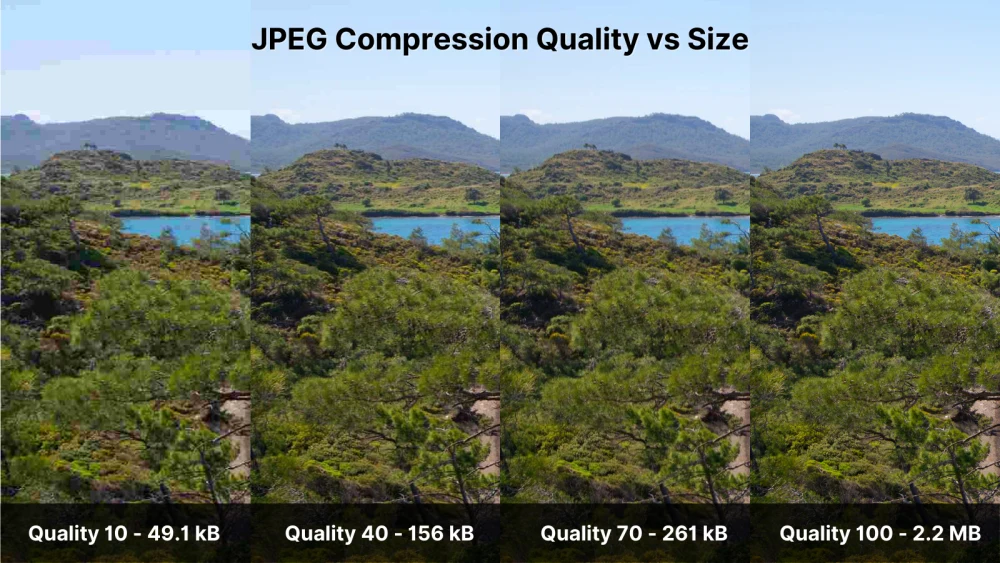
\includegraphics[width=8.5cm]{JPEG_Quality_vs_Size}}
\end{center}

\section{Algorithm}
\begin{enumerate}
\item Convert from the \gls{RGB} color space to the \gls{YCbCr} color
  space. Only if the input image is in color.
\item Subsample the crominance (Cr and Cb channels). /* Lossy step */
\item Divide each channel in blocks of size 8x8. \popup{The rest of
    steps work by blocks}{This makes it possible to work at the block
    level regardless of the image size.}.
\item Transform each block using the \gls{DCT}.
\item Quantize the \gls{DCT} coefficients. /* Lossy step */
\item Entropy encode the quantized coefficients.
\end{enumerate}

\section*{}
\begin{itemize}
\item A graphic description of a compression of a gray-scale image.
\end{itemize}
\vspace{-2ex}
\begin{center}
  \href{https://link.springer.com/article/10.1007/s40799-019-00358-4}{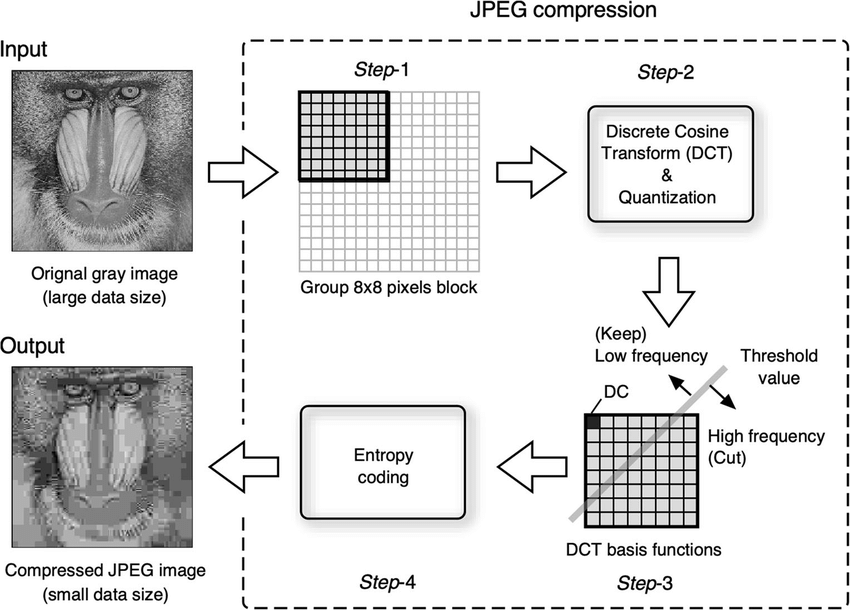
\includegraphics[width=8.5cm]{JPEG}}
\end{center}

\section{Artifacts}
\begin{itemize}
\item The human eye is sensitive to the 8x8-blockiness.
\end{itemize}
\vspace{-2ex}
\begin{center}
  \href{https://thesai.org/Publications/ViewPaper?Volume=6&Issue=4&Code=ijacsa&SerialNo=16}{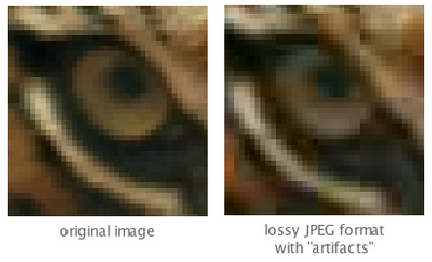
\includegraphics[width=10cm]{JPEG_blocking}}
\end{center}

\section{Progressive rendering}
\begin{itemize}
\item Optinal. Blocks are reconstructed coefficient-by-coefficient following the Zig-Zag ordering.
\item During a progressive visualization, blocks display higher
  spatial frequencies.
\end{itemize}
\begin{center}
  \href{https://es.m.wikipedia.org/wiki/Archivo:Zigzag_scanning.jpg}{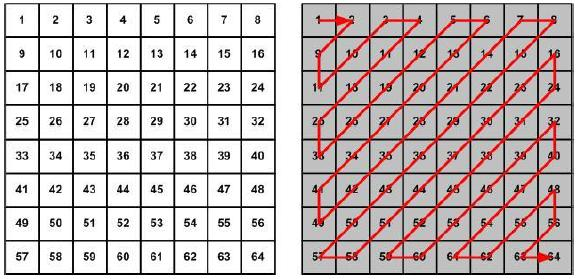
\includegraphics[width=8cm]{Zigzag_scanning}}
\end{center}

\section{Metadata}
\begin{itemize}
\item \gls{JPEG} images can store metadata as
  \href{https://en.wikipedia.org/wiki/Exif}{Exif} data (see the \href{https://gitlab.com/TNThieding/exif/-/blob/master/docs/api_reference.rst?ref_type=heads}{Exif implementation}). Some fields are:
  \vspace{-2ex}
  \begin{center}
    \begin{tabular}{l|l}
      Keyword & Meaning\\
      \hline
      ImageWidth & Width of the image in pixels \\
      ImageLength & Height of the image in pixels \\
      BitsPerSample&  Number of bits per color \\
      Make & Manufacturer of the camera or scanner \\
      Model & Model of the camera or scanner \\
      Software & Software used to process the image \\
      Orientation & Of the camera when the image was taken \\
      DateTimeOriginal & Date and time the image was originally captured \\
      ExposureTime & hutter speed \\
      FNumber & Lens aperture setting \\
      FocalLength & Focal length of the lens \\
      UserComment & User's comments about the image
    \end{tabular}
  \end{center}
\end{itemize}

\section*{}
\begin{itemize}
\item
  \href{https://github.com/vicente-gonzalez-ruiz/medical_imaging/blob/main/notebooks/JPEG_add_metadata.ipynb}{Here}
  there is an example that shows and modifies the metadata in a JPEG
  image.
\end{itemize}

%\chapter{JPEG2000}
\label{cha:JPEG2000}

\section{\acrshort{ISO} international standard}
\begin{itemize}
\item Developed by the \gls{JPEG} (ISO/IEC 15444\href{https://www.itu.int}{ITU}),
  the JPEG2000 standard \cite{taubman2002jpeg2000} in 2000, as a successor of
  \gls{JPEG}.
\item Mainly used in medical imaging and digital cinema.
\end{itemize}
\vspace{-2ex}
\begin{center}
  \href{https://en.wikipedia.org/wiki/Magnetic_resonance_imaging_of_the_brain#/media/File:MRI_of_Human_Brain.jpg}{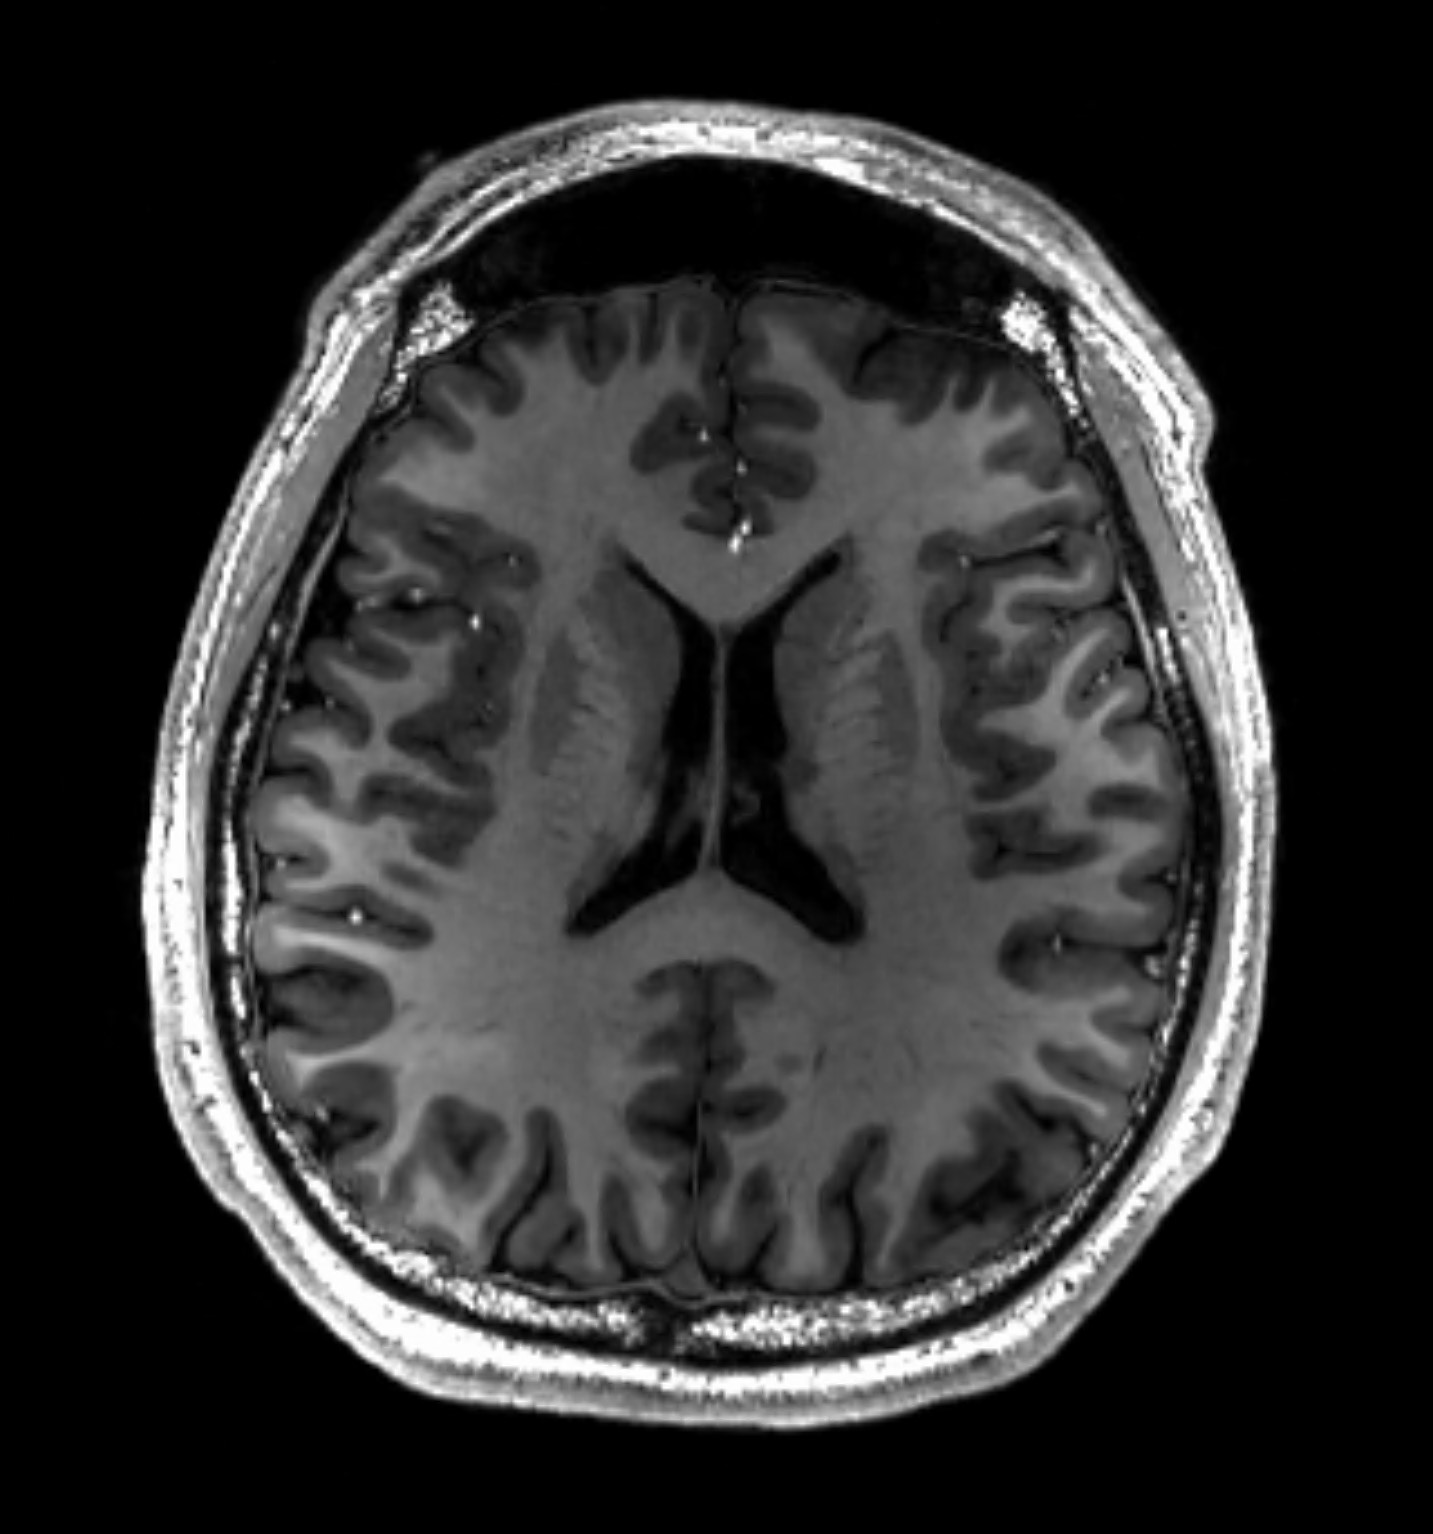
\includegraphics[width=4.0cm]{MRI_of_Human_Brain}}\\
  (click on the image)
\end{center}

\section{Lossless and lossy compression}
\begin{itemize}
\item Two different compression modes:
\item \textbf{Reversible}: Allows a perfect reconstruction of the raster image (like \gls{PNG}).
\item \textbf{Irreversible}: Unable to recover all the visual
  information, but offers a better rate/distortion performance than
  the reversible mode for the same bit-rate.
\end{itemize}

\section{16-bit per channel and several color spaces support}
\begin{itemize}
\item \popup{16 bits/pixel offers enough quality for specialized
    applications such as medicine, atronomy, etc.}{It is quite
    difficult to increase the SNR above of 16 bits because basically
    we register noise when the amplitude of signal is small.}.
\item Apart from gray-scale and \gls{RGB}, JPEG2000 supports
  \gls{YCbCr}, \gls{sRGB} \cite{sRGB_wikipedia}, \gls{CIELAB}
  \cite{CIELAB_wikipedia}, and \popup{custom}{It is posible to define
    a color transform.} \cite{houchin2001specification} color spaces.
\end{itemize}

\section{Superior compression efficiency than \gls{JPEG}}
\begin{itemize}
\item Better quality at the same bitrate compared to JPEG \cite{vruiz_J2K}.
\end{itemize}
\begin{center}
  \begin{tabular}{cc}
    \multicolumn{2}{c}{Lena at 0.1 bits/pixel} \\
    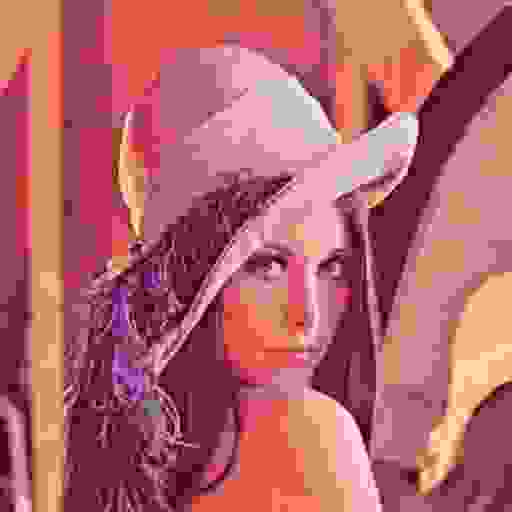
\includegraphics[width=5cm]{lena_01} & 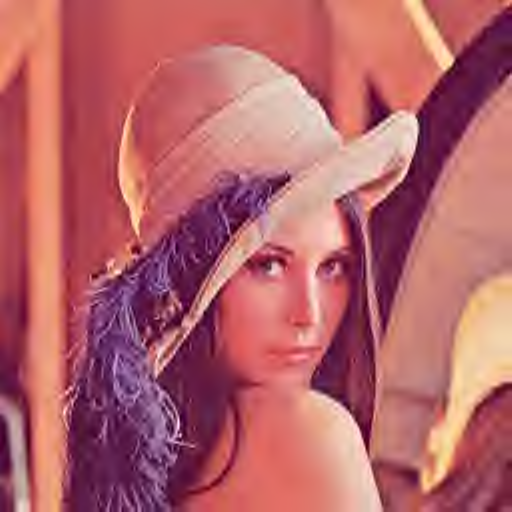
\includegraphics[width=5cm]{lena_01_jp2} \\
    JPEG & JPEG2000
  \end{tabular}
\end{center}

\section{Baseline algorithm (1/2)}
\begin{enumerate}
\item Convert from the \gls{RGB} color space to the \gls{YCbCr} color
  space. Only if the input image is in color and not in \gls{YCbCr}.
\item Transform each \gls{YCbCr} component using the 2D-\gls{DWT}.
\item If we are using the irreversible mode, quantize the \gls{DWT}
  coefficients. /* Lossy step */
\item Entropy encode the quantized coefficients with \gls{EBCOT}.
\end{enumerate}

\section{Structure of an image in the DWT domain}
\begin{itemize}
\item The \gls{DWT} represents signals as a multiresolution structure
  \cite{vruiz_J2K}.
\end{itemize}
\vspace{-2ex}
\begin{center}
  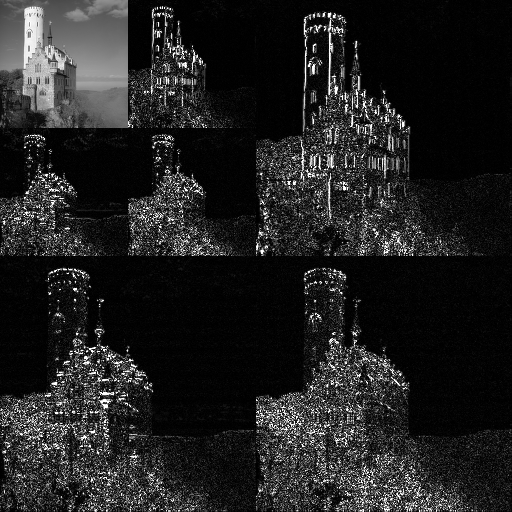
\includegraphics[width=6cm]{2-level_wavelet_transform-lichtenstein}
\end{center}

\section{Spatial scalability}
\begin{itemize}
\item When the image is rendered by resolution levels.
\end{itemize}
\vspace{-2ex}
\begin{center}
  \resizebox{11cm}{!}{
    \begin{tabular}{ccc}
      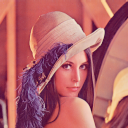
\includegraphics{lena_128x128_rgb} & 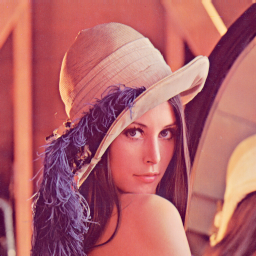
\includegraphics{lena_256x256_rgb} & 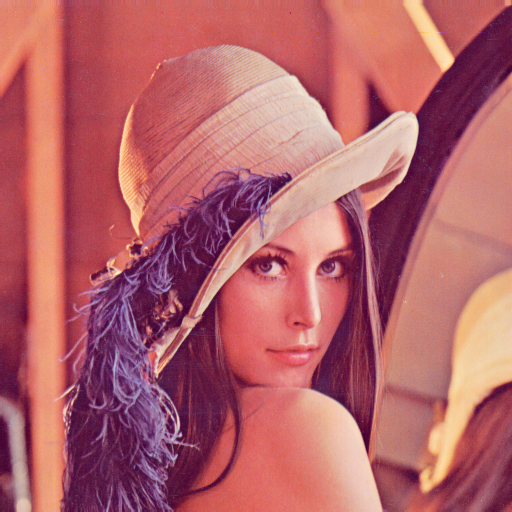
\includegraphics{lena_512x512_rgb}
    \end{tabular}
  }
\end{center}

\section{Quality scalability}
\begin{itemize}
\item When the image is rendered by \popup{coefficient amplitude}{DWT
    coefficients are actually decoded based on their contribution to
    the rate/distortion (R/D) curve. An R/D curve relates (X-axis) the
    amount of decompressed data versus (Y-axis) the achieved
    distortion. Depending on the distortion metric used, the curve may
    decrease with increasing number of decompressed bits (e.g., when
    measuring MSE) or increase with increasing number of decompressed
    bits (e.g., when measuring SNR).} \cite{vruiz_J2K}.
\end{itemize}
\vspace{-2ex}
\begin{center}
  \begin{tabular}{ccc}
    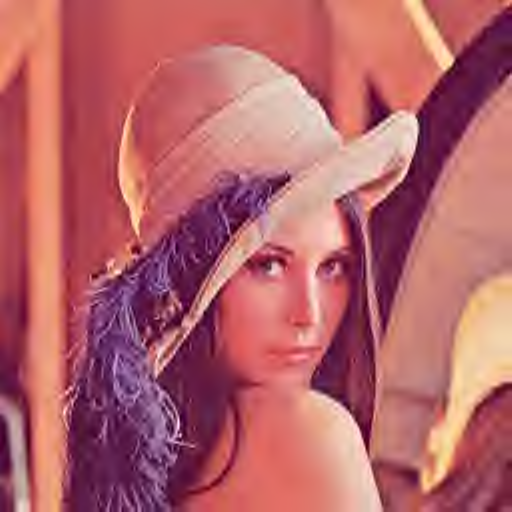
\includegraphics[width=4.0cm]{lena_01_jp2} & 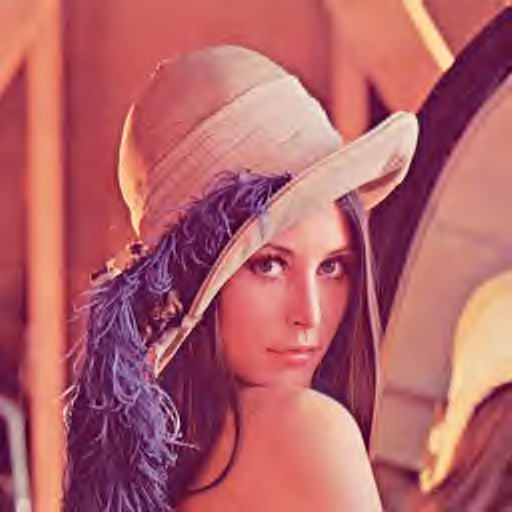
\includegraphics[width=4.0cm]{lena_02_jp2} & 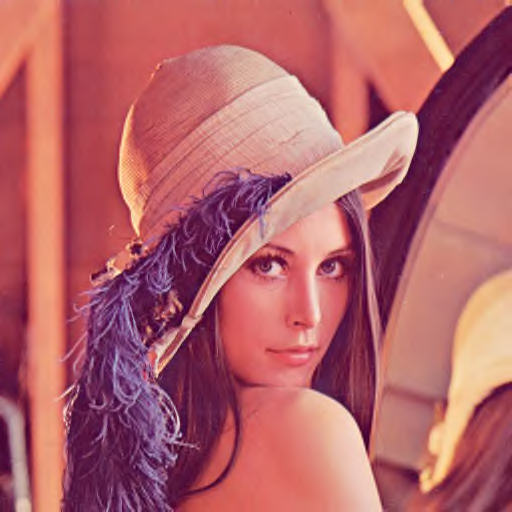
\includegraphics[width=4.0cm]{lena_05_jp2} \\
    0.1 bits/pixel & 0.2 bits/pixel & 0.5 bits/pixel
  \end{tabular}
\end{center}

\section{\acrshort{ROI} scalability}
\begin{itemize}
\item It is possible to dedicate more bit-rate to a \gls{ROI}, that
  can be defined interactively \cite{vruiz_J2K}.
\end{itemize}
\vspace{-2ex}
\begin{center}
   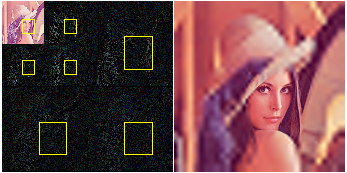
\includegraphics[width=11cm]{ROI}
\end{center}
  
\section{Error resilience}
\begin{itemize}
\item An error in JPEG 2000 tends to affect only localized image areas
  rather than corrupting the entire picture, due to the entropy coding
  of data in relatively small independent blocks
  \cite{wikipedia_J2K,brahimi2021efficient}.
\end{itemize}
\vspace{-2ex}
\begin{center}
  \href{https://flylib.com/books/en/2.537.1.37/1}{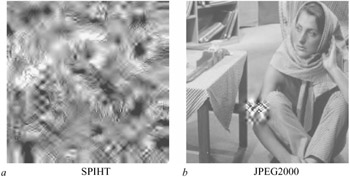
\includegraphics[width=11cm]{J2K_error_resilience}}
\end{center}

\section{3D support}
\begin{itemize}
\item Based on the 3D-DWT \cite{Bruylants_J2K_3D}.
\end{itemize}
\vspace{-2ex}
\begin{center}
  \href{https://spie.org/images/Graphics/Newsroom/Imported/0779/0779_fig1.jpg}{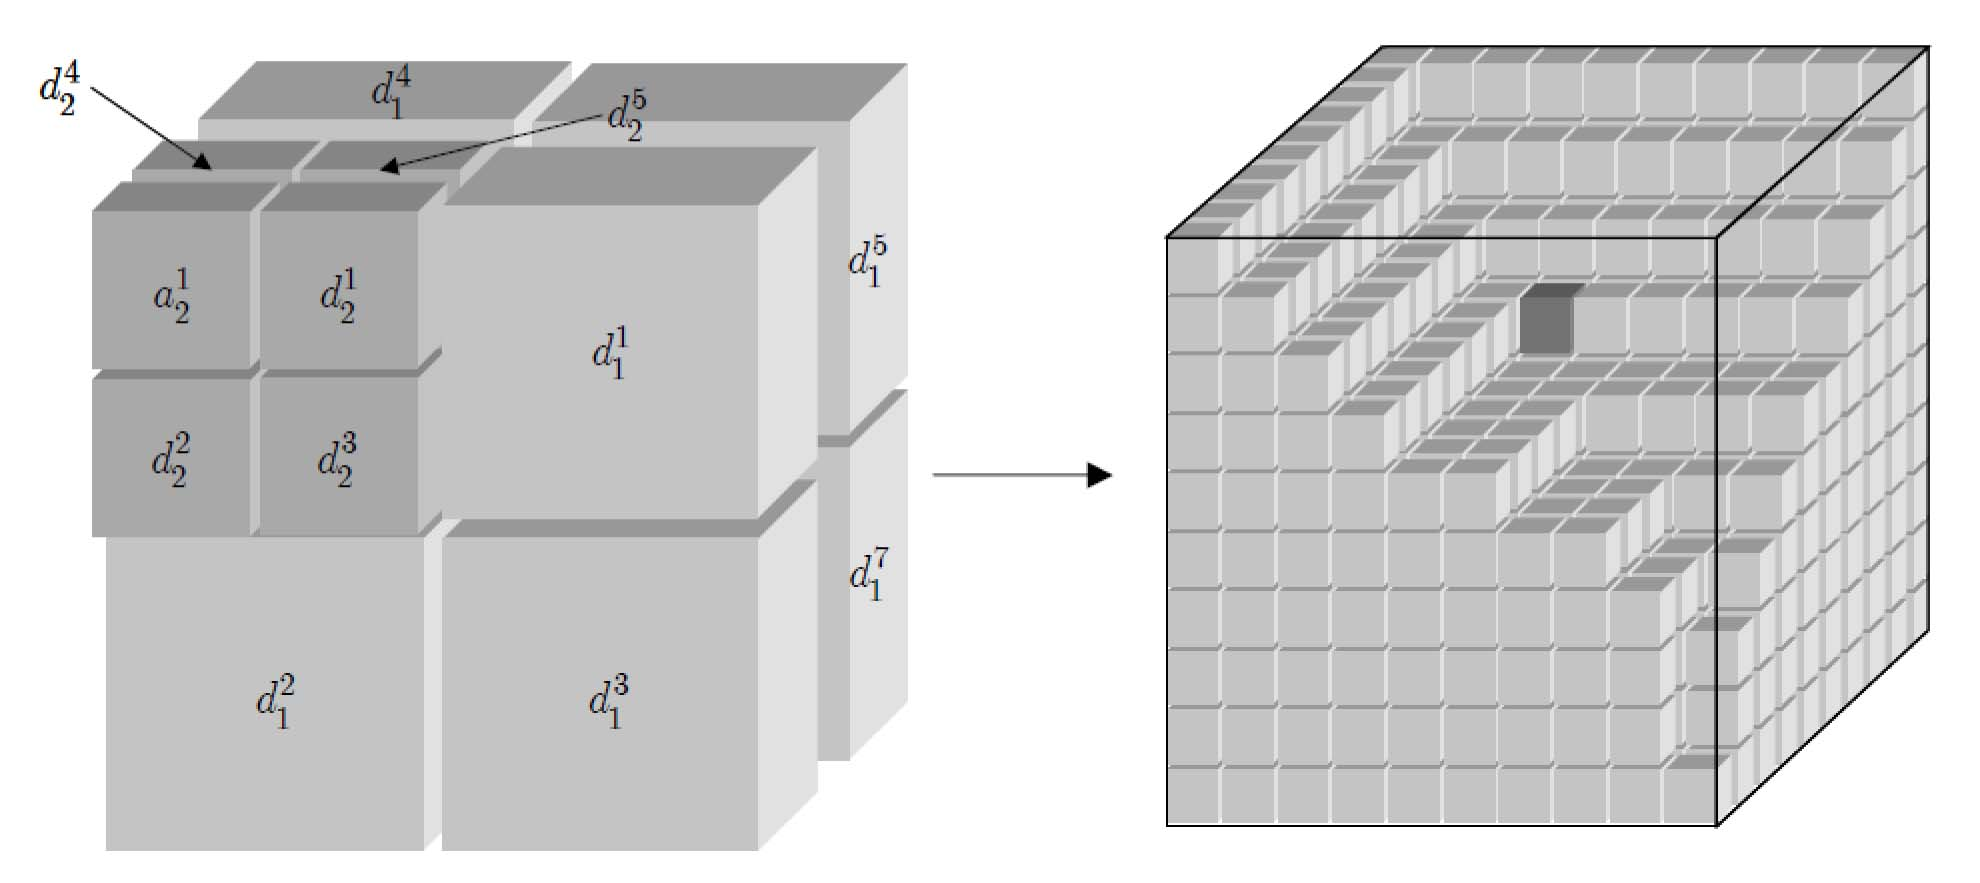
\includegraphics[width=11cm]{J2K_3D}}
\end{center}

\section{Motion JPEG2000 (digital cinema)}
\begin{itemize}
\item The movies played in digital cinemas leverage the spatial
  scalability provided by JPEG2000 to distribute a single DCP file
  that can be played in different resolution-capability beamers
  \cite{wikipedia_DCP}.
\item Each piture of the movie is compressed independently
  \cite{DigitalCinema}.
\end{itemize}
\begin{center}
  \href{https://vicente-gonzalez-ruiz.github.io/JPEG2000/}{\includegraphics[width=8cm]{MJ2K}}
\end{center}

\section{\gls{JPIP}}
\begin{itemize}
\item Based on the client/server model.
\item The client (the image viewer), \popup{interactively}{Usually
    controlled by a human.}, request to the server (that access to the
  JPEG2000 file \popup{locally}{Usually on a local disk.}) a sequence
  of \popup{\glspl{ROI}}{Actually, the term that the standard uses is
    ``WOI (Window Of Interest)''} \cite{ORTIZ04b}.
\item The server sends only those \popup{pieces of
    code-stream}{Data-bins} that are related with the current
  \gls{ROI} (which can be modified at any time). If the image is very
  big compared to the \gls{ROI}, this can save a lot of
  \popup{bandwidth}{In computer networks, bandwidth is a synonym of
    transmission capacity of the communication channel.}.
\end{itemize}
\begin{center}
  \href{http://www.hpca.ual.es/~vruiz/papers/ORTIZ04c.pdf}{\includegraphics[width=10cm]{JPIP}}
\end{center}

\section*{\gls{JPIP} example}
\begin{center}
  \href{https://ieeexplore.ieee.org/document/7214293}{\includegraphics[width=\textwidth]{JPIP_example}}
\end{center}

\section{Metadata}
\begin{itemize}
\item
  \href{https://github.com/vicente-gonzalez-ruiz/medical_imaging/blob/main/notebooks/JPEG2000_add_metadata.ipynb}{Here}
  there is an example that shows and modifies the metadata in a JPEG2000
  image.
\end{itemize}

%\chapter{\glsentrylong{MPEG} (\glsentryshort{MPEG})}
\label{cha:MPEG}

\section{A collection of standards}
\begin{itemize}
\item Developed by the \gls{MPEG} (\href{https://www.itu.int}{ITU}),
  in 1992  \cite{wikipedia_MPEG}.
\item Define different algorithms to compress sequences of raster
  images (videos) and the corresponding audio.
\item All are lossy encoders.
\end{itemize}

\section{Versions}
\begin{enumerate}
\item \href{https://en.wikipedia.org/wiki/MPEG-1}{\textbf{MPEG-1}}
  (1993): Designed to store a movie in a \gls{CD} (\gls{VCD}).
\item \href{https://en.wikipedia.org/wiki/MPEG-2}{\textbf{MPEG-2}}
  (1996): Used in \glspl{DVD}, \href{https://en.wikipedia.org/wiki/Satellite_television}{satellite TV} and \href{https://en.wikipedia.org/wiki/Digital_television}{terrestial TV} (\gls{DVB}).
\item \href{https://en.wikipedia.org/wiki/MPEG-4}{\textbf{MPEG-4}}
  (1998): Used mainly in media streaming on the Internet.
\end{enumerate}

\section{Algorithm}
\label{sec:MPEG-1_algo}
\begin{enumerate}
\item Convert to the \gls{YCbCr} color space, and
  \href{https://en.wikipedia.org/wiki/Chroma_subsampling}{subsample to
    4:2:0} (if the input is not yet in this format). /* Lossy */
\item Divide each channel in macro-blocks (MCs) of size 16x16. \popup{The
    rest of steps work by MCs}{This makes it possible to work
    at the MC level regardless of the image size.}.
\item \popup{Performing \gls{RDO}}{RDO implies that the video codec
    selects the optimal encoding decissions from a rate/distortion
    perspective. For example, if for the same quality (or distortion)
    a MB requires less bits if it is not motion compensated, then the
    codec does not compensate it. Thus, some MBs can be compensated
    while others not.},
  \href{https://en.wikipedia.org/wiki/Motion_compensation#Block_motion_compensation}{compensate
    the motion of each MC} using MCs of the \popup{adjacent
    images}{The MCs of the frame N, are compensated using the MCs of
    the frames N-1 and N+1.}. This step generates
  \popup{residue}{Residue MCs follow a Laplace distribution with mean
    0, and its entropy is smaller than the original MCs (this means
    that a residue MCs is more compressible than an original MC, on
    average).} MCs and a motion vector per MC, at
  \href{https://en.wikipedia.org/wiki/Motion_compensation}{half-\gls{PEL}
    accuracy}.
\item Divide each MC in $8\times 8$ blocks.
\item Transform each block using the \gls{DCT}.
\item Quantize the \gls{DCT} coefficients. /* Lossy */
\item \popup{Entropy encode}{Using a combination of RLE and Huffman
    coding.} the quantized coefficients and the motion compensation
  data (motion vectors and reference frames).
\end{enumerate}

\begin{figure}[H]
  \vspace{-2ex}
  \centering
  \href{https://w3.ual.es/~vruiz/Docencia/Apuntes/Coding/Video/02-MPEG1/index.html}{\includegraphics[height=\textheight]{MPEG-1_compressor}}
  \caption{The \gls{MPEG} compressor.}
  \label{fig:MPEG_compressor}
\end{figure}

\section{Blocking effect}
\begin{figure}[H]
  \vspace{-0ex}
  \centering
  \href{https://filmora.wondershare.com/video-editing/video-compression-artifacts.html}{\includegraphics[height=0.8\textheight]{MPEG_artifacts}}
  \caption{\gls{MPEG} compression artifacts.}
  \label{fig:MPEG_artifacts}
\end{figure}

%\chapter{\glsentrylong{AVC} (H.264)}

\section{Basics}
\begin{itemize}
\item Lossy and \popup{lossless}{Although by a large margin, it is
    mainly used as a lossy video codec.} \cite{wikipedia_AVC}.
\item Standarized by the \gls{MPEG} and the \gls{VCEG} in 1999.
\item Is another (like \gls{MPEG}) video compression standard based on
  block-oriented, motion-compensated coding.
\end{itemize}

\section{Algorithm}
\label{sec:MPEG-4_AVC_algo}
\begin{itemize}
\item Similar to a MPEG-1 codec (see Section~\ref{sec:MPEG-1_algo}),
  but \gls{AVC}:
\begin{enumerate}
\item Can use variable MB sizes (16x16 down to 4x4, not
  necessarily squared)).
\item
  \href{https://en.wikipedia.org/wiki/Motion_compensation}{Quarter-pel
    motion compensation}.
\item Compensate the motion of each MC using MCs of the
  \popup{neighbor images}{The MCs of the frame N, are compensated
    using the MCs of a range of neighbor frames (not only the contiguous).}.
\item A \gls{RDO}-improved intra coding mode based on \gls{LPC}.
\item A \gls{RDO}-improved entropy coding using \gls{CABAC}.
\item In-Loop deblocking filter.
\end{enumerate}
\end{itemize}

\section{Artifacts}
\begin{center}
  \href{https://www.sciencedirect.com/science/article/pii/B9780124157606000167}{\includegraphics[width=\textwidth]{AVC_artifacts}}
\end{center}

%\chapter{\glsentrylong{HEVC} (H.265)}
\label{cha:HEVC}

\section{Basics}
\begin{itemize}
\item Lossy and \popup{lossless}{Although by a large margin, it is
    mainly used as a lossy video codec.}.
\item Standarized by the \gls{MPEG} and the \gls{VCEG} in 2013.
\item Is another (like \gls{MPEG}) video compression standard based on
  block-oriented, motion-compensated coding.
\end{itemize}

\section{Algorithm}
\label{sec:HEVC_algo}
\begin{itemize}
\item Similar to a \gls{AVC} codec (see Section~\ref{sec:MPEG-4_AVC_algo}),
  but \gls{HEVC}:
\begin{enumerate}
\item Larger MB (\gls{CTU}) sizes (up to 64x64).
\item 32x32 \gls{DCT}.
\item 1/8 pel motion compensation accuracy.
\item Larger prediction neighborhoods.
\item 35 intra prediction modes (directions).
\item Improved context modeling in \gls{CABAC}.
\item Improved motion vectors entropy coding.
\item Better deblocking filters.
\end{enumerate}
\end{itemize}

\section{HEVC vs AVC}
\begin{center}
  \href{https://www.epiphan.com/blog/h264-vs-h265/}{\includegraphics[width=\textwidth]{AVC-vs-HEVC}}
\end{center}

%\chapter{\glsentrylong{VVC} (H.265)}

\section{Basics}
\begin{itemize}
\item Lossy and \popup{lossless}{Although by a large margin, it is
    mainly used as a lossy video codec.}.
\item Standarized by the \gls{MPEG} and the \gls{VCEG} in 2020.
\item Is another (like \gls{MPEG}) video compression standard based on
  block-oriented, motion-compensated coding.
\end{itemize}

\section{Algorithm}
\begin{itemize}
\item Similar to a \gls{HEVC} codec (see Section~\ref{sec:HEVC_algo}),
  but \gls{VVC}:
\begin{enumerate}
\item \glspl{CTU} up to 128×128, allowing even triangular binary splits.
\item Affine motion compensation (including rotation and zoom).
\item Bi-directional optical flow to find the motion vectors.
\item 64x64 \gls{DCT}.
\item 67 intra prediction modes (directions) and adaptive filtering.
\item Improved context modeling in \gls{CABAC}.
\item Adaptive deblocking filters.
\end{enumerate}
\end{itemize}

\section{VVC vs HEVC vs AVC}
\begin{center}
  \href{https://thebroadcastknowledge.com/2020/11/25/video-the-new-video-codec-landscape-vvc-evc-hevc-lc-evc-av1-and-more/}{\includegraphics[width=0.9\textwidth]{CTUs}}
\end{center}

\section*{VVC vs HEVC vs AVC}
\begin{center}
  \href{https://www.linkedin.com/pulse/video-coding-standards-comparison-sraas}{\includegraphics[width=\textwidth]{AVC_HEVC_VVC}}
\end{center}

%\chapter{\glsentryshort{DICOM} file formats}

\section{What is DICOM?}
\begin{itemize}
\item \popup{Open}{Openly accessible and usable by anyone.}
  \popup{standard}{Actually is a set of standards.} created in 1992 by
  the \gls{ACR} and the \gls{NEMA} \cite{DICOM2025,wikipedia_DICOM}.
\item It defines how to transfer (transport layers protocols:
  \gls{TCP} or \gls{UDP}), storage (filenames, structure of the
  filesystem, etc.), processing, display (such as \gls{GSDF}),
  perception, and use of information in medicine
  \cite{bushberg2011essential}, allowing devices and systems from
  different manufacturers to communicate and share medical image data
  seamlessly.
\end{itemize}.

\section{What is DICOM file?}
\begin{itemize}
\item \gls{DICOM} is a media container for medical signals
  (\gls{ECG} signals, \gls{PCG} audios, 2D images, 3D images, and videos).
\item A DICOM file, such as a single CT slice, consists of two
  distinct parts:
  \begin{enumerate}
  \item The \textbf{header} is a block of data that contains specific
    \popup{information}{Such as name, age, gender, date of birth, and
      technical data about the image (device used, resolution, codec,
      etc.).}  that complements the image
    (\popup{attributes}{Depending on the image and the circumstances,
      certain information is mandatory, while other attributes are
      optional.}), classified as
    \href{https://dicom.nema.org/medical/dicom/current/output/html/part06.html#PS3.6}{DICOM
      tags}.
  \item The \popup{\textbf{image} itself}{The signal in
      general.}. Notice that the metadata provided by \gls{DICOM} are
    different from the image's metadata.
  \end{enumerate}
\end{itemize}.

\section{Supported 1D-signals codecs}
\begin{itemize}
\item \gls{ECG} and \gls{PCG} signals are \popup{\gls{PCM}
    encoded}{Without any loss or data compression.} with up to 24
  bits/sample.
\end{itemize}

\section{Supported image codecs}
\begin{enumerate}
\item Lossless:
  \begin{enumerate}
  \item \popup{Raw}{As generated by the ADC (Analog Digital
      Converted.}
    \href{https://en.wikipedia.org/wiki/Endianness}{Little Endian}
    with up to 64 bits/grayscale-pixel
    (\href{https://en.wikipedia.org/wiki/Double-precision_floating-point_format}{double-precision
      floating-point format}).
  \item \gls{RLE}.
  \item \href{https://en.wikipedia.org/wiki/Lossless_JPEG}{JPEG Lossless}.
  \item \href{https://en.wikipedia.org/wiki/Lossless_JPEG\#JPEG_LS}{JPEG-LS}.
  \item \href{https://en.wikipedia.org/wiki/JPEG_2000}{JPEG 2000}
    (reversible path).
  \item \href{https://en.wikipedia.org/wiki/JPEG_XL}{JPEG XL}
    (reversible path).
  \item \href{https://en.wikipedia.org/wiki/Deflate}{Deflate}. Similar
    to \gls{PNG}.
  \end{enumerate}
\item Lossy:
  \begin{enumerate}
  \item \gls{JPEG}.
  \item \href{https://en.wikipedia.org/wiki/JPEG_2000}{JPEG 2000}
    (ireversible path).
  \item \href{https://en.wikipedia.org/wiki/JPEG_XL}{JPEG XL}
    (ireversible path).
  \end{enumerate}
\end{enumerate}

\section{Supported video codecs}
\begin{enumerate}
\item \gls{JPIP} (see Chapter~\ref{cha:JPEG2000}).
\item \gls{MPEG}-2 (see Chapter~\ref{cha:MPEG}).
\item \gls{HEVC} (see Chapter~\ref{cha:HEVC}).
\end{enumerate}

\section{Storage (example)}
\begin{verbatim}
[USB Drive Root]          <- We are using an USB drive
+-- DICOMDIR              <- Binary File
+-- DICOM                 <- Folder
    +-- STUDY01           <- Folder
    |   +-- SERIES01      <- Folder
    |   |   +-- IMAG0001  <- Binary file
    |   |   +-- IMAG0002  <- Binary file
    |   |   +-- IMAG0003  <- Binary file
    |   |-- SERIES02      <- Folder
    |   |   |-- IMAG0004  :
    |   |   |-- IMAG0005
    +-- STUDY02
        +-- SERIES01
            +-- IMAG0006
            +-- IMAG0007
            +-- IMAG0008
\end{verbatim}

Where the file \texttt{DICOMDIR} defines the content of the rest of the file system:
\begin{verbatim}
(0004,1130) DICOMDIR FILE
    (0004,1200) Patient Record: John Doe
        (0004,1200) Study Record: CT Brain 2025-09-02
            (0004,1200) Series Record: CT Scout
                (0004,1500) Image File Record: DICOM/STUDY01/SERIES01/IMAG0001
            (0004,1200) Series Record: CT Axial
                (0004,1500) Image File Record: DICOM/STUDY01/SERIES02/IMAG0002
                (0004,1500) Image File Record: DICOM/STUDY01/SERIES02/IMAG0003
            :
\end{verbatim}


\part{Transmission of medical images}
%\chapter{Basic concepts}

\section{Communication link characteristics}
\begin{itemize}
\item \textbf{Capacity}: This is the total amount of data that a
  data link can transmit per second (bit-rate). It's typically measured in:
  \begin{tabular}{r|l}
    Acronym & Capacity in bits/second\\
    \hline
    1 Kbps & $10^3$\\
    1 Mbps & $10^3$ Kbps\\
    1 Gbps & $10^3$ Mbps\\
    1 Tbps & $10^3$ Gbps
  \end{tabular}
\item \textbf{Reliability}: Wired networks are more reliable
(have less \popup{\gls{BER}}{Ratio of the number of bits received in
error to the total number of bits transmitted over a specific time
interval.}) than wireless networks.
\item \textbf{Security}: Wired networks are more secure than wireless
networks.
\end{itemize}

\section{Networks, links, and channels}
\begin{itemize}
\item A \textbf{channel} is a available transmission capacity in a communication link.
\item A \textbf{link} is a point-to-point (wired) or multipoint
(wireless) physical medium that is able to transmit data. A link can have several channels.
\item A \textbf{network} is a collection of links and devices to
interconnect them (usually routers).
\end{itemize}

\section{Internet and internet}
\begin{itemize}
\item A \textbf{internet} is a network of networks.
\item \textbf{Internet} is the network of networks that we use every day.
\end{itemize}

\section{Web and web}
\begin{itemize}
\item A \textbf{web} is a communication system based on the
server/client model that use the \gls{HTTP} protocol.
\item The \textbf{Web} is the communication system (called \gls{WWW})
that runs at \popup{the Internet level}{You can run a local web at
home, only for your eyes.}. \gls{WWW} and Web are synonyms.
\end{itemize}

\section{Communication protocols}
\begin{itemize}
\item Define the steps and timmings that two (or more) networked
entities must use to communicate.
\item In the Internet, the name of the protocol \popup{suite}{There
are several protocols.} is \acrshort{TCP}/\acrshort{IP}.
\item For real-time transmissions, the suite also defines the
\gls{UDP}.
\item \gls{HTTP} is the protocol used in the Web (and any web).
\end{itemize}

\section{Packets}
\begin{itemize}
\item At the sender side, the data are splitted into packets.
\item Most of the links are \popup{multiplexed in time}{In an instant
of time, all the capacity of the link is used to transmit a packet.}.
\item Packets have two different parts:
\begin{enumerate}
\item A \textbf{header} that stores information for the \popup{correct
delivery}{Depending on the protocolo, even to solve the transmission
errors.}.
\item A \textbf{payload} that contains the data to transmit.
\end{enumerate}
\end{itemize}
%\chapter{\glsentrylong{TCP}/\glsentrylong{IP} (\glsentryshort{TCP}/\glsentryshort{IP})}

\section{\gls{TCP}}
\begin{itemize}
\item It is the core protocol of the Internet that provides
  \popup{reliable}{Ordered and error-free.}, data delivery between
  \popup{networked entities}{Computer applications, ...}
  \cite{wikipedia_TCP}.
\end{itemize}

\section{Bidirectional communication}
\begin{itemize}
\item Both entities can send and receive data during a given interval or time.
\end{itemize}

\section{Steps and timmings}
\begin{itemize} 
\item The entities must follow a sequence of steps and waitings to ensure the communication.
\end{itemize}
\vspace{-2ex}
\begin{center}
  \href{https://www.ibm.com/support/pages/flowchart-tcp-connections-and-their-definition}{\includegraphics[height=6.0cm]{Flowchart_TCP}}
\end{center}

\section{Transmission control}
\begin{itemize} 
\item The \popup{correct transmission of data is controlled}{Also
    called ``flow control''.} by the receiver.
\end{itemize}
\vspace{-2ex}
\begin{center}
  \href{https://ieeexplore.ieee.org/document/8668433}{\includegraphics[height=6.0cm]{TCP_timeline}}
\end{center}

\section{\gls{IP}}
\begin{itemize}
\item Currently, coexist two different versions of the IP
  \cite{wikipedia_IP}:
  \begin{enumerate}
  \item \textbf{Version 4}: Defined in the 70's. Uses 32-bits IP addresses.
  \item \textbf{Version 6}: Defined in the 90's. Uses 128-bits IP addresses.
  \end{enumerate}
\item Responsible for the (\popup{``best effort''}{IP is classified as
    an unreliable protocol because it does not solve the transmission
    errors.} delivery of data packets.
\item The length of the packets must be $<6$4 KB (including the header).
\end{itemize}

\section{Routers}
\begin{itemize} 
\item Routers use the IP headers to \popup{define ``on-the-fly'' the
    transmission path of each packet}{Each router is responsible for
    choosing which output link it will use to retransmit each packet
    that arrives.}. This behaviour is known as the \textbf{datagram
    transmission model}.
\end{itemize}

\section{Public and private IP addresses}
\begin{itemize}
\item Public IP addresses are used for public servers, such as the IP
  address of the Web server of the UAL.
\item Private IP addresses are used the rest of computers connected to
  the Internet. These addresses only are accesible from the local
  (private) network.
\item The router that interconnect a private network with the rest of
  the Internet is a \gls{NAT} device. All the private hosts use the
  public IP address of the \popup{NAT}{... device. It is common to say
    only ``NAT'' instead of ``NAT device'' or ``NAT box''}.
\end{itemize}


\chapter{The \gls{WWW}}

%\chapter{\gls{DICOM} data transmission}

\section{Transmission using the \gls{ULP}}
\begin{itemize}
\item A pair of \gls{DICOM} devices communicate using a client-server
  model based on the \popup{DICOM \gls{ULP}}{An application-layer
    protocol.} which runs on top of standard TCP/IP.
\item Steps:
  \begin{enumerate}
  \item \textbf{Association establishment (handshake)}: the
    application entities agree about the \popup{task to be
      performed}{For example, sending an image.}, and the
    \popup{transfer syntax}{The compression method (e.g., JPEG, RLE)
      and byte order that will be used for the data.}.
  \item \textbf{Data Exchange (conversation)}: The sender sends the
    image using a C-STORE-RQ (Request) message (which the DICOM image,
    including the DICOM header) and, if the message has been
    successfully, the receiver send a C-STORE-RSP (Response).
  \item \textbf{Association Release (Hanging Up)}: After all data has
    been successfully sent and acknowledged, the devices terminate the
    association.
  \end{enumerate}
\end{itemize}



\part{Visualization of medical images}
%\chapter{Visualization}
Medical image visualization encompasses the entire process of displaying and presenting medical images and related information to facilitate diagnosis and clinical decision-making. It's a multidisciplinary field drawing on science and engineering, including computer sciences, medical physics, and perceptual psychology

Visualization should allow a physician to the interpret the images for accurate diagnosis

Contrast Resolution: This is the ability to detect very subtle changes in grayscale and distinguish them from image noise. It's primarily characterized by the signal-to-noise ratio (SNR) in an image

Quantum noise is common in X-ray or gamma ray images because relatively few quanta are used to limit patient radiation dose

Display should be calibrated.

The human eye perceives brightness differences non-linearly.

At low luminance, the eye is very sensitive → small changes in brightness are perceptually big.

At high luminance, the eye is less sensitive → bigger brightness jumps are needed to recognize a change in the luminance.

Luminance is measured with a photometer

The Barten model of human visual contrast sensitivity


\href{https://en.wikipedia.org/wiki/Stereoscopy}{Stereoscopy using a single image}.
%\chapter{Perception}

\section{Perception of lightness \cite{wikipedia_lightness} is not linear}
\begin{figure}[H]
  %\vspace{-2ex}
  \centering
  \href{https://github.com/vicente-gonzalez-ruiz/medical_imaging/blob/main/notebooks/horizontal_vertical.ipynb}{\includegraphics[width=\textwidth]{horizontal}}
  \caption[Perception of lightness (brightness) is not linear (1).]{In each row, the \popup{gradient}{The amount of change.} is 1 from left to right (0 in each column).}
  \label{fig:HVS_no_linear}
\end{figure}

\begin{figure}[H]
  %\vspace{-2ex}
  \centering
  \href{https://github.com/vicente-gonzalez-ruiz/medical_imaging/blob/main/notebooks/horizontal_vertical.ipynb}{\includegraphics[width=\textwidth]{horizontal_vertical}}
  \caption[Perception of lightness is not linear (2).]{In each row and column, the \popup{gradient}{The amount of change.} 1 from top to bottom and left to right .}
  \label{fig:HVS_no_linear}
\end{figure}

\section{Perception of the lightness decreases with the spatial frequency}
\begin{figure}[H]
  %\vspace{-2ex}
  \centering
  \href{https://github.com/vicente-gonzalez-ruiz/medical_imaging/blob/main/notebooks/CSF.ipynb}{\includegraphics[width=0.60\textwidth]{CSF}}
  \caption[Lightness VS spatial frequency (the \gls{CSF}).]{The
    \gls{CSF}. Going from top to bottom, the gradient is 1 verticall
    for all the columns. Horizontally, the spatial frequency increases
    from left to right.}
  \label{fig:CSF}
\end{figure}

\section{Perfection of lightness depends on the luminance of the context}
\begin{figure}[H]
  %\vspace{-2ex}
  \centering
  \href{https://github.com/vicente-gonzalez-ruiz/medical_imaging/blob/main/notebooks/stairs.ipynb}{\includegraphics[width=\textwidth]{stairs}}
  \caption[Lightness VS surrounding luminance (1).]{All the pixels of a block have the same value.}
  \label{fig:stairs}
\end{figure}

\begin{figure}[H]
  %\vspace{-2ex}
  \centering
  \href{https://github.com/vicente-gonzalez-ruiz/medical_imaging/blob/main/notebooks/same_squares.ipynb}{\includegraphics[width=0.8\textwidth]{same_squares}}
  \caption[Lightness VS surrounding luminance (2).]{All the internal squares have \popup{the same luminance}{All the pixels of all the squares have the same pixel value}.}
  \label{fig:squares}
\end{figure}

\section{Perception of the luma VS the visualization time}
\begin{itemize}
\item The perception of the intensity depends the visualization time.
\begin{figure}[H]
  \vspace{-0ex}
  \centering
  \includegraphics[width=0.35\textwidth]{punto_y_difuminado}
  \caption[Effect of visualization time in the perception of the luminance.]{Effect of the visualization time in the perception of the luminance (look to the central point for a while).}
  \label{fig:luminance_vs_visualization_time}
\end{figure}
\end{itemize}

\section{Noise masking}
\begin{itemize}
\item The perception of the structures depends on the type and intensity of the noise.
\begin{figure}[H]
  %\vspace{-2ex}
  \centering
  \includegraphics[width=1.0\textwidth]{noise_masking}
  \caption[Noise masking effect.]{Effect of the noise texture in the perception of the luminance (different effects of Gaussian noise in the wavelet domain).}
  \label{fig:noise_masking}
\end{figure}
\end{itemize}

%\chapter{Visualization of \gls{DICOM} images}

\section{Display (brightness) standardization}
\begin{itemize}
\item To ensure \emph{visual consistency}, that image looks the same
  regardless of which monitor or display device it's viewed on.
\item This is achieved through the \gls{GSDF} \cite{DICOM_GSDF}, that
  expresses the \popup{luminance}{Luminosity, usually measures in
    candelas per square meter
    (\popup{cd}{Candelas.}/\popup{m}{Meter.}$^2$).} that a display
  should produce as a function of the pixels values. Thus, the
  luminance that a pixel with \popup{value}{P-Value in terms of
    the standard notation.} $x$ should have is
  \begin{equation}
    L(j) = \exp\left(\sum_{i=0}^{9}a_i\big(\ln j(x)\big)^i\right),
  \end{equation}
  where
  \begin{center}
  \begin{tabular}{l}
    $a_0 = -1.3011877$, \\
    $a_1 = -2.5840191E^{-2}$, \\
    $a_2 = 8.0242636E^{-2}$, \\
    $a_3 = -1.0320229E^{-1}$, \\
    $a_4 = 1.3646699E^{-1}$, \\
  \end{tabular}
  \begin{tabular}{l}
    $a_5 = 2.8745620E^{-2}$, \\
    $a_6 = -2.5468404E^{-2}$,\\
    $a_7 = -3.1978977E^{-3}$, \\
    $a_8 = 1.2992634E^{-4}$, \\
    $a_9 = 1.3635334E^{-3}$,
  \end{tabular}
  \end{center}
  and where
  \begin{equation}
    j(x) = j_{\text{min}} + \frac{j_{\text{max}} - j_{\text{min}}}{n(x)},
  \end{equation}
  being $j_{\text{min}}$ and $j_{\text{max}}$ are the \popup{minimum
    and maximum \gls{JND} index within the luminance range of the
    display}{That a normal human being can recognize in the display
    which is being standardized.}, and where
  \begin{equation}
    n(x) = \frac{x}{2^N-1},
  \end{equation}
  where $N$ is thee number of bits/pixel.
\end{itemize}

\begin{figure}[H]
  \vspace{-0ex}
  \centering
  \includegraphics[width=0.7\textwidth]{GSDF}
  \caption{\gls{GSDF} used in \gls{DICOM}.}
  \label{fig:GSDF}
\end{figure}

\begin{itemize}
\item This way, equal steps in pixel values correspond to equal
  perceptual differences (\glspl{JND}).
\item In other words, a \popup{step}{An increment in one in the
  integer value of ...} in \gls{JND} corresponds as the smallest
  brightness change detectable by the average human eye.
\end{itemize}


\part{Processing of medical images}
%\chapter{Image contrast enhancement}

\section{Objective}
\begin{itemize}
\item The primary objective of medical image enhancement is to improve
  the visual quality of an image, enabling physicians to more
  accurately observe and interpret critical details.
\item Enhancements such as brightness adjustment, contrast
  optimization, edge sharpening, and other visual refinements can
  significantly aid in this process.
\end{itemize}

\section{Pixel normalization}
\begin{itemize}
\item Also called contrast stretching \cite{gonzalez2009digital}, is a
  pixel-wise linear transformation that enhance the contrast by
  spreading out the intensity values over the full available range of
  pixel values (usually [0, 255]).
\item Let $x_i$ the input pixel intensity, the new value is
  \begin{equation}
    y_i = \frac{(x_i - x_{\min})}{(x_{\max} - x_{\min})} \times 255
  \end{equation}
  where $r_{\text{min}}$ and $r_{\text{max}}$ are the minimum and
  maximum input intensity values.
\end{itemize}

\begin{figure}[H]
  \vspace{-0ex}
  \centering
  \href{https://github.com/vicente-gonzalez-ruiz/medical_imaging/blob/main/notebooks/pixel_normalization.ipynb}{\includegraphics[width=10cm]{pixel_normalization}}
  \caption{Effects of pixel normalization (contrast stretching).}
  \label{fig:pixel_normalization}
\end{figure}

\section{Gamma correction}

\begin{itemize}
\item Corrects for the fact that displays (monitors, projectors, etc.) and
human vision do not respond linearly to intensity values.

\item It is defined as
\begin{equation}
s = c \cdot r^{\gamma},
\end{equation}
where:
\begin{enumerate}
\item $r$ = input pixel intensity (normalized to $[0,1]$)
\item $s$ = output pixel intensity (normalized to $[0,1]$)
\item $c$ = normalization constant (often $1$)
\item $\gamma$ = gamma value (controls brightness/contrast)
\end{enumerate}

\begin{figure}[H]
  \vspace{-0ex}
  \centering
  \href{https://github.com/vicente-gonzalez-ruiz/medical_imaging/blob/main/notebooks/gamma_correction.ipynb}{\includegraphics[width=10cm]{gamma_correction}}
  \caption{Effects of gamma correction.}
  \label{fig:gamma correction}
\end{figure}

\end{itemize}


\section{Histogram equalization}

\begin{itemize}
\item Histogram equalization \cite{gonzalez2009digital}
  redistributes the intensity values of an image so that the histogram
  (distribution of pixel intensities) becomes more uniform.
\item The goal is to increase the overall contrast, especially in
  areas that are too dark or too bright.

% Histogram Equalization Formulation
Let an image have $L$ intensity levels $0, 1, 2, \dots, L-1$.

\begin{enumerate}
  \item The probability of intensity $r_k$ is
\[
p(r_k) = \frac{n_k}{N}
\]
where 
\begin{enumerate}
\item $n_k$ = number of pixels with intensity $r_k$.
\item $N$ = total number of pixels in the image.
\end{enumerate}

\item Cumulative distribution function (CDF), defined by
\[
c(r_k) = \sum_{j=0}^{k} p(r_j).
\]

\item Mapping to new intensity, what is
\[
s_k = (L-1) \cdot c(r_k),
\]
where 
\begin{enumerate}
\item $r_k$ = original intensity.
\item $s_k$ = new intensity after histogram equalization.
\end{enumerate}

\begin{figure}[H]
  \vspace{-0ex}
  \centering
  \href{https://github.com/vicente-gonzalez-ruiz/medical_imaging/blob/main/notebooks/equalized_histogram.ipynb}{\includegraphics[width=10cm]{equalized_histogram}}
  \caption{Effects of histogram equalization.}
  \label{fig:histogram_equalization}
\end{figure}

\end{enumerate}
\end{itemize}

%section{Sharpening}

\section{Homomorphic filtering \cite{gonzalez2009digital}}

% Homomorphic Filtering Formulation
\begin{itemize}
\item An image can be modeled as the product of illumination and
  reflectance \cite{wikipedia_luminance} as
\[
f(x, y) = i(x, y) \cdot r(x, y).
\]
where
\begin{enumerate}
\item $f(x, y)$ = observed image intensity.
\item $i(x, y)$ = illumination component (slow-varying, low-frequency).
\item $r(x, y)$ = reflectance component (details, high-frequency),
\end{enumerate}

\textbf{Step 1: Logarithmic transformation}
\[
\ln f(x, y) = \ln i(x, y) + \ln r(x, y)
\]

\textbf{Step 2: Fourier transform}
\[
F(u, v) = \mathcal{F}\{\ln f(x, y)\} = I(u, v) + R(u, v)
\]

\textbf{Step 3: Apply a high-pass filter}
\[
S(u, v) = H(u, v) \cdot F(u, v)
\]
where $H(u,v)$ is the filter transfer function.

\textbf{Step 4: Inverse Fourier transform}
\[
s(x, y) = \mathcal{F}^{-1}\{S(u, v)\}
\]

\textbf{Step 5: Exponential transform to restore the image}
\[
f_{\text{enhanced}}(x, y) = \exp(s(x, y))
\]

\begin{figure}[H]
  \vspace{-0ex}
  \centering
  \href{https://github.com/vicente-gonzalez-ruiz/medical_imaging/blob/main/notebooks/homomorphic_filtering.ipynb}{\includegraphics[width=10cm]{homomorphic_filtering}}
  \caption{Effects of homomorfic enhancement.}
  \label{fig:homomorphic_filtering}
\end{figure}

\end{itemize}
 % Dealing with underexposure and overexposure.
%\chapter{Image Denoising}

\section{An ill-posed problem}
\begin{itemize}
\item It is not possible to separate the original (noise-free) image
  from noise \cite{wikipedia_ill_posed_problem}.
\item But there are ad-hoc
    solutions \cite{wikipedia_noise_reduction}.
\end{itemize}

\section{Thermal noise}
\begin{itemize}
\item Significative in \gls{MRI}.
\item Originated by the thermal motion of the atoms and therefore, of
  the electrons.
\item Described as a grainy, random texture.
\item Modeled as additive Gaussian noise or, in the case of \gls{MRI}
  as additive Rician noise \cite{wikipedia_Rice_distribution}, because
  the noise is captured in the frequency domain.
\end{itemize}

\section{Quantum mottle (quantum noise)}
\begin{itemize}
\item Appears in X-ray and \gls{CT} images.
\item Consequence of the \popup{small number
    of photons}{Remember that the radiation must be minimized and the
    number of X-ray photons is proportional to the energy of the
    radiation.} that reach the detector.
\item Looks like grainy noise. 
\item Mathematically modeled as a \popup{(multiplicative)}{By
    definition, Poisson noise is multiplicative.} Poisson
  distribution \cite{wikipedia_Poisson_distribution}.
\end{itemize}

\section{Speckle (interference) noise}
\begin{itemize}
\item Significative in low-SNR areas of \gls{MRI} images and in ultrasound images.
\item Generated by the constructive and destructive interference of
  \popup{coherent waves}{Waves are in phase.}, such as laser light or
  radar waves, interacting with a target.
\item Described as granular, textured pattern.
\item Usually modeled as multiplicative Gamma distribution (or more
  specifically, a Rayleigh distribution
  \cite{wikipedia_Rayleigh_distribution} for the signal amplitude).
\end{itemize}

\section{Physiological noise \cite{scarciglia2023physiological}}
\begin{itemize}
\item Significative in \gls{MRI}, and it is independent of $B_0$ (the
  strength of the magnetic field).
\item Refers to undesired signal variations caused by the patient's
  own bodily functions, primarily cardiac (heartbeat) and respiratory
  (breathing) cycles. These processes induce changes in cerebral blood
  flow, blood volume, and cerebrospinal fluid flow, generating
  magnetic field fluctuations.
\item Non uniform (depends on the scanned area) and difficult to model.
\end{itemize}

\section{Denoising \cite{buades2005review}}
\begin{itemize}
\item Denoising (the removal of the noise) is carried out in
  medical imaging to improve the \gls{SNR}, with the ultimate
  objective of increase the accuracy of the diagnoses.
\item Unfortunately, it is difficult to remove only noise (some part
  of the signal, typically the high frequency components of the signal
  are also filtered-out.
\end{itemize}

\section{Gaussian filtering \cite{gonzalez2009digital}}
\begin{itemize}
\item Spatial (2D) filter \popup{using 1D Gaussian}{The filter is
  separable, which means that the image can be filtered by rows and
  columns, using always 1D kernels.} \popup{kernels}{Filter is
  another name for the filter structure.}.
\end{itemize}

\begin{figure}[H]
  \vspace{-1ex}
  \centering
  \includegraphics[width=0.8\textwidth]{Gaussian_kernels}
  \caption[The Gaussian kernel.]{Function that determines the
    coefficients of a Gaussian kernel. $\sigma$ \popup{controls the
      bandwidth}{Bandwidth decreases with increasing sigma.} of the
    Gaussian \popup{filter}{That is a low-pass filter.}.}
  \label{fig:gaussian_kernel}
\end{figure}

\begin{itemize}
\item Isotropic (it \popup{blurs pixel values equally in all directions}{Which
  softens noise but also destroys important edges.}).
\end{itemize}

\begin{figure}[H]
  \vspace{-0ex}
  \centering
  \href{https://www.cloudfactory.com/blog/gaussian-noise-medical-ai}{\includegraphics[width=0.9\textwidth]{GF_example}}
  \caption{Gaussian denoising example.}
  \label{fig:gaussian_denoising_example}
\end{figure}

\section{\glsentrylong{AND} (\glsentryshort{AND}) \cite{gonzalez2009digital}}
\begin{itemize}
\item Anisotropic (only blurs in the direction of the minimum
  gradient, i.e., the edged are preserved).
\end{itemize}

\begin{figure}[H]
  \vspace{-0ex}
  \centering
  \href{https://dsp.stackexchange.com/questions/14606/anisotropic-diffusion}{\includegraphics[width=10cm]{anisotropic_diffusion}}
  \caption[Isotropic VS anisotropic filtering.]{Isotropic VS
    anisotropic filtering. The kernel is longer in the direction of
    the edge.}
  \label{fig:AND_filtering}
\end{figure}

\begin{figure}[H]
  \vspace{-0ex}
  \centering
    \href{https://es.mathworks.com/help/images/ref/imdiffusefilt.html}{\includegraphics[width=\textwidth]{AD_example}}
  \caption{\gls{AND} denoising example.}
  \label{fig:AND_denoising_example}
\end{figure}

\section{Wiener denoising \cite{gonzalez2009digital}}
% Include also filtering in the wavelet domain because can be useful for removing specke noise.
\begin{itemize}
\item Wiener developed an adaptive filter based on a predictor capable
  of restore the \popup{image}{A signal in general.} in several
  aspects, for example,
  \href{https://docs.opencv.org/3.4/d1/dfd/tutorial_motion_deblur_filter.html}{to
    correct the blur generated by motion}.
  \begin{figure}[H]
    \vspace{2ex}
    \centering
    \href{https://docs.opencv.org/3.4/white_car.jpg}{\includegraphics[width=\textwidth]{wiener_deconvolution}}
    \caption{A motion deblur example using Wiener deconvolution.}
    \label{fig:Motion_deblur}
  \end{figure}
\end{itemize}

\begin{itemize}
\item Using a Wiener filter we can also \popup{remove}{The correct
    word here (and in all the denoising techniques) should be
    ``minimize''. Only if the noise signal were known, the original
    (clean) signal could be completely restored.} \popup{additive
    noise}{A random signal that has been added to the clean signal,
    and that is independent of the clean signal.} of a image by
  estimating the amplitude of the noise. The idea is to use a
  \popup{bluring filter}{A low-pass filter, such as a Gaussian kernel}
  \popup{adapted to the energy of the noise}{The higher the amplitude
    of the noise, the longer the kernel, i.e., the higher the blur
    effect, and therefore, the higher the noise removal.} \popup{in
    each area}{For this reason, one of the parameters of the Wiener
    filter for denoising is the size of a square window.} of the
  image.
  \begin{figure}[H]
    \vspace{2ex}
    \centering
    \href{https://www.techscience.com/csse/v45n2/50440/html}{\includegraphics[width=8cm]{wiener_albert}}
    \caption{Removal of Gaussian noise using Wiener denoising.}
    \label{fig:Wiener_denoising}
  \end{figure}
\end{itemize}

\section{\gls{NLM} \cite{buades2010image}}
\begin{itemize}
\item Most images are redundant in terms of the different local
  textures and patterns that define them.
  \begin{figure}[H]
    \vspace{2ex}
    \centering
    \href{https://docs.opencv.org/3.4/d5/d69/tutorial_py_non_local_means.html}{\includegraphics[width=8cm]{NLM_opencv}}
    \caption{Example of patch selection in \gls{NLM}.}
    \label{fig:NLM_patching}
  \end{figure}
\end{itemize}
  
\begin{itemize}
\item The mean of the noise \popup{is usually zero}{And if the mean
  ins not zero, we can substract the mean of the noise.}, i.e.,
  the average of different instances of the same signal tends to the
  clean signal logarithmically.
  \begin{figure}[H]
    \vspace{0ex}
    \centering
    \href{https://www.umbjournal.org/article/S0301-5629(17)30201-6/fulltext}{\includegraphics[width=10cm]{NLM_example}}
    \caption{\gls{NLM} patches averaring.}
    \label{fig:NLM_averaging}
  \end{figure}
\end{itemize}

\begin{figure}[H]
  \vspace{0ex}
  \centering
  \begin{tabular}{cc}
    \includegraphics[width=6cm]{clown-noise-25} & \includegraphics[width=6cm]{NLM_clown}
  \end{tabular}
  \caption{A \gls{NLM} filtering \href{https://imagej.net/plugins/non-local-means-denoise/}{example}.}
  \label{fig:NLM_example}
\end{figure}

\section{U-Net denoising}
\begin{itemize}
\item An U-Net denoiser is an \popup{\gls{ANN}}{An ANN is a
  computational structure that is inspired in the real neurons of
  the brain, and how they interact. ANNs is only a type of this
  kind of structures. In a more global context of machine, we use
  the word ``model'' to refer to the structure.} trained for the
  removal of noise in images.
\item Training is an iterative process, where a
  \popup{collection}{In general, very large (millions).} of
  \popup{convolutional neurons}{The word convolution comes from the
    name of the mathematical operation (convolution) that in the
    context of signal processing describes a filtering process.}
  (organized in 2D \popup{layers}{Convolutional layers.}) optimize
  the weights of their interconnections to transform an input into a
  \popup{desired}{In general, only approximated.} output. In the
    case of an U-Net for denoising, in each iteration, at the input we
    put a noisy \popup{image}{When, during the learning, we input to
      the model the raw data (instead of a preprocesed version of it)
      we use the concept of deep learing.}, and at the output the
    corresponding clean image.
\end{itemize}
\begin{itemize}
  \item Therefore, an U-Net can be defined as a
    \popup{feed-forward}{The data flows fron the input to the output
      without loops.} \popup{\gls{CNN}}{In a CNN, the convolutional
      neurons of the i-th layer only are directly connected a limited
      number of neurons of the (i+1)-th layer: those neurons that are
      spatially close. We we deal with images, we organize the neurons
      by small square reguions. The size of these regions define the
      size of the 2D kernels used for the filtering process. During
      the learning, for an output channel, the neurons of a layer
      found those filtering coefficients (weights) that allow to
      approximate the input to the output. All the neurons of this
      layer use the same kernel (share the same weights), for a given
      output channel. Notice that in the following example only one
      output channel per convolutional layer has been used. In
      general, at least in an U-Net, we work with several (dozens of)
      channels.}.
\end{itemize}

\begin{figure}[H]
  \vspace{0ex}
  \centering
  \href{https://en.wikipedia.org/wiki/Convolutional_neural_network#/media/File:1D_Convolutional_Neural_Network_feed_forward_example.png}{\includegraphics[width=8cm]{1D_Convolutional_Neural_Network_feed_forward_example}}
  \caption{A 1D \gls{CNN} where the connection degree (kernel size) is 3.}
  \label{fig:a_CNN}
\end{figure}

\begin{itemize}
\item Using
  \href{https://en.wikipedia.org/wiki/Backpropagation}{back-propagation}
  the neurons learn which must be the weights between them to
  minimize the \popup{error}{Some definition of the error, for
    example, the MSE.} between the input and the output. In our
  case, the \popup{error}{The difference between the input and the
    output.} is the noisy image. Therefore, the neurons learn how to
  get rid of the noise.
\item Therefore, in a U-Net denoiser, the popup{output}{Of the last
  layer.} \popup{feature map}{The 2D array (image) with the
  output of each neuron in a channel.} is the denoised image.
\item
  \href{https://github.com/vicente-gonzalez-ruiz/medical_imaging/blob/main/notebooks/U_Net.ipynb}{Here}
  you have a toy example of an U-Net that can help to understand all
  these concepts and the potential of the \gls{AI}-based denoising
  techniques.
\end{itemize}

\begin{itemize}
\item U-shaped.
\end{itemize}

\begin{figure}[H]
  \vspace{0ex}
  \centering
      \href{https://www.linkedin.com/pulse/14-coding-u-net-architecture-from-scratch-riya-chhikara-xbvte}{\includegraphics[width=12cm]{U-Net}}
  \caption{Example of the architecture of an U-Net for patches of $128\times 128$.}
  \label{fig:UNet}
\end{figure}

\begin{itemize}
\item Patching.
\end{itemize}

\begin{figure}[H]
  \vspace{0ex}
  \centering
  \href{https://www.linkedin.com/pulse/attention-guided-u-net-model-improved-residual-blocks-gokmen}{\includegraphics[width=10cm]{U-Net_example}}
  \caption[Patching with an U-Net.]{Filtering of a image with more resolution than the U-Net input using patches.}
  \label{fig:patching}
\end{figure}

%\chapter{Super-resolution imaging}

\section{Objective}
\begin{itemize}
\item Super-resolution is an mage processing technique that
  increases the perceived quality by means of ``frabricaing''
  (possiblely \popup{unreal}{Invented.}) new visual information.
\item Even knowing this fact, it can help in medical imaging
  diagnosis.
\end{itemize}

\section{Nearest-neighbor interpolation}
\begin{itemize}
\item For a discrete image $f: \mathbb{Z}^2 \to \mathbb{R}$, the interpolation at a point 
$(x,y) \in \mathbb{R}^2$ is given by
\begin{equation}
\hat{f}(x,y) = f\!\left( \operatorname{round}(x), \operatorname{round}(y) \right),
\end{equation}
where $\operatorname{round}(x)$ returns the nearest integer value of $x$. 
\vspace{-2.5ex}
\begin{center}
  \href{https://www.mrecacademics.com/DepartmentStudyMaterials/20201220-Digital%20Image%20Processing%20Notes.pdf}{\includegraphics[width=6cm]{discrete_image}}
\end{center}
\item Simple, but can cause blocky artifacts.
\begin{center}
  \href{https://github.com/vicente-gonzalez-ruiz/medical_imaging/blob/main/notebooks/nearest_integer_interpolation.ipynb}{\includegraphics[width=12cm]{lena_nearest_integer}}
\end{center}
\end{itemize}

\section{Bilinear interpolation}

\begin{itemize}
\item For an image $f: \mathbb{Z}^2 \to \mathbb{R}$, the bilinear interpolation at 
$(x,y) \in \mathbb{R}^2$ is
\begin{equation}
\hat{f}(x,y) = (1-\alpha)(1-\beta)\, f(i,j) 
+ \alpha(1-\beta)\, f(i+1,j) 
+ (1-\alpha)\beta\, f(i,j+1) 
+ \alpha\beta\, f(i+1,j+1),
\end{equation}
where
\[
i = \lfloor x \rfloor, \quad j = \lfloor y \rfloor, \quad
\alpha = x - \lfloor x \rfloor, \quad \beta = y - \lfloor y \rfloor.
\]
  \newpage
\item Smooth transitions, commonly used in \gls{CT}/\gls{MRI} resampling.
\begin{center}
  \href{https://github.com/vicente-gonzalez-ruiz/medical_imaging/blob/main/notebooks/bilinear_interpolation.ipynb}{\includegraphics[width=12cm]{lena_bilinear}}
\end{center}
\end{itemize}

\section{\gls{ESRGAN}}
\begin{itemize}
\item ESRGAN is a \popup{deep}{349 convolutional layers.} \gls{CNN}
  $G_\theta$ trained with adversarial and perceptual losses to
  \popup{hallucinate}{Imagine.} realistic high-frequency image
  details.
  \vspace{-2ex}
  \begin{center}
    \href{https://arxiv.org/abs/2207.08036}{\includegraphics[width=11cm]{Generator-Architecture-of-Real-ESRGAN}}\\
    \vspace{-1ex}
    ($G_\theta$, the generator used in \gls{ESRGAN}.)
  \end{center}

\item $G_\theta$ performs
  \begin{equation}
    \hat{I}_{\text{HR}} = G_\theta(I_{\text{LR}}),
  \end{equation}
  where $I_{\text{LR}}$ is the low-resolution input image and
  $\hat{I}_{\text{HR}}$ is the \popup{high-resolution}{4x in the
    figure.} output image.
\end{itemize}

\section*{Adversarial training}
\begin{center}
  \href{https://semiengineering.com/knowledge_centers/artificial-intelligence/neural-networks/generative-adversarial-network-gan/}{\includegraphics[width=9cm]{GAN}}
\end{center}
\begin{itemize}
\item \popup{Unsupervised learning}{This is true for all GANs.} that
  utilize two neural networks:
  \begin{enumerate}
  \item \textbf{Generator} ($G_\theta$): Using random data or a seed image,
    generate \popup{fake}{Unreal.} images.
  \item \textbf{Discriminator} ($D_\phi$): Try to determine if the generated
    image is real or not.
  \end{enumerate}
\item In each iteration, and independtly of who wins, both, the
  discriminator and the generator are retrained (updated) considering
  the result.
\item The training ends when generator has \popup{no
    idea}{There is a 50-50 chance of success.}  about the veracity of the image
  he receives.
\item \glspl{GAN} can be trained for generate any kind of content,
  such as for example,
  \href{https://thispersondoesnotexist.com/}{faces}).
\end{itemize}

\section*{Training of the discriminator}
\begin{itemize}
\item The discriminator’s objective function
\begin{equation}
  \mathcal{L}_D(\phi) = 
  \mathbb{E}\big[ \log D_\phi(I_{\text{HR}}) \big] 
  + \mathbb{E}\big[ \log (1 - D_\phi(G_\theta(I_{\text{LR}}))) \big],
\end{equation}
is maximized when it outputs a probability close to 1 for real HR
images and close to 0 for fake HR images. We have that:
\begin{enumerate}
\item $\phi$ represents the \popup{parameters}{Weights of the ANN.} of
  the discriminator.
\item $\mathbb{E}[x]$ is the
  \popup{expectation}{Basically the mean.} of the sequence of values
  $x$ where $x_i$ is a HR image.
\item $G_\theta(I_{\text{LR}})$ is the fake image.
\item $ D_\phi(G_\theta(I_{\text{LR}}))$ is the discriminator decission for the fake image.
\item $\log(1 - D_\phi(G_\theta(I_{\text{LR}})))$ is very negative if
  the decission is one (the generated image is fake and I guess that
  is real), and is zero if the decission is 0 (the generated image is
  fake and I guess that is fake). Therefore, each time the
  discriminator fails, the objective is \popup{reduced}{Remember that
    we want to maximize this function.}.
\item $\log D_\phi(I_{\text{HR}})$ is \popup{zero}{Good :-)} if the
  discriminator's guess is correct (I recognized that $I_{\text{HR}}$
  is a real image), and very \popup{negative}{Bad :-(} if the guess is
  incorrect.
\end{enumerate}
\end{itemize}


\section*{Training of the generator}
\begin{itemize}
\item The generator try to minimize
\begin{equation}
\mathcal{L}_G(\theta) = 
\lambda_{\text{adv}} \, \mathcal{L}_{\text{adv}}(\theta) \;+\;
\lambda_{\text{con}} \, \mathcal{L}_{\text{con}}(\theta) \;+\;
\lambda_{\text{pix}} \, \mathcal{L}_{\text{pix}}(\theta),
\end{equation}
where
\begin{equation}
  \mathcal{L}_{\text{adv}}(\theta) = - \mathbb{E}\big[ \log D_\phi(G_\theta(I_{\text{LR}})) \big]
\end{equation}
is the adversarial loss,
\begin{equation}
\mathcal{L}_{\text{con}}(\theta) = \mathbb{E}\left[ \big\| \Phi(G_\theta(I_{\text{LR}})) - \Phi(I_{\text{HR}}) \big\|_2^2 \right]
\end{equation}
is the content (perceptual) loss, and
\begin{equation}
\mathcal{L}_{\text{pix}}(\theta) = \mathbb{E}\left[ \| G_\theta(I_{\text{LR}}) - I_{\text{HR}} \|_1 \right]
\end{equation}
is the pixel loss, where $\lambda_{\text{adv}}, \lambda_{\text{con}},$
and $\lambda_{\text{pix}}$ are three hyperparameters that control the
weight of each loss, $\theta$ represents the parameter of the
generator, $\Phi(\cdot)$ a feature extraction function (usually the
output of an intermediate layer), $\big\|\cdot\big\|_2^2$ the squared
Euclidean norm (\gls{MSE}). and $\|\|_1$ is the \popup{L1 norm}{called the
  Manhattan norm or taxicab norm}.

\end{itemize}

\section*{Example}
\begin{center}
  \href{https://github.com/vicente-gonzalez-ruiz/medical_imaging/blob/main/notebooks/ESRGAN.ipynb}{\includegraphics[width=12cm]{lena_ESRGAN}}
\end{center}


%\chapter{Segmentation}

\section{Where?}
\begin{itemize}
\item Used in the identifcation anatomical structures, lesions, or regions of interest.
\item Example: 3D surface reconstruction (ultrasound).
\end{itemize}
  
\section{Types of segementation}

\begin{itemize}
\item \textbf{Semantic}: Find objects inside an image and classify them according to predetermined categories.
\item \textbf{Instance}: Distinguish amount the object of the same category.
\item \textbf{Panoptic}: A particular case of instance segmentation where all the pixels of the image are classified.
\end{itemize}

\begin{figure}[H]
  \vspace{-0ex}
  \centering
  \href{https://www.labellerr.com/blog/semantic-vs-instance-vs-panoptic-which-image-segmentation-technique-to-choose/}{\includegraphics[width=0.9\textwidth]{semantic_vs_instance_vs_panoptic}}
  \caption{Types of segmentation.}
  \label{fig:types_segmentation}
\end{figure}

\section{Thresholding \cite{gonzalez2009digital}}
\begin{itemize}
\item Decide the classification by comparing the $I(x,y)$ pixel values with a threshold $t$, generating the binarized image
  \begin{equation}
    O(x,y) = \begin{cases*}
      1 & {\text if}\quad $I(x,y)>t$ \\
      0 & {\text otherwise}
    \end{cases*} 
  \end{equation}
  where $O(x,y)$ are the output pixel values.
\end{itemize}

\begin{figure}[H]
  \vspace{1ex}
  \centering
\href{https://github.com/vicente-gonzalez-ruiz/medical_imaging/blob/main/notebooks/thresholding.ipynb}{\includegraphics[width=0.9\textwidth]{thresholding}}
  \caption[An example of segmentation by thresholding.]{An example of
    segmentation by thresholding. Otsu is used for selection the
    threshold value.}
  \label{fig:thresholding}
\end{figure}

\section{U-Net segmentation \cite{ronneberger2015u}}

\begin{itemize}
\item A machine learning technique based on a deep \gls{CNN} (see Section~\ref{sec:}).
\item Supervised learning (the training set must be labeled).
\end{itemize}

%\href{https://github.com/byrkbrk/unet-implementation?tab=readme-ov-file}{unet-implementation}

%\begin{center}
%  \href{https://github.com/vicente-gonzalez-ruiz/medical_imaging/blob/main/notebooks/unet_cell_data.ipynb}{\includegraphics[width=12cm]{unet_cell_data}}
%  \href{https://github.com/vicente-gonzalez-ruiz/medical_imaging/blob/main/notebooks/unet_cell_data.ipynb}{\includegraphics[width=12cm]{unet_cell_data_result}}
%\end{center}

\begin{figure}[H]
  \vspace{1ex}
  \centering
\href{https://github.com/vicente-gonzalez-ruiz/medical_imaging/blob/main/notebooks/unet_cell_data.ipynb}{\includegraphics[width=0.9\textwidth]{U-Net_segmentation}}
  \caption[An example of segmentation using a U-Net.]{An example of
    segmentation using a U-Net. Only a crop is show.}
  \label{fig:U-Net_segmentatin}
\end{figure}


%\chapter{Registration}

Image registration is a digital image processing technique that helps us align different images (for example, \gls{CT} and \gls{MRI} of the same scene.

ligning images from different time points or modalities (e.g., MRI and PET) requires interpolating pixel/voxel intensities when one image is transformed to match the other.

Useful for example for image averaging for increase the SNR.


\begin{center}
  \href{https://3dqlab.stanford.edu/image-registration/}{\includegraphics[width=12cm]{image_registration_example}}
\end{center}


\begin{verbatim}
# https://www.geeksforgeeks.org/python/image-registration-using-opencv-python/

import cv2
import numpy as np

# Open the image files.
img1_color = cv2.imread("align.jpg")  # Image to be aligned.
img2_color = cv2.imread("ref.jpg")    # Reference image.

# Convert to grayscale.
img1 = cv2.cvtColor(img1_color, cv2.COLOR_BGR2GRAY)
img2 = cv2.cvtColor(img2_color, cv2.COLOR_BGR2GRAY)
height, width = img2.shape

# Create ORB detector with 5000 features.
orb_detector = cv2.ORB_create(5000)

# Find keypoints and descriptors.
# The first arg is the image, second arg is the mask
#  (which is not required in this case).
kp1, d1 = orb_detector.detectAndCompute(img1, None)
kp2, d2 = orb_detector.detectAndCompute(img2, None)

# Match features between the two images.
# We create a Brute Force matcher with 
# Hamming distance as measurement mode.
matcher = cv2.BFMatcher(cv2.NORM_HAMMING, crossCheck = True)

# Match the two sets of descriptors.
matches = matcher.match(d1, d2)

# Sort matches on the basis of their Hamming distance.
matches.sort(key = lambda x: x.distance)

# Take the top 90 % matches forward.
matches = matches[:int(len(matches)*0.9)]
no_of_matches = len(matches)

# Define empty matrices of shape no_of_matches * 2.
p1 = np.zeros((no_of_matches, 2))
p2 = np.zeros((no_of_matches, 2))

for i in range(len(matches)):
  p1[i, :] = kp1[matches[i].queryIdx].pt
  p2[i, :] = kp2[matches[i].trainIdx].pt

# Find the homography matrix.
homography, mask = cv2.findHomography(p1, p2, cv2.RANSAC)

# Use this matrix to transform the
# colored image wrt the reference image.
transformed_img = cv2.warpPerspective(img1_color,
                    homography, (width, height))

# Save the output.
cv2.imwrite('output.jpg', transformed_img)

\end{verbatim}

%\chapter{Sharpening}
 % Enhancement: shapering, histogram equalization, normalization
%\part{Medical Image Processing}



\printglossary[type=\acronymtype]

\bibliographystyle{plain}
\bibliography{tomography,MRI,denoising,image_formats,X-rays,ultrasound,CT,radiology,storage,JPEG,JPEG2000,color_spaces,DICOM,vruiz,text_compression,local}

\end{document} 
